% All Libraries Memory Allocation
\DeclareRobustCommand{\AllLibrariesMemoryAllocationOnePlotLine}{
    %insertar imagen
    \begin{figure}[H]
        \centering
        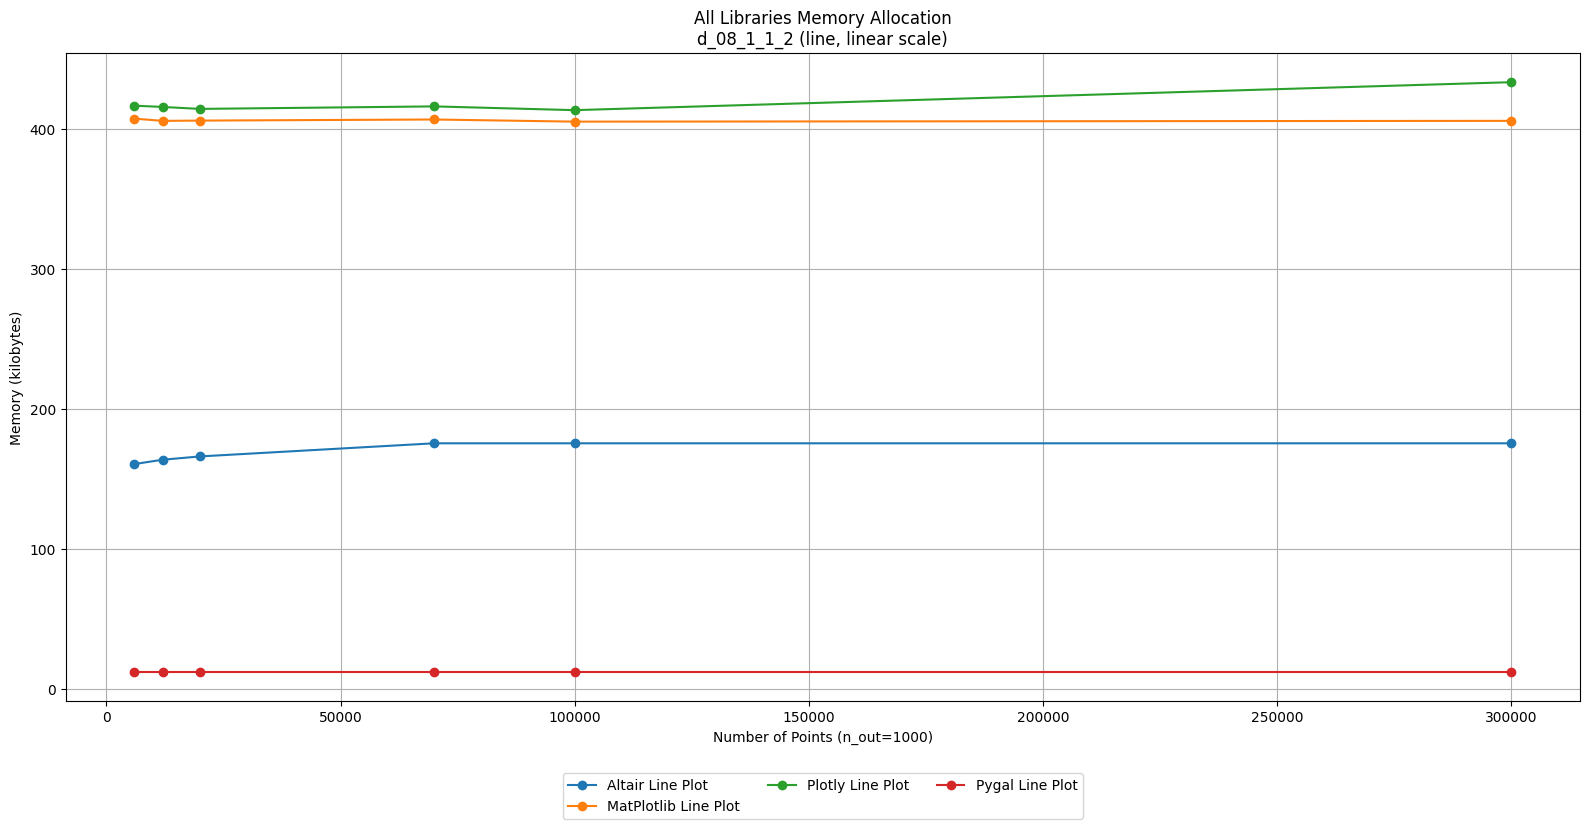
\includegraphics[width=1\textwidth]{anexo/exp/All Libraries Memory Allocation/plots/All Libraries Memory Allocation_d_08_1_1_2_linear_line.png}
        \caption[]{Gráfico de memoria asignada por las diferentes bibliotecas al crear un gráfico para el input \textbf{d\_08\_1\_1\_2}.}
        \label{fig:all_libraries_memory_allocation_plot_line_1}
    \end{figure}
}

\DeclareRobustCommand{\AllLibrariesMemoryAllocationOnePlotBar}{
    %insertar imagen
    \begin{figure}[H]
        \centering
        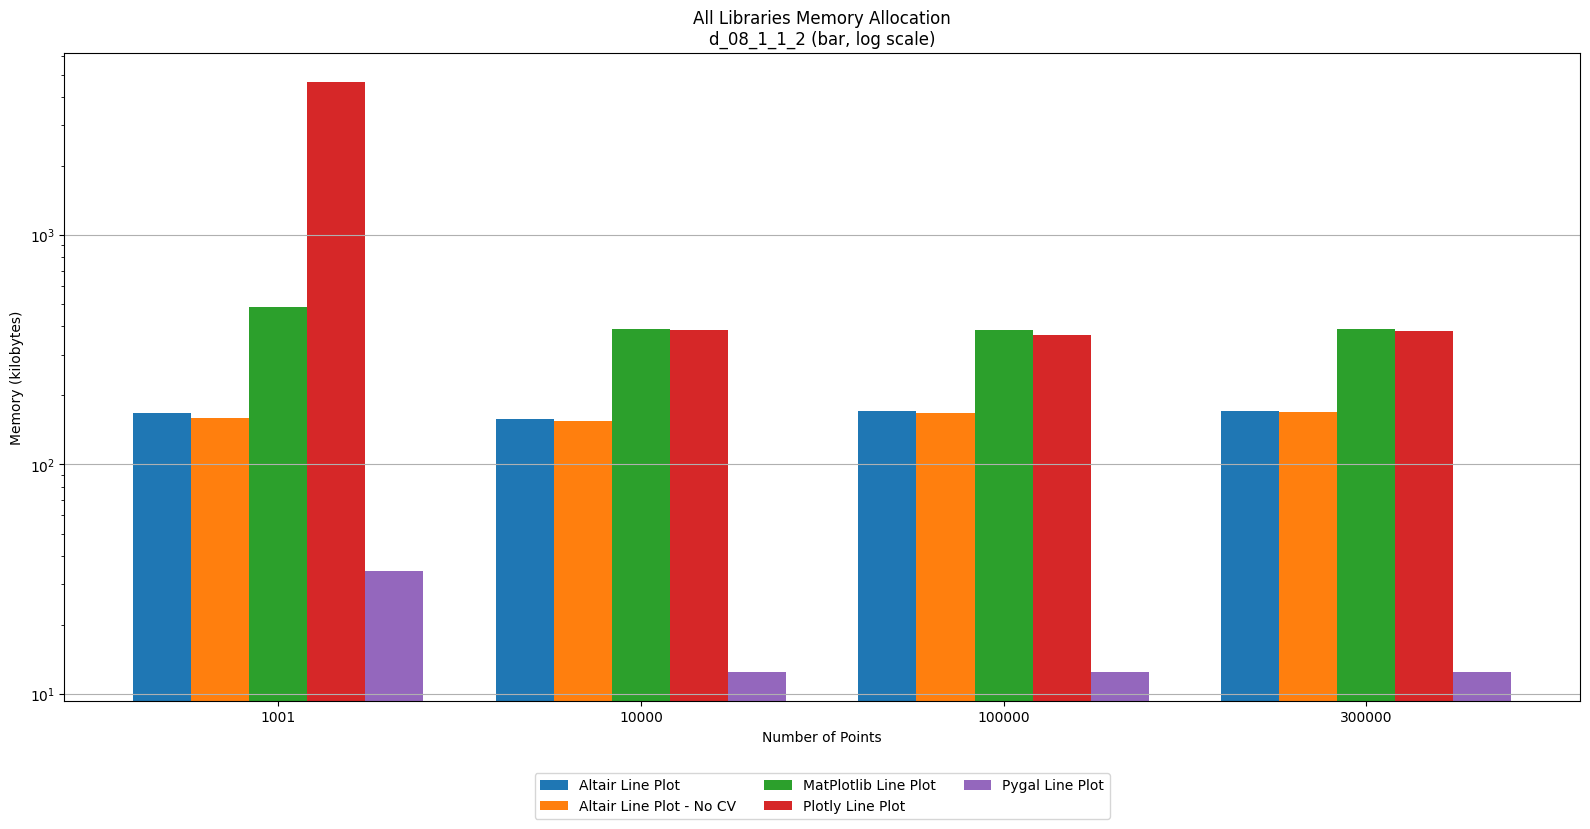
\includegraphics[width=1\textwidth]{anexo/exp/All Libraries Memory Allocation/bar_plots/All Libraries Memory Allocation_d_08_1_1_2_log_bar.png}
        \caption[]{Gráfico de memoria asignada por las diferentes bibliotecas al crear un gráfico para el input \textbf{d\_08\_1\_1\_2}.}
        \label{fig:all_libraries_memory_allocation_plot_bar_1}
    \end{figure}
}

\DeclareRobustCommand{\AllLibrariesMemoryAllocationTwoPlotLine}{
    %insertar imagen
    \begin{figure}[H]
        \centering
        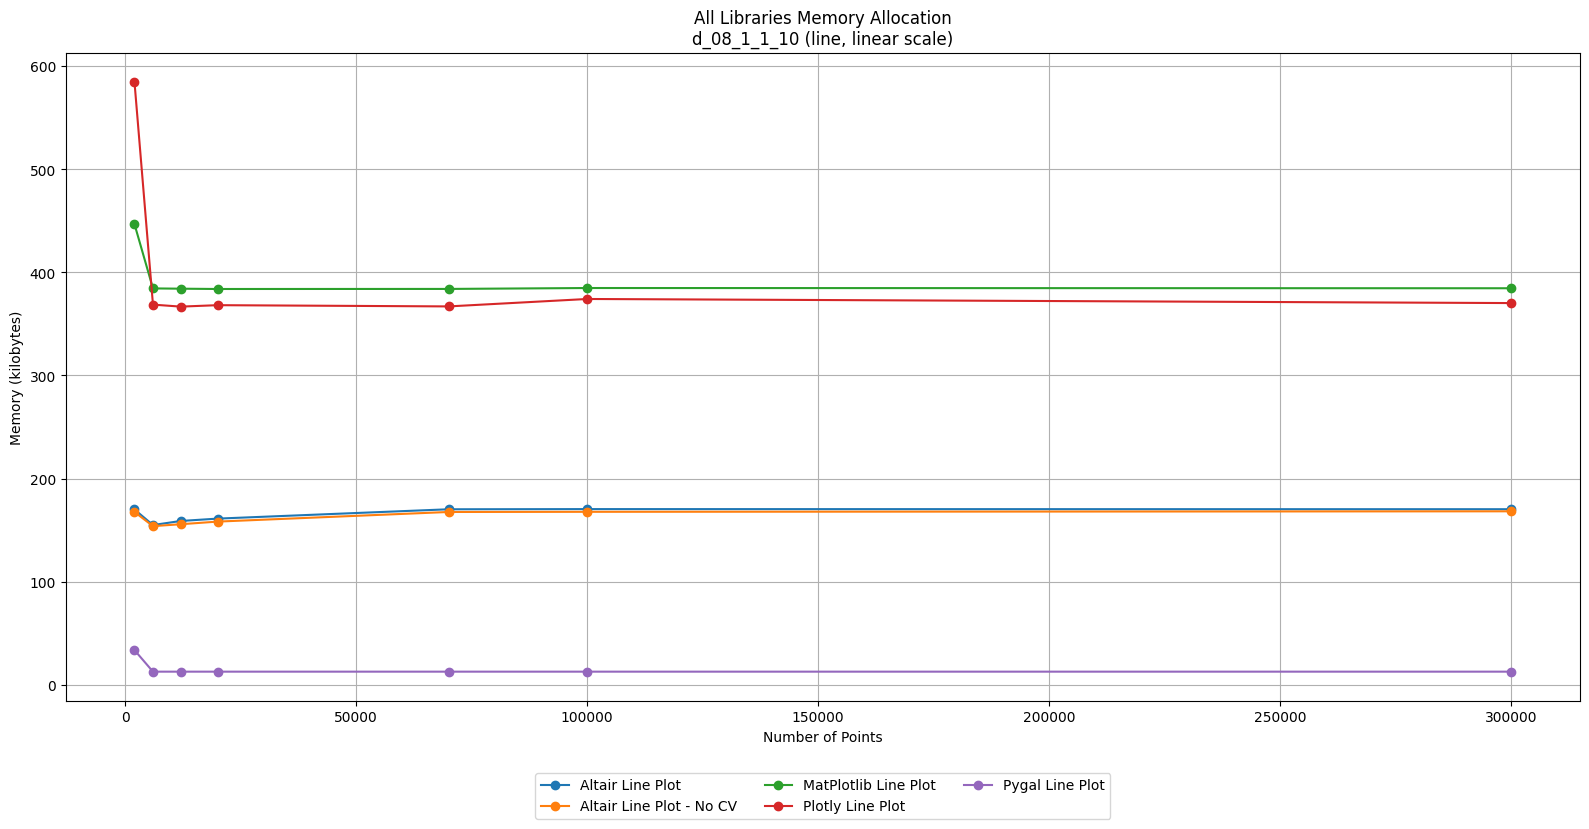
\includegraphics[width=1\textwidth]{anexo/exp/All Libraries Memory Allocation/plots/All Libraries Memory Allocation_d_08_1_1_10_linear_line.png}
        \caption[]{Gráfico de memoria asignada por las diferentes bibliotecas al crear un gráfico para el input \textbf{d\_08\_1\_1\_10}.}
        \label{fig:all_libraries_memory_allocation_plot_line_2}
    \end{figure}
}

\DeclareRobustCommand{\AllLibrariesMemoryAllocationTwoPlotBar}{
    %insertar imagen
    \begin{figure}[H]
        \centering
        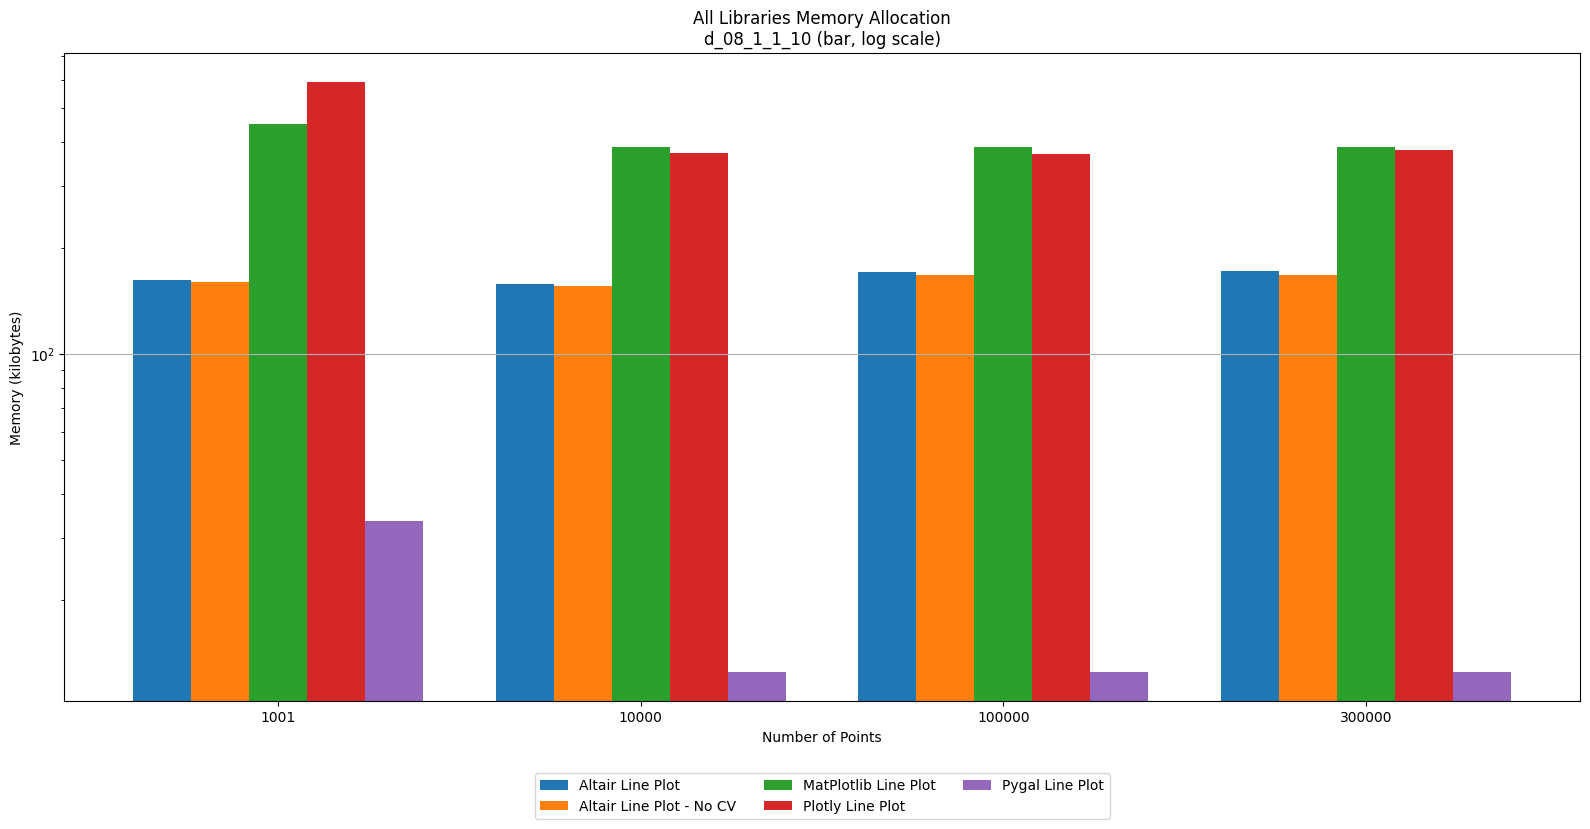
\includegraphics[width=1\textwidth]{anexo/exp/All Libraries Memory Allocation/bar_plots/All Libraries Memory Allocation_d_08_1_1_10_log_bar.png}
        \caption[]{Gráfico de memoria asignada por las diferentes bibliotecas al crear un gráfico para el input \textbf{d\_08\_1\_1\_10}.}
        \label{fig:all_libraries_memory_allocation_plot_bar_2}
    \end{figure}
}

\DeclareRobustCommand{\AllLibrariesMemoryAllocationThreePlotLine}{
    %insertar imagen
    \begin{figure}[H]
        \centering
        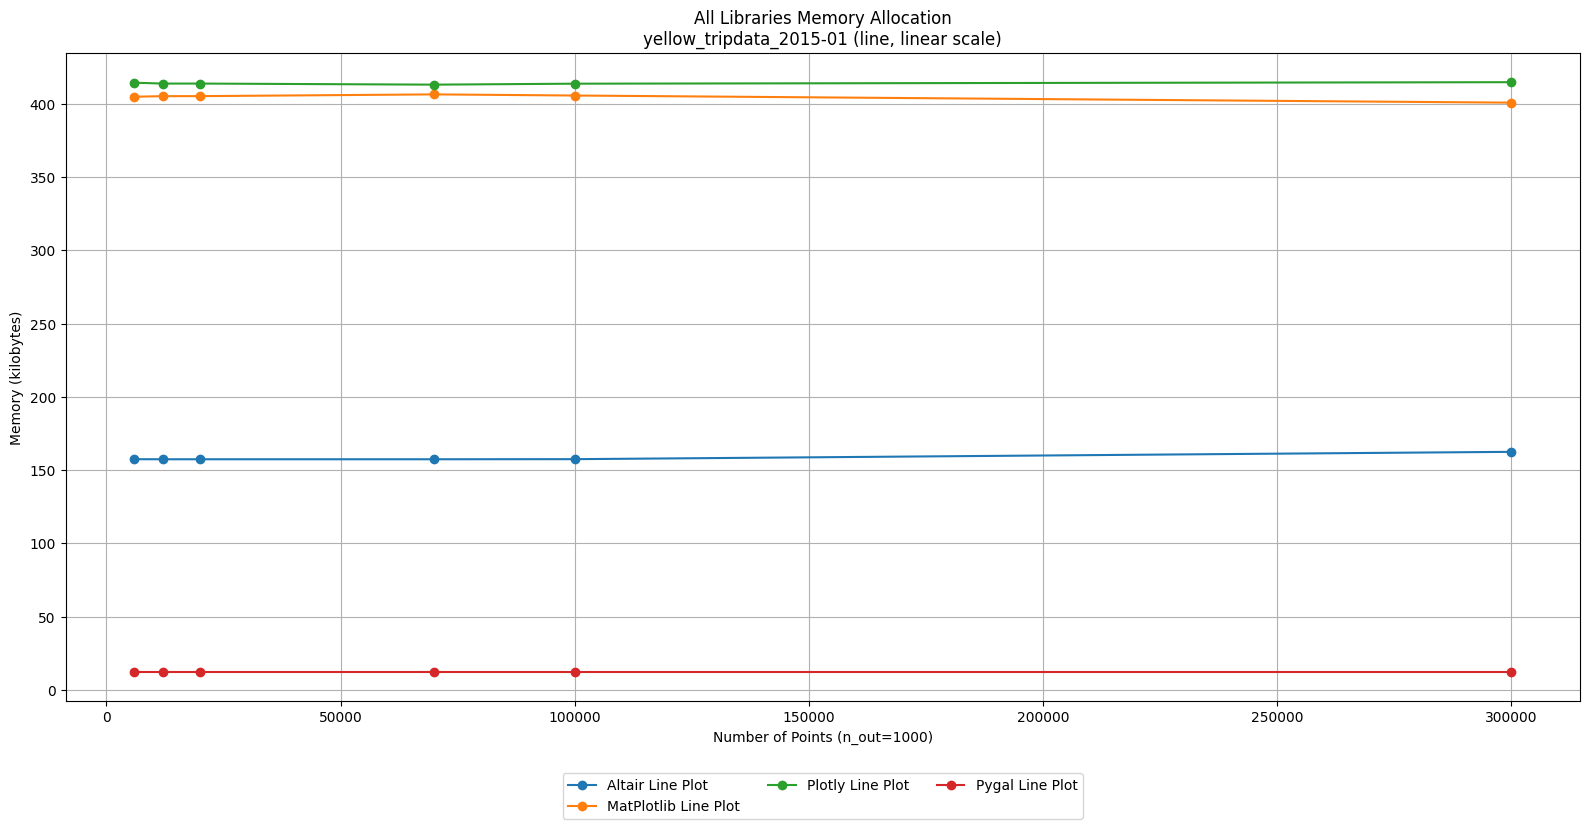
\includegraphics[width=1\textwidth]{anexo/exp/All Libraries Memory Allocation/plots/All Libraries Memory Allocation_yellow_tripdata_2015-01_linear_line.png}
        \caption[]{Gráfico de memoria asignada por las diferentes bibliotecas al crear un gráfico para el input \textbf{yellow\_tripdata\_2015\_01}.}
        \label{fig:all_libraries_memory_allocation_plot_line_3}
    \end{figure}
}

\DeclareRobustCommand{\AllLibrariesMemoryAllocationThreePlotBar}{
    %insertar imagen
    \begin{figure}[H]
        \centering
        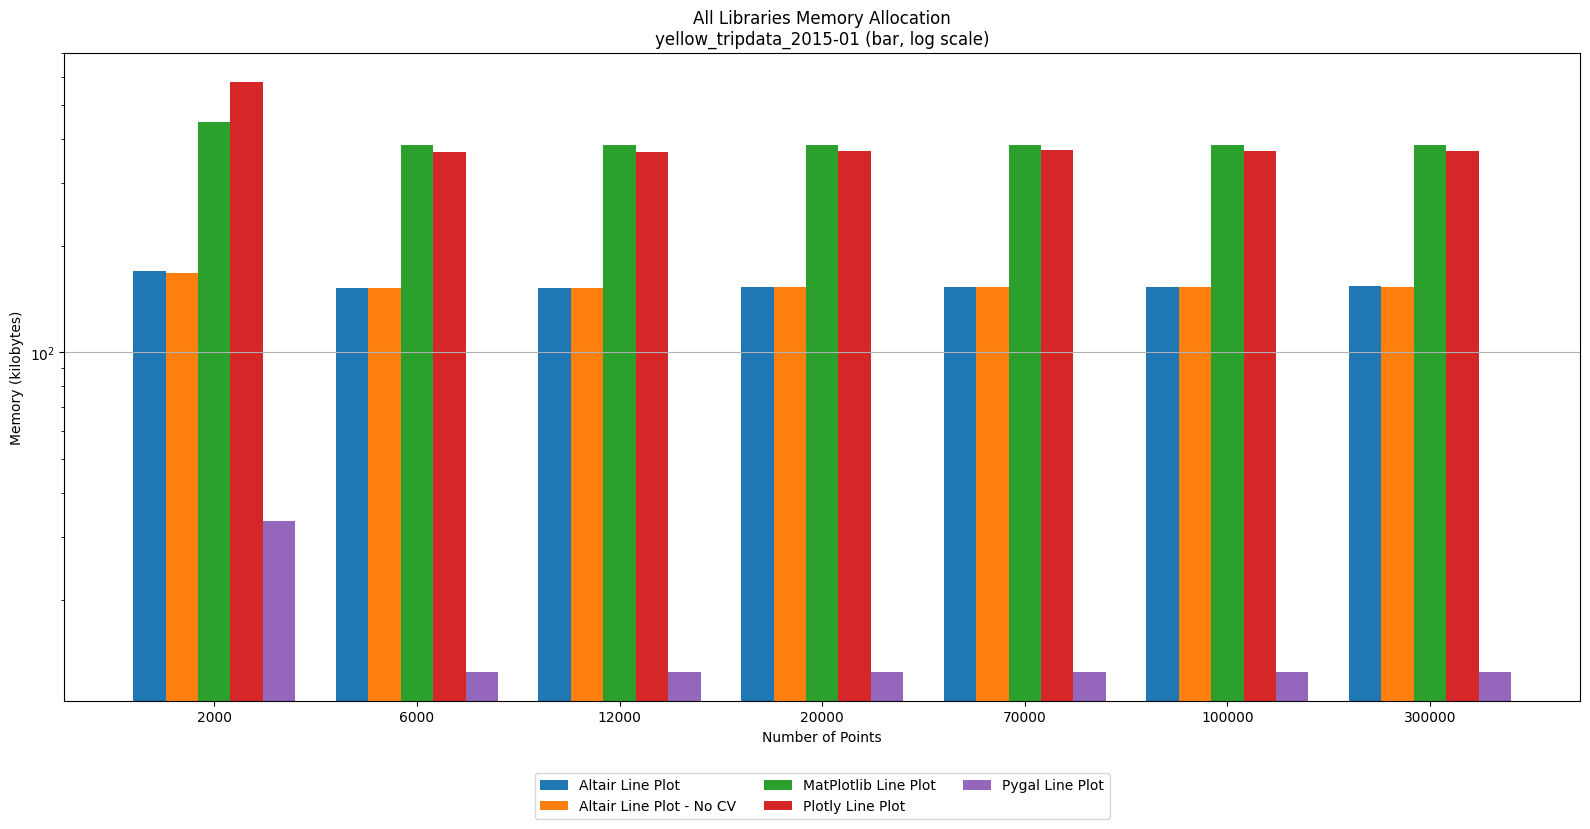
\includegraphics[width=1\textwidth]{anexo/exp/All Libraries Memory Allocation/bar_plots/All Libraries Memory Allocation_yellow_tripdata_2015-01_log_bar.png}
        \caption[]{Gráfico de memoria asignada por las diferentes bibliotecas al crear un gráfico para el input \textbf{yellow\_tripdata\_2015\_01}.}
        \label{fig:all_libraries_memory_allocation_plot_bar_3}
    \end{figure}
}




% All Libraries Time Comparison
\DeclareRobustCommand{\AllLibrariesTimeComparisonOnePlotLine}{
    %insertar imagen
    \begin{figure}[H]
        \centering
        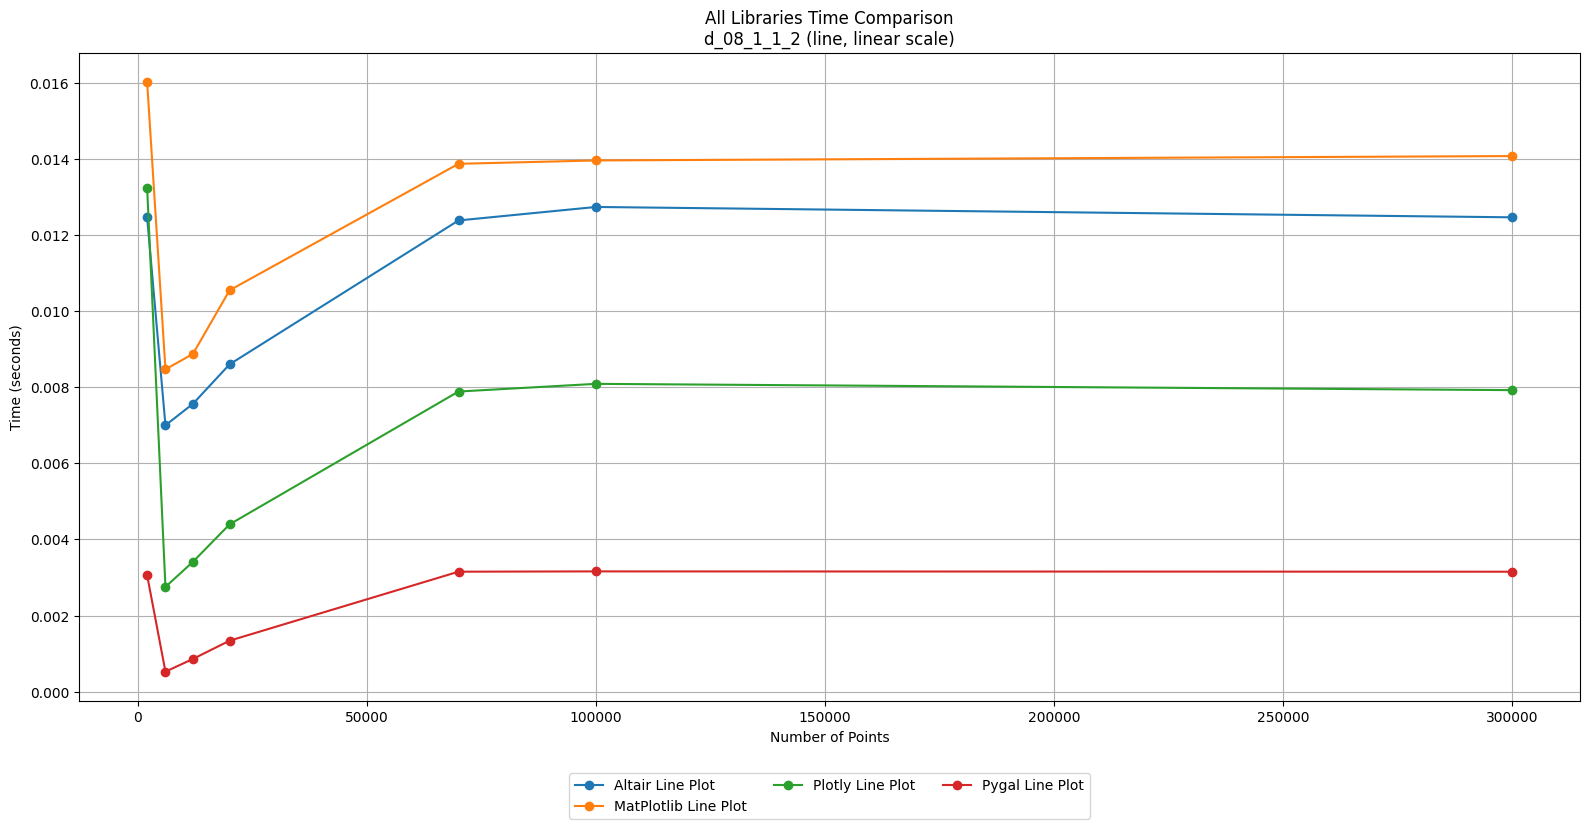
\includegraphics[width=1\textwidth]{anexo/exp/All Libraries Time Comparison/plots/All Libraries Time Comparison_d_08_1_1_2_linear_line.png}
        \caption[]{Gráfico de tiempo de ejecución de las diferentes bibliotecas al crear un gráfico para el input \textbf{d\_08\_1\_1\_2}.}
        \label{fig:all_libraries_time_comparison_plot_line_1}
    \end{figure}
}

\DeclareRobustCommand{\AllLibrariesTimeComparisonOnePlotBar}{
    %insertar imagen
    \begin{figure}[H]
        \centering
        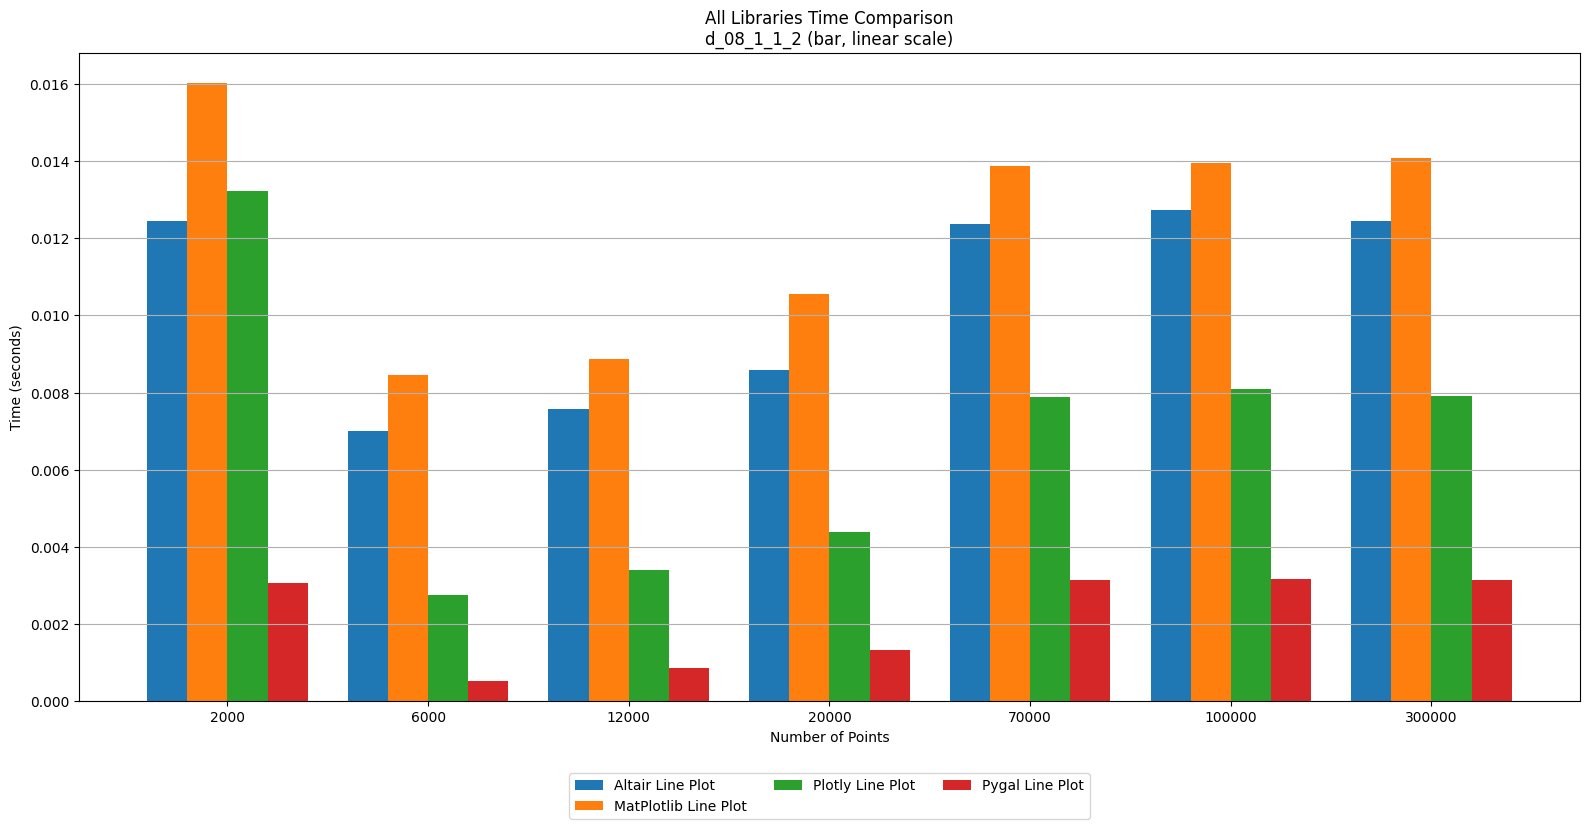
\includegraphics[width=1\textwidth]{anexo/exp/All Libraries Time Comparison/bar_plots/All Libraries Time Comparison_d_08_1_1_2_linear_bar.png}
        \caption[]{Gráfico de tiempo de ejecución de las diferentes bibliotecas al crear un gráfico para el input \textbf{d\_08\_1\_1\_2}.}
        \label{fig:all_libraries_time_comparison_plot_bar_1}
    \end{figure}
}

\DeclareRobustCommand{\AllLibrariesTimeComparisonTwoPlotLine}{
    %insertar imagen
    \begin{figure}[H]
        \centering
        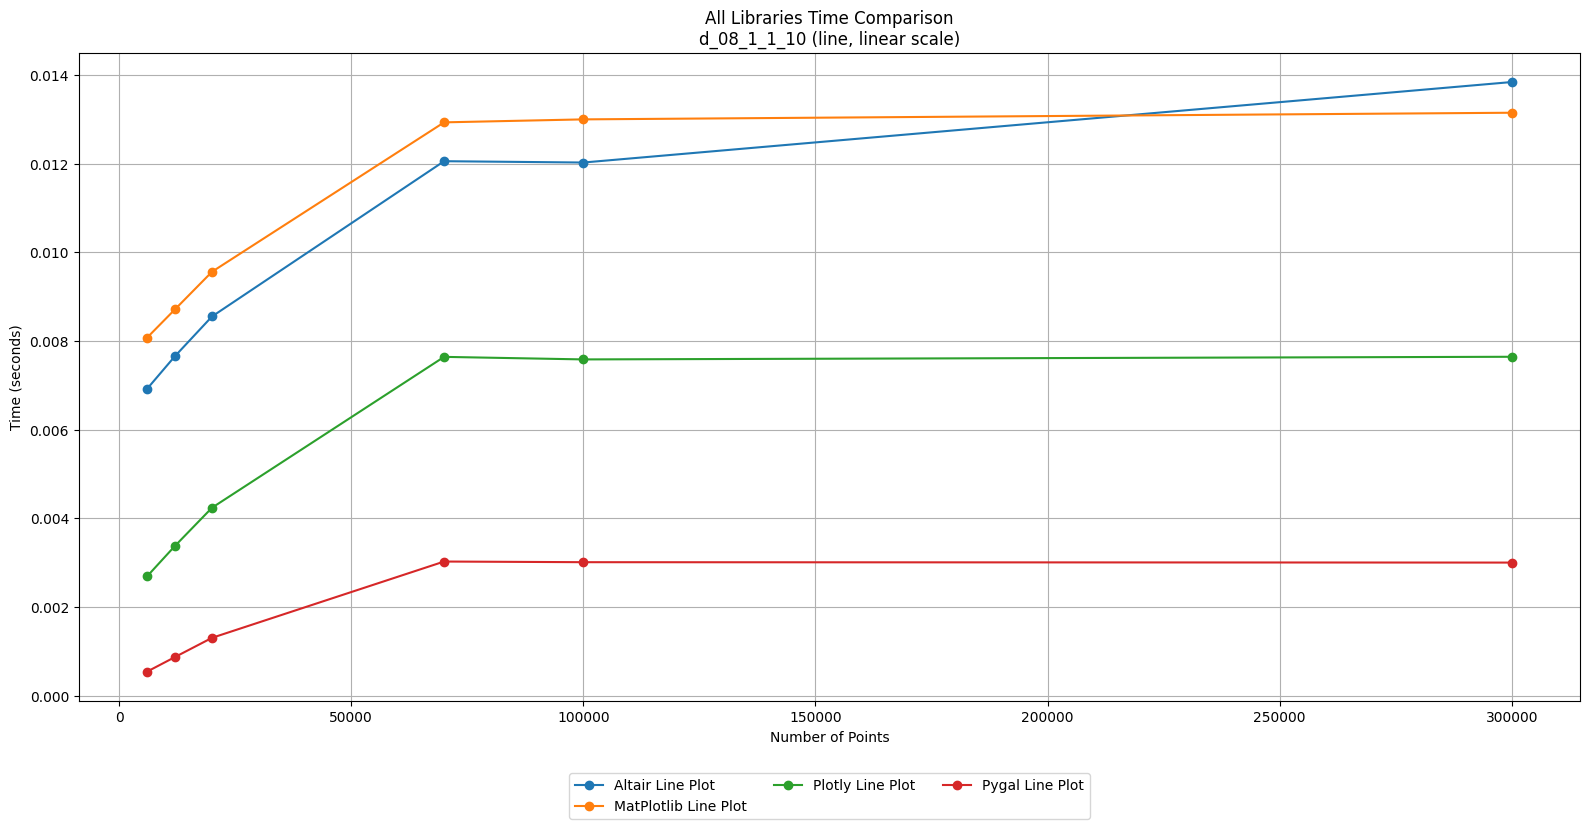
\includegraphics[width=1\textwidth]{anexo/exp/All Libraries Time Comparison/plots/All Libraries Time Comparison_d_08_1_1_10_linear_line.png}
        \caption[]{Gráfico de tiempo de ejecución de las diferentes bibliotecas al crear un gráfico para el input \textbf{d\_08\_1\_1\_10}.}
        \label{fig:all_libraries_time_comparison_plot_line_2}
    \end{figure}
}

\DeclareRobustCommand{\AllLibrariesTimeComparisonTwoPlotBar}{
    %insertar imagen
    \begin{figure}[H]
        \centering
        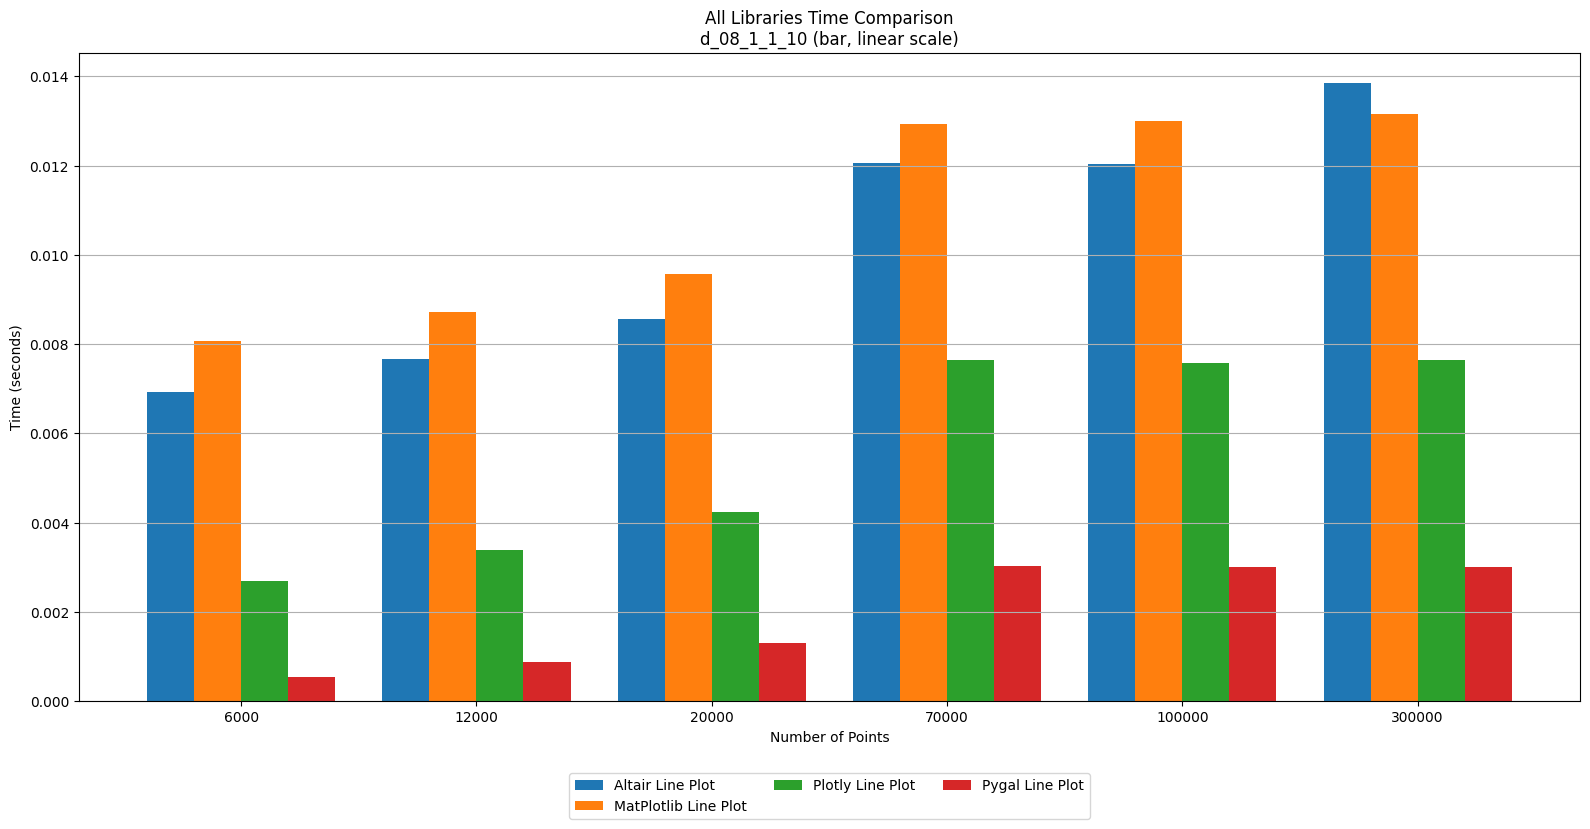
\includegraphics[width=1\textwidth]{anexo/exp/All Libraries Time Comparison/bar_plots/All Libraries Time Comparison_d_08_1_1_10_linear_bar.png}
        \caption[]{Gráfico de tiempo de ejecución de las diferentes bibliotecas al crear un gráfico para el input \textbf{d\_08\_1\_1\_10}.}
        \label{fig:all_libraries_time_comparison_plot_bar_2}
    \end{figure}
}

\DeclareRobustCommand{\AllLibrariesTimeComparisonThreePlotLine}{
    %insertar imagen
    \begin{figure}[H]
        \centering
        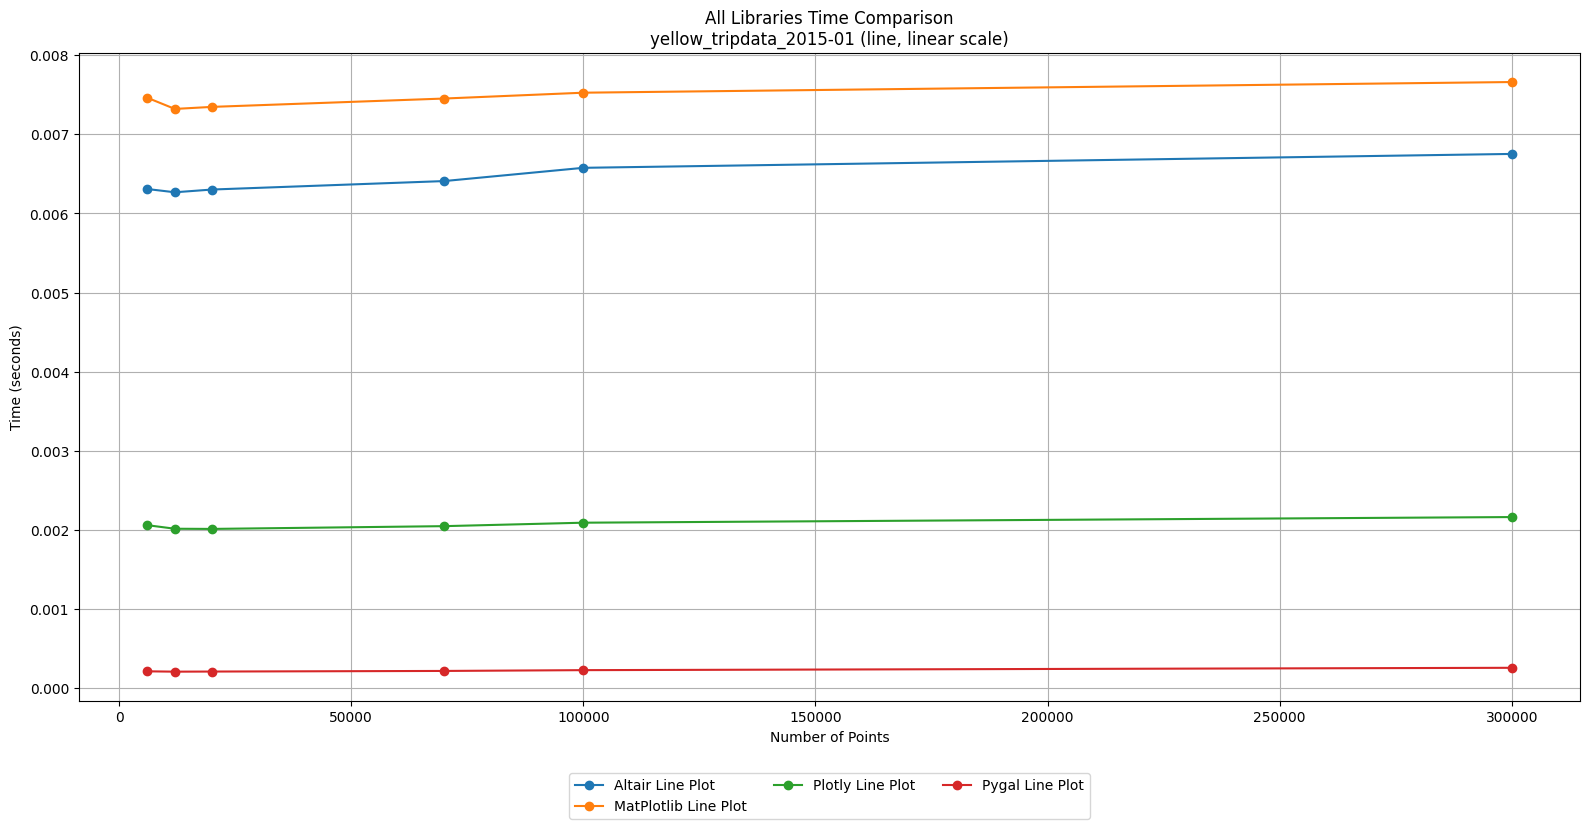
\includegraphics[width=1\textwidth]{anexo/exp/All Libraries Time Comparison/plots/All Libraries Time Comparison_yellow_tripdata_2015-01_linear_line.png}
        \caption[]{Gráfico de tiempo de ejecución de las diferentes bibliotecas al crear un gráfico para el input \textbf{yellow\_tripdata\_2015\_01}.}
        \label{fig:all_libraries_time_comparison_plot_line_3}
    \end{figure}
}

\DeclareRobustCommand{\AllLibrariesTimeComparisonThreePlotBar}{
    %insertar imagen
    \begin{figure}[H]
        \centering
        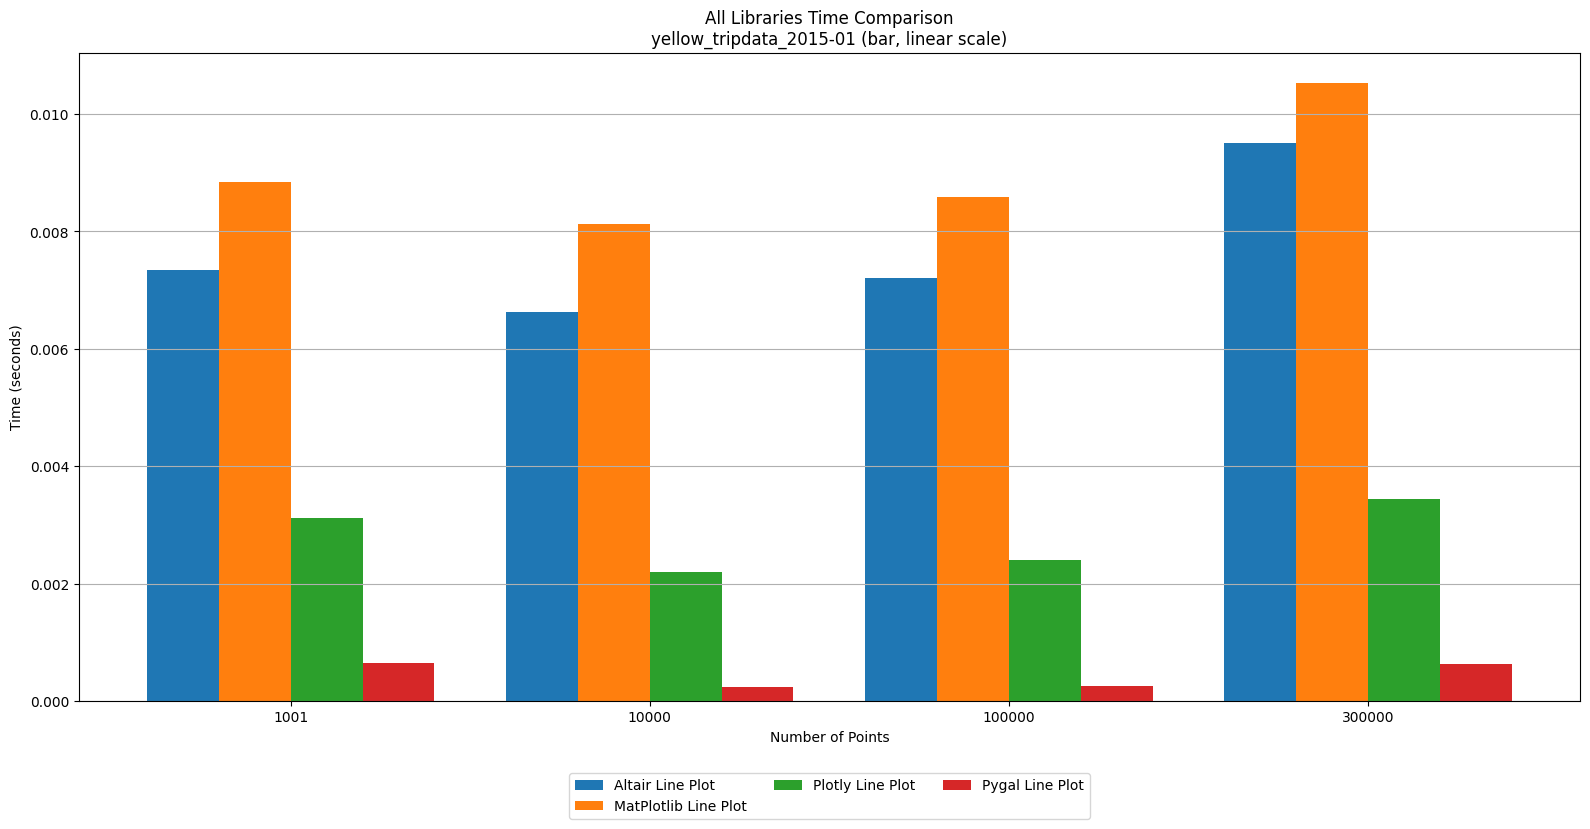
\includegraphics[width=1\textwidth]{anexo/exp/All Libraries Time Comparison/bar_plots/All Libraries Time Comparison_yellow_tripdata_2015-01_linear_bar.png}
        \caption[]{Gráfico de tiempo de ejecución de las diferentes bibliotecas al crear un gráfico para el input \textbf{yellow\_tripdata\_2015\_01}.}
        \label{fig:all_libraries_time_comparison_plot_bar_3}
    \end{figure}
}

Building Time Comparison
\DeclareRobustCommand{\BuildingTimeComparisonOnePlotLine}{
    %insertar imagen
    \begin{figure}[H]
        \centering
        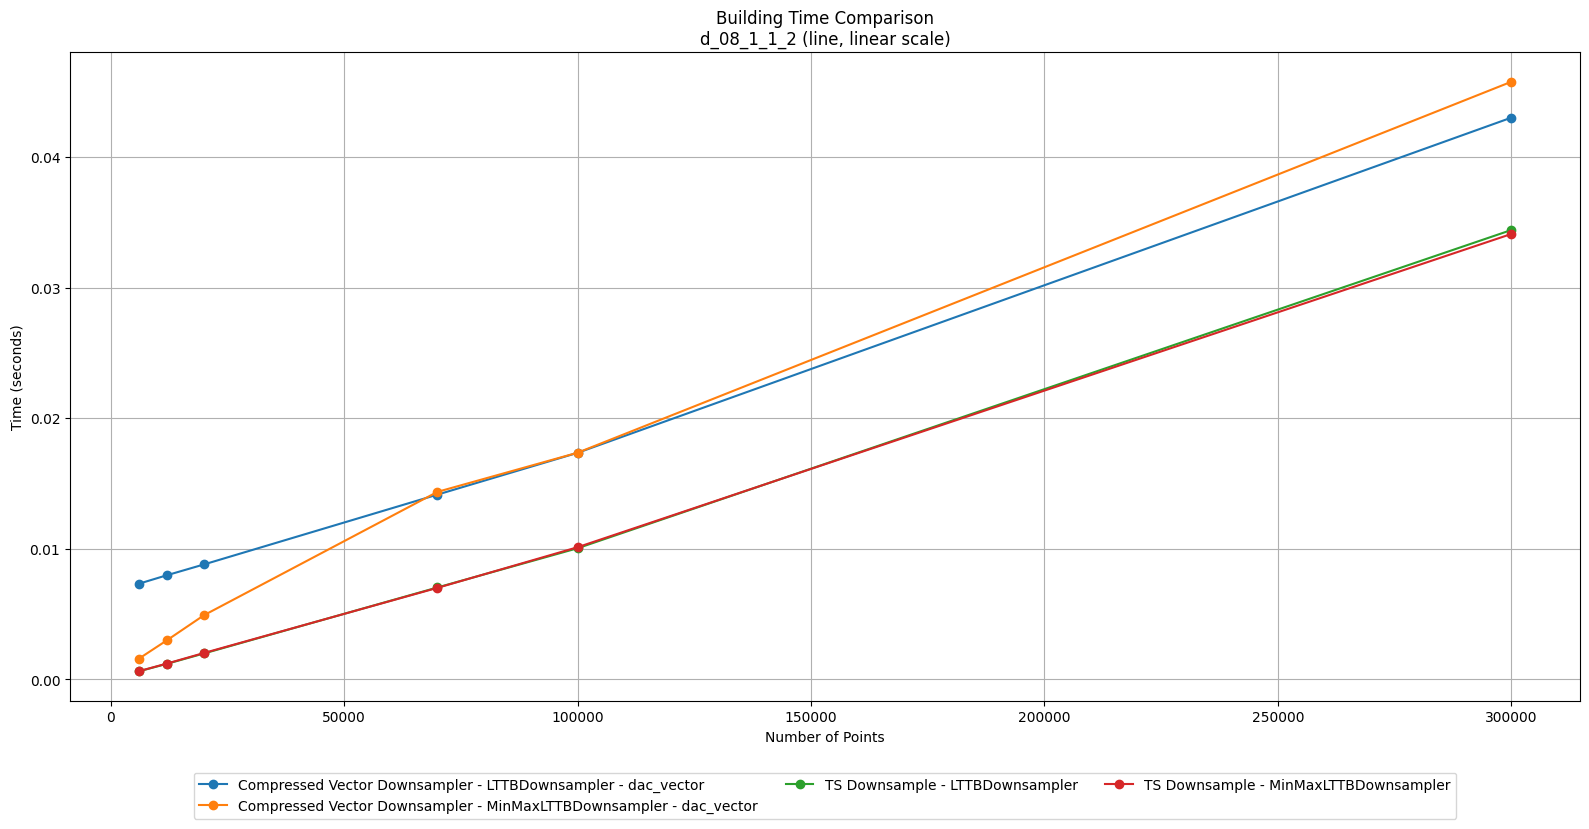
\includegraphics[width=1\textwidth]{anexo/exp/Building Time Comparison/plots/Building Time Comparison_d_08_1_1_2_linear_line.png}
        \caption[]{Gráfico de tiempo de construcción de las diferentes bibliotecas para el input \textbf{d\_08\_1\_1\_2}.}
        \label{fig:building_time_comparison_plot_line_1}
    \end{figure}
}

\DeclareRobustCommand{\BuildingTimeComparisonOnePlotBar}{
    %insertar imagen
    \begin{figure}[H]
        \centering
        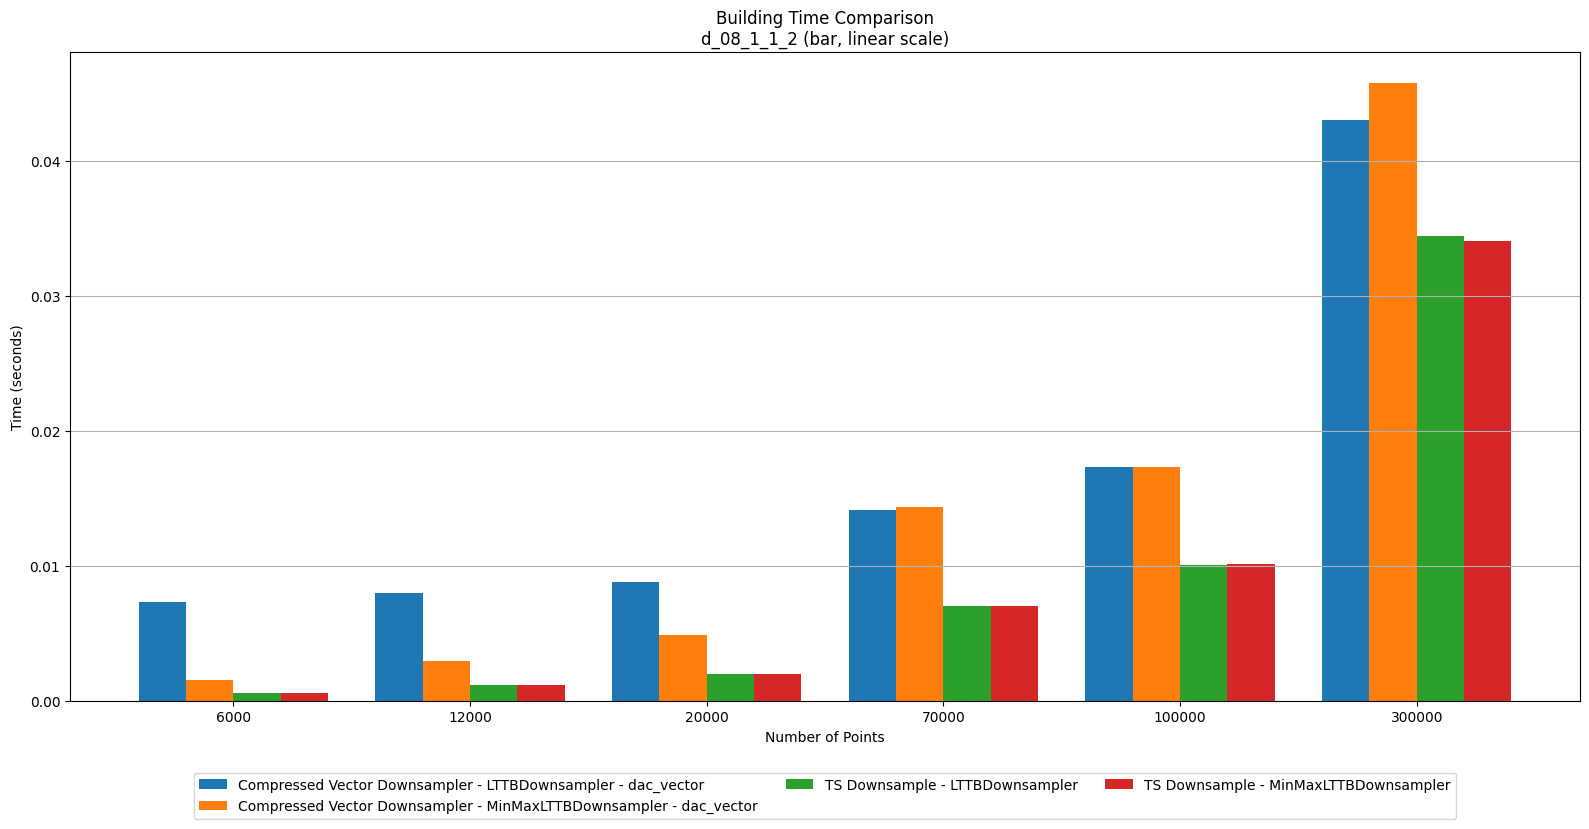
\includegraphics[width=1\textwidth]{anexo/exp/Building Time Comparison/bar_plots/Building Time Comparison_d_08_1_1_2_linear_bar.png}
        \caption[]{Gráfico de tiempo de construcción de las diferentes bibliotecas para el input \textbf{d\_08\_1\_1\_2}.}
        \label{fig:building_time_comparison_plot_bar_1}
    \end{figure}
}

\DeclareRobustCommand{\BuildingTimeComparisonTwoPlotLine}{
    %insertar imagen
    \begin{figure}[H]
        \centering
        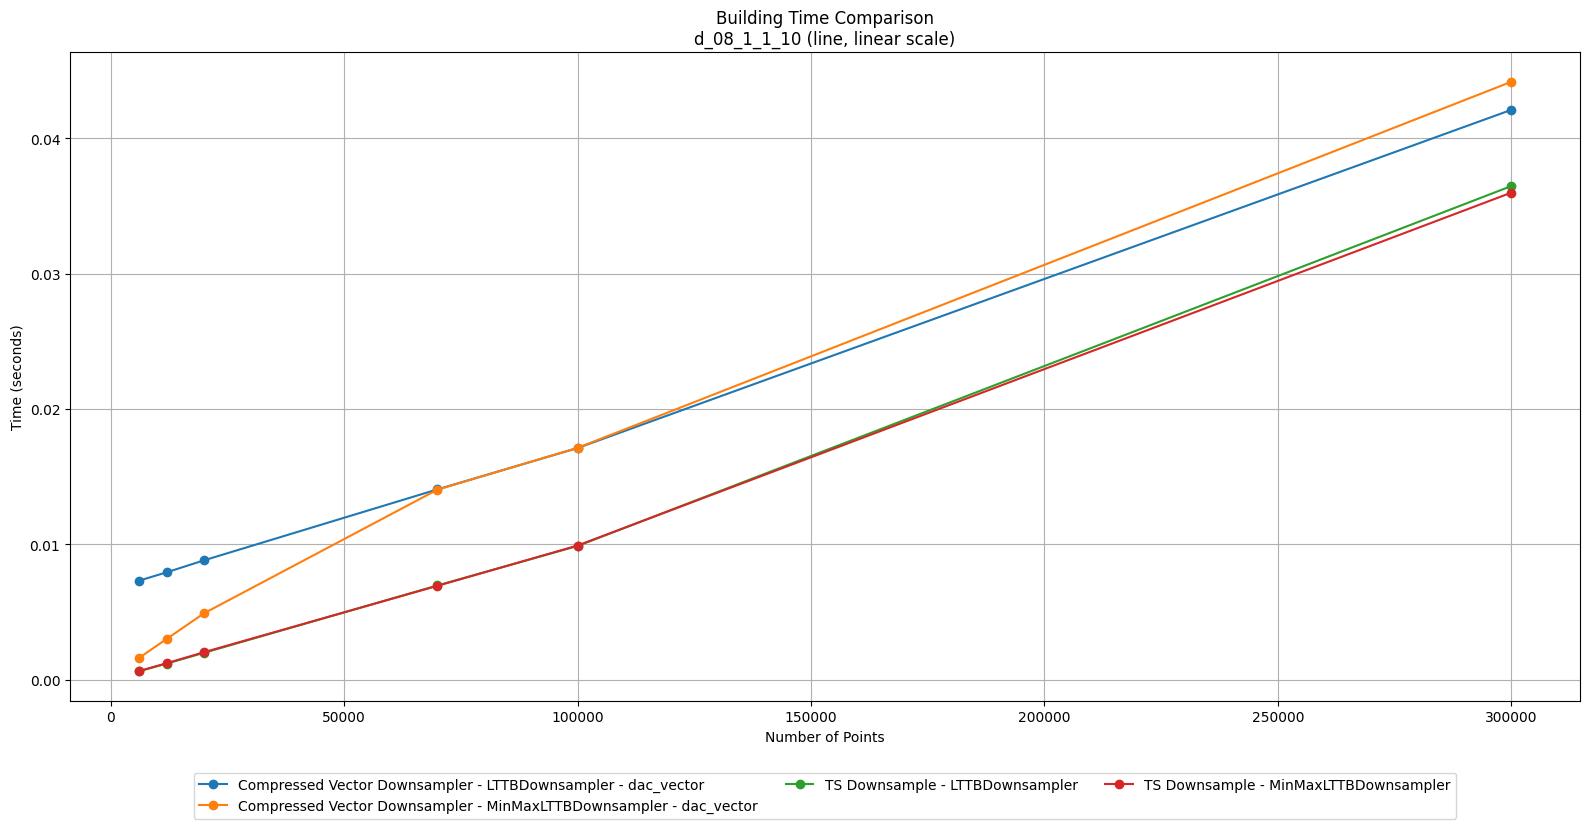
\includegraphics[width=1\textwidth]{anexo/exp/Building Time Comparison/plots/Building Time Comparison_d_08_1_1_10_linear_line.png}
        \caption[]{Gráfico de tiempo de construcción de las diferentes bibliotecas para el input \textbf{d\_08\_1\_1\_10}.}
        \label{fig:building_time_comparison_plot_line_2}
    \end{figure}
}

\DeclareRobustCommand{\BuildingTimeComparisonTwoPlotBar}{
    %insertar imagen
    \begin{figure}[H]
        \centering
        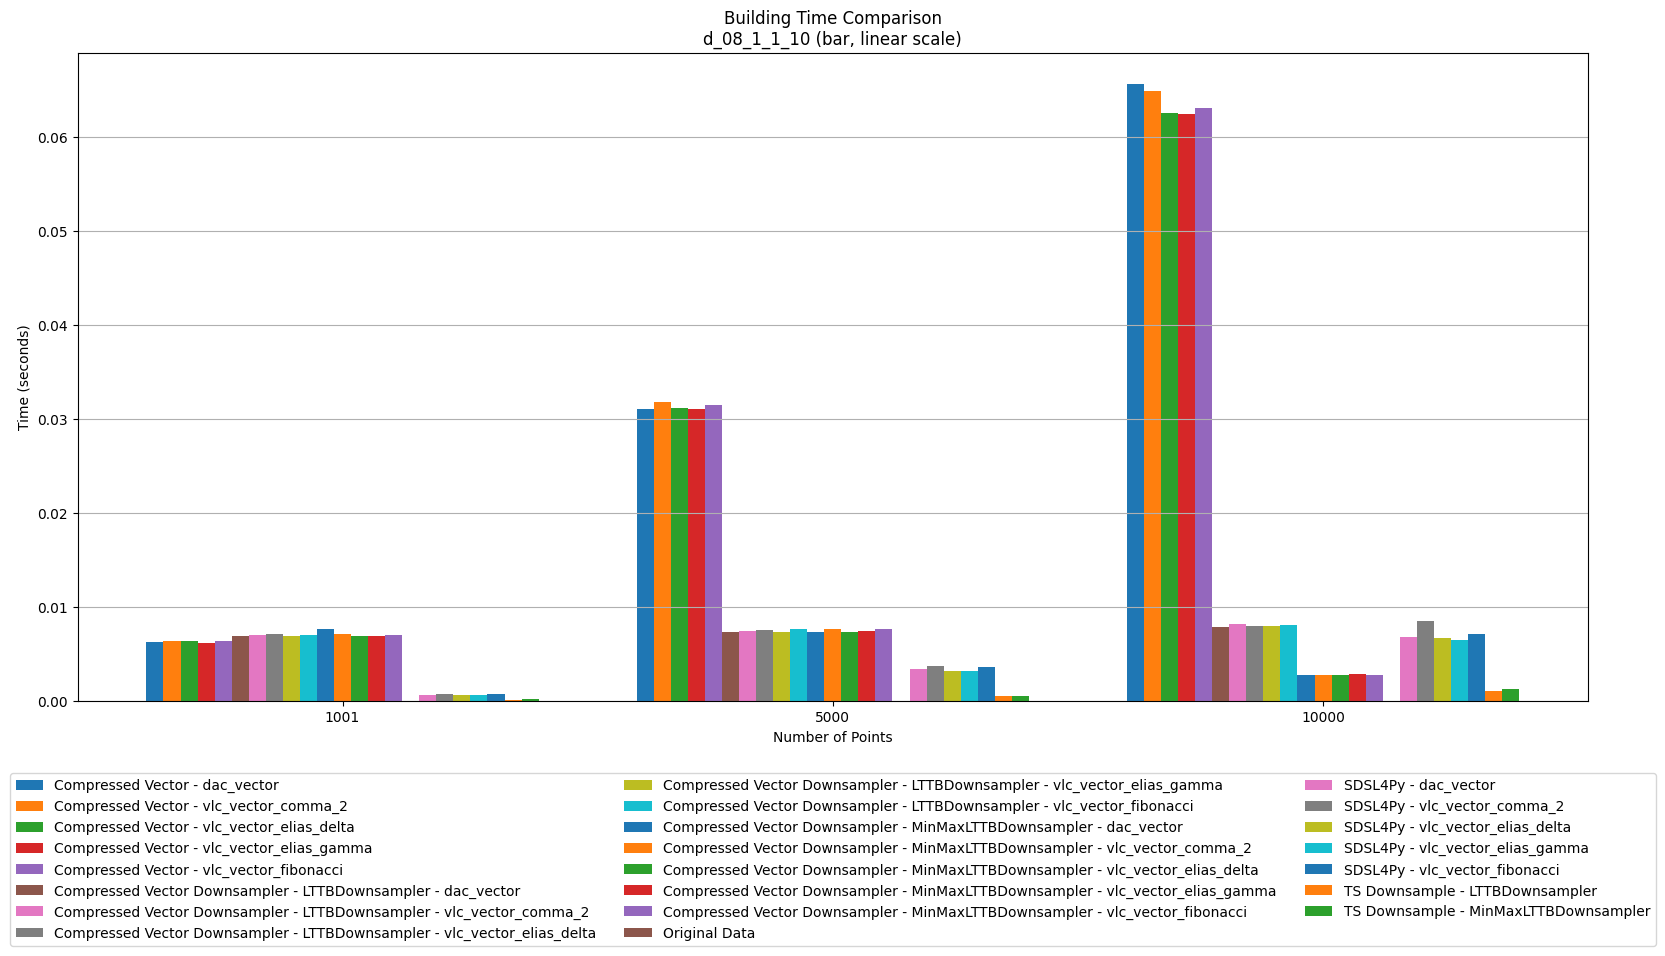
\includegraphics[width=1\textwidth]{anexo/exp/Building Time Comparison/bar_plots/Building Time Comparison_d_08_1_1_10_linear_bar.png}
        \caption[]{Gráfico de tiempo de construcción de las diferentes bibliotecas para el input \textbf{d\_08\_1\_1\_10}.}
        \label{fig:building_time_comparison_plot_bar_2}
    \end{figure}
}

\DeclareRobustCommand{\BuildingTimeComparisonThreePlotLine}{
    %insertar imagen
    \begin{figure}[H]
        \centering
        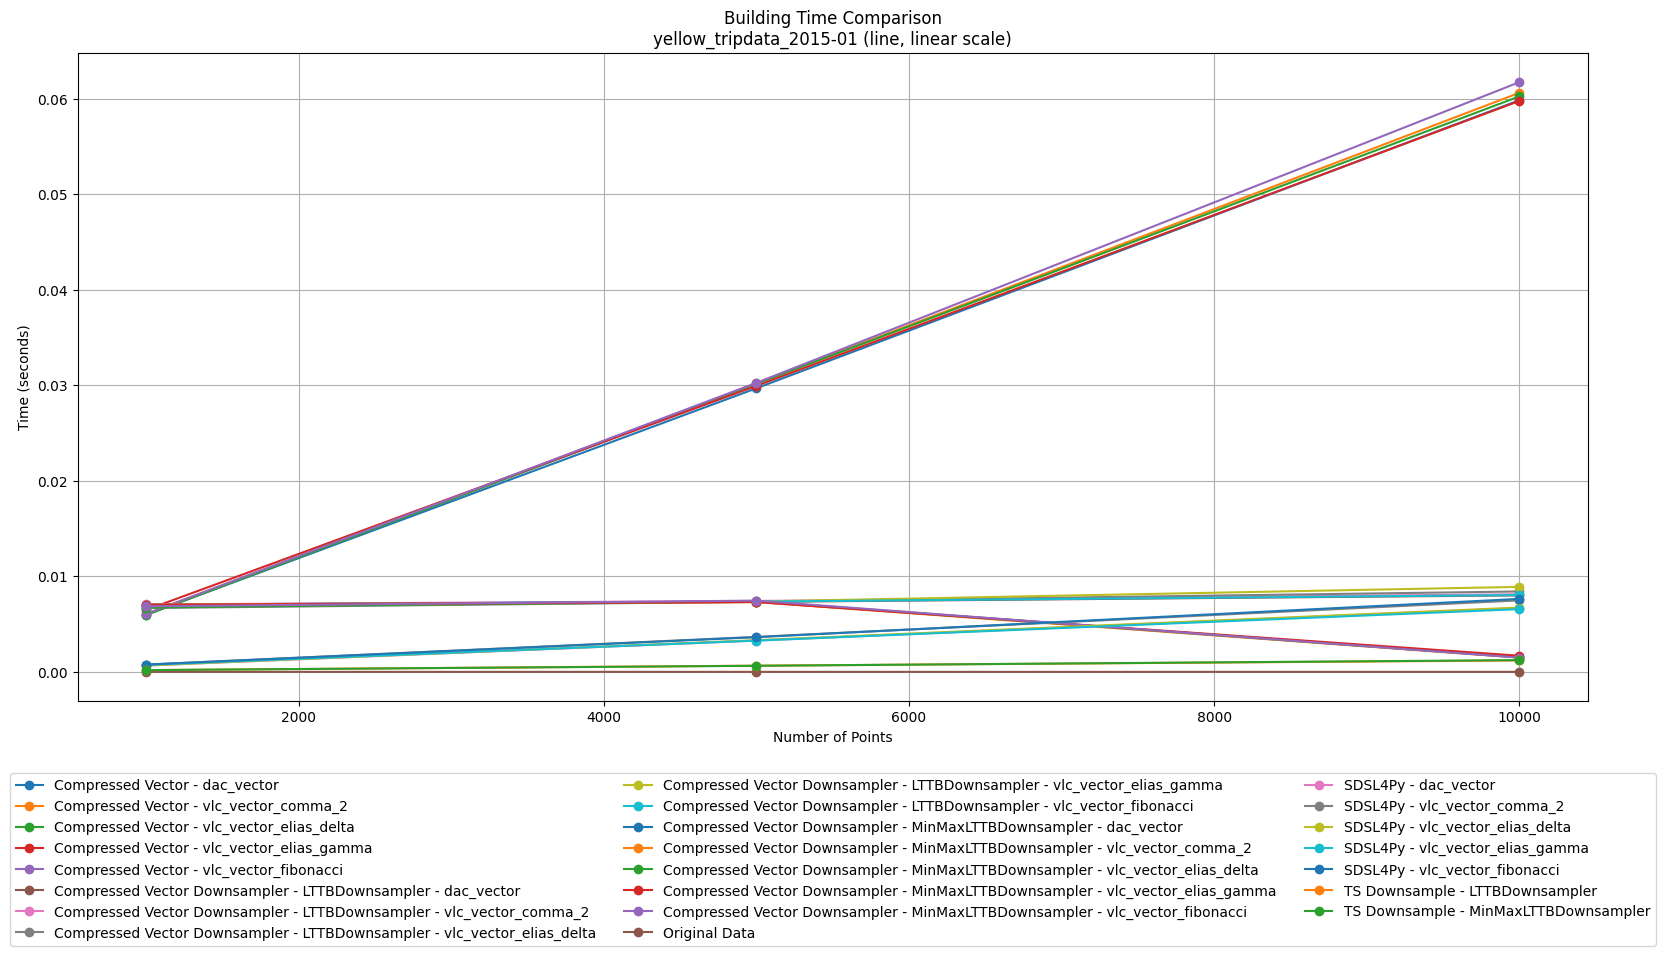
\includegraphics[width=1\textwidth]{anexo/exp/Building Time Comparison/plots/Building Time Comparison_yellow_tripdata_2015-01_linear_line.png}
        \caption[]{Gráfico de tiempo de construcción de las diferentes bibliotecas para el input \textbf{yellow\_tripdata\_2015\_01}.}
        \label{fig:building_time_comparison_plot_line_3}
    \end{figure}
}

\DeclareRobustCommand{\BuildingTimeComparisonThreePlotBar}{
    %insertar imagen
    \begin{figure}[H]
        \centering
        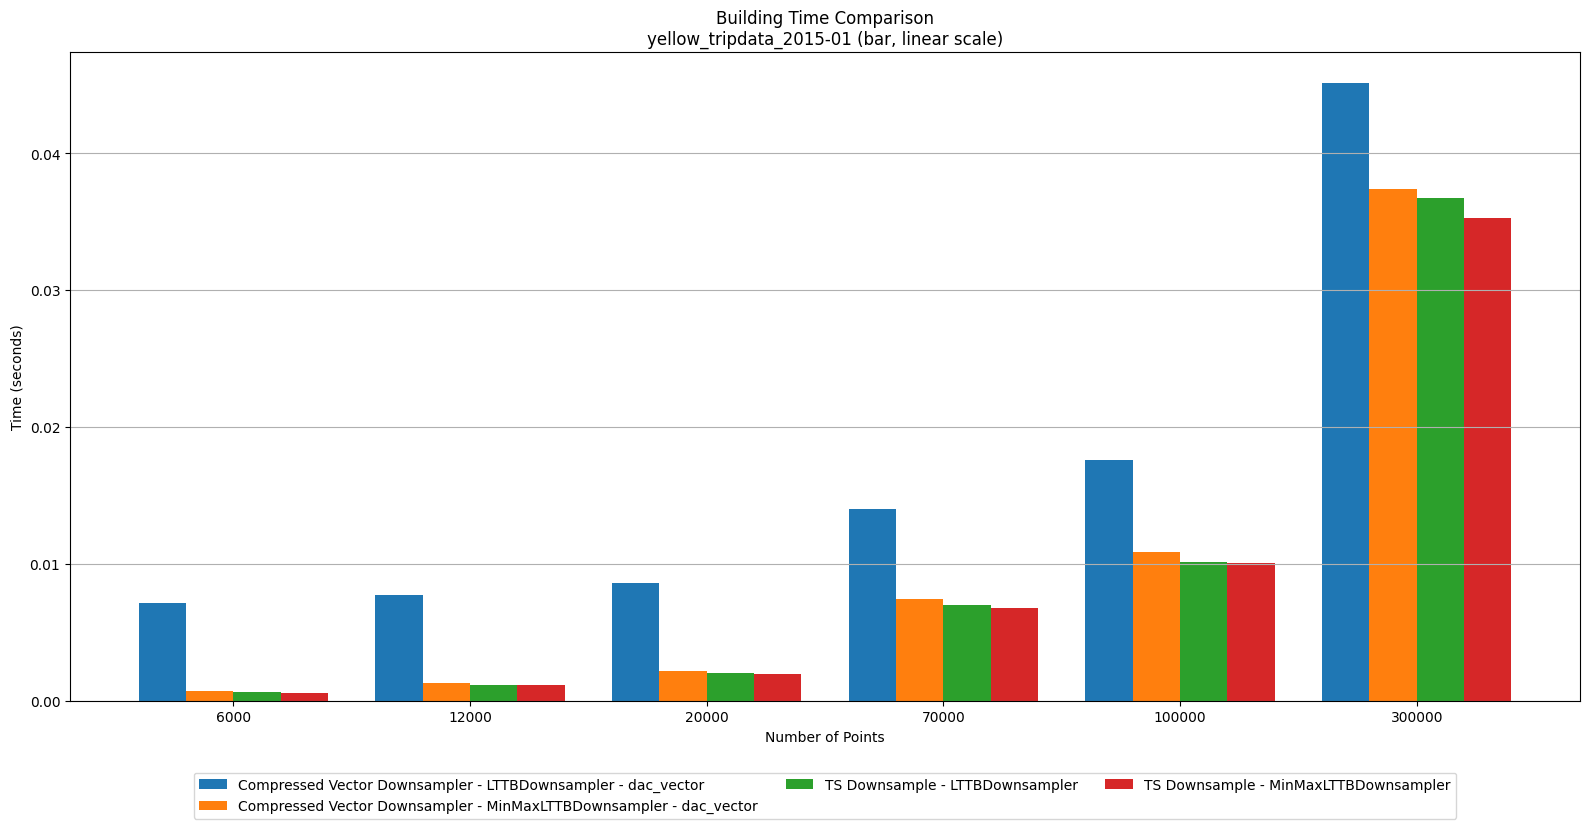
\includegraphics[width=1\textwidth]{anexo/exp/Building Time Comparison/bar_plots/Building Time Comparison_yellow_tripdata_2015-01_linear_bar.png}
        \caption[]{Gráfico de tiempo de construcción de las diferentes bibliotecas para el input \textbf{yellow\_tripdata\_2015\_01}.}
        \label{fig:building_time_comparison_plot_bar_3}
    \end{figure}
}




% Comparison of Space Used
\DeclareRobustCommand{\ComparisonOfSpaceUsedOnePlotLine}{
    %insertar imagen
    \begin{figure}[H]
        \centering
        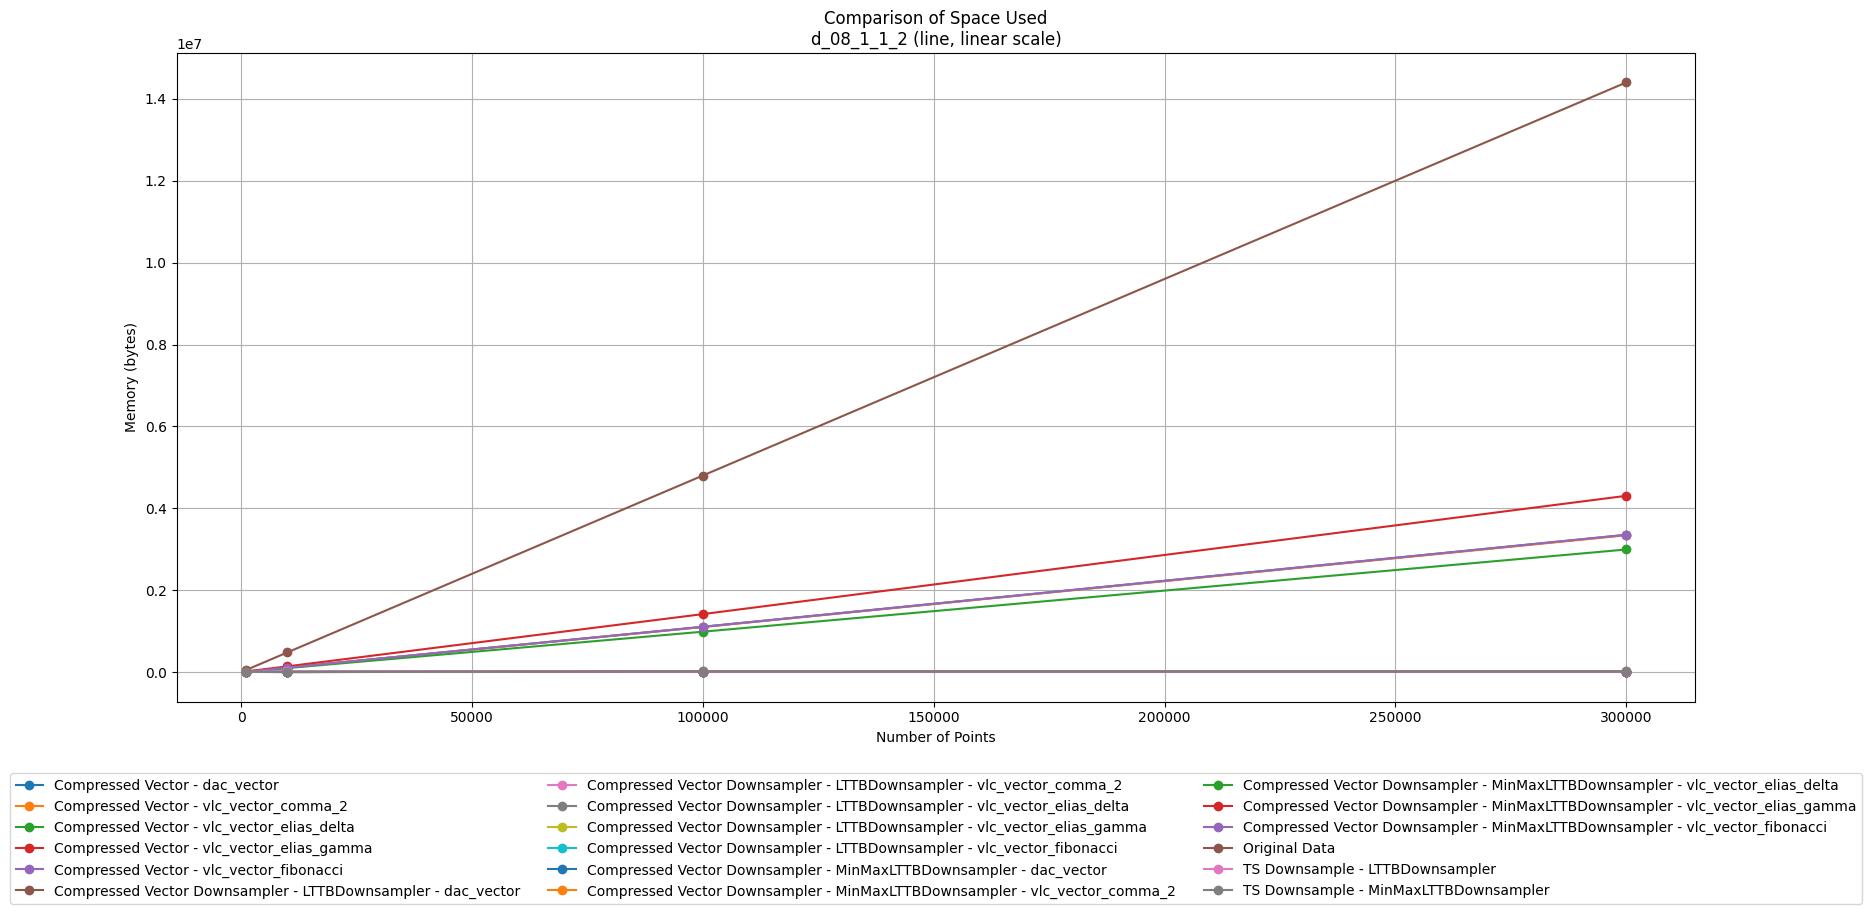
\includegraphics[width=1\textwidth]{anexo/exp/Comparison of Space Used/plots/Comparison of Space Used_d_08_1_1_2_linear_line.png}
        \caption[]{Gráfico de espacio usado por las diferentes bibliotecas para el input \textbf{d\_08\_1\_1\_2}.}
        \label{fig:comparison_of_space_used_plot_line_1}
    \end{figure}
}

\DeclareRobustCommand{\ComparisonOfSpaceUsedOnePlotBar}{
    %insertar imagen
    \begin{figure}[H]
        \centering
        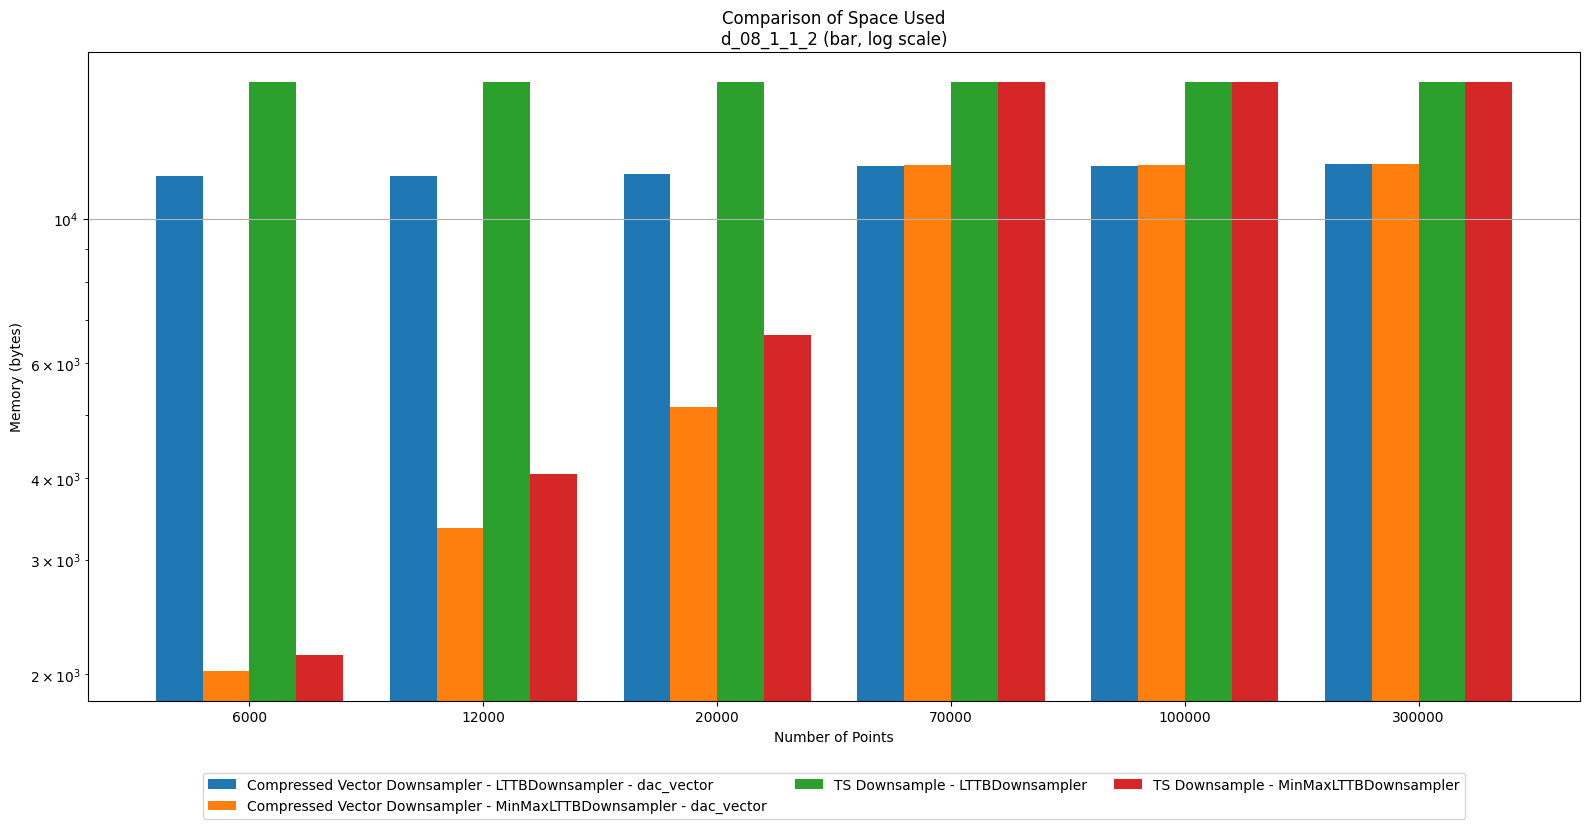
\includegraphics[width=1\textwidth]{anexo/exp/Comparison of Space Used/bar_plots/Comparison of Space Used_d_08_1_1_2_log_bar.png}
        \caption[]{Gráfico de espacio usado por las diferentes bibliotecas para el input \textbf{d\_08\_1\_1\_2}.}
        \label{fig:comparison_of_space_used_plot_bar_1}
    \end{figure}
    \begin{table}[H]
        \centering
        \resizebox{\textwidth}{!}{%
        \begin{tabular}{|l|c|c|c|c|c|c|}
        \hline\multicolumn{1}{|c|}{Option} & \multicolumn{6}{c|}{\textbf{Number of data points}} \\
        \cline{2-7}
         & \textbf{6000} & \textbf{12000} & \textbf{20000} & \textbf{70000} & \textbf{100000} & \textbf{300000} \\
        \hline
        Compressed Vector Downsample - dac\_vector & 1.66e+03 [B] & 2.68e+03 [B] & 4.07e+03 [B] & 9.49e+03 [B] & 9.48e+03 [B] & 9.54e+03 [B] \\
        Compressed Vector Downsample - vlc\_vector\_fibonacci & 1.24e+03 [B] & 2.26e+03 [B] & 3.65e+03 [B] & 8.89e+03 [B] & 8.88e+03 [B] & 9.04e+03 [B] \\
        Original Data & 1.06e+05 [B] & 2.16e+05 [B] & 3.46e+05 [B] & 1.12e+06 [B] & 1.60e+06 [B] & 5.20e+06 [B] \\
        TS Downsample & 2.14e+03 [B] & 4.06e+03 [B] & 6.62e+03 [B] & 1.62e+04 [B] & 1.62e+04 [B] & 1.62e+04 [B] \\
        \hline
        \end{tabular}
        }
        \label{tab:comparison of space used-d-08-1-1-2}
    \end{table}
    \begin{table}[H]
        \centering
        \caption{Comparison of Space Used\_d\_08\_1\_1\_2 – Tasa de compactación CVD vs TS vs Datos Originales}
        \label{tab:Comparison of Space Used\_d\_08\_1\_1\_2_cvd_compactacion}
        \begin{tabular}{rlrr}
        \toprule
        n\_size & Variante & Comp. vs TS (\%) & Comp. vs Original (\%) \\
        \midrule
        6000 & CVD - dac\_vector & 22.48 & 98.43 \\
        6000 & CVD - vlc\_vector\_fibonacci & 42.26 & 98.83 \\
        12000 & CVD - dac\_vector & 34.10 & 98.76 \\
        12000 & CVD - vlc\_vector\_fibonacci & 44.34 & 98.95 \\
        20000 & CVD - dac\_vector & 38.56 & 98.82 \\
        20000 & CVD - vlc\_vector\_fibonacci & 44.96 & 98.95 \\
        70000 & CVD - dac\_vector & 41.53 & 99.16 \\
        70000 & CVD - vlc\_vector\_fibonacci & 45.18 & 99.21 \\
        100000 & CVD - dac\_vector & 41.58 & 99.41 \\
        100000 & CVD - vlc\_vector\_fibonacci & 45.28 & 99.45 \\
        300000 & CVD - dac\_vector & 41.19 & 99.82 \\
        300000 & CVD - vlc\_vector\_fibonacci & 44.29 & 99.83 \\
        \bottomrule
        \end{tabular}
        
    \end{table}
}

\DeclareRobustCommand{\ComparisonOfSpaceUsedTwoPlotLine}{
    %insertar imagen
    \begin{figure}[H]
        \centering
        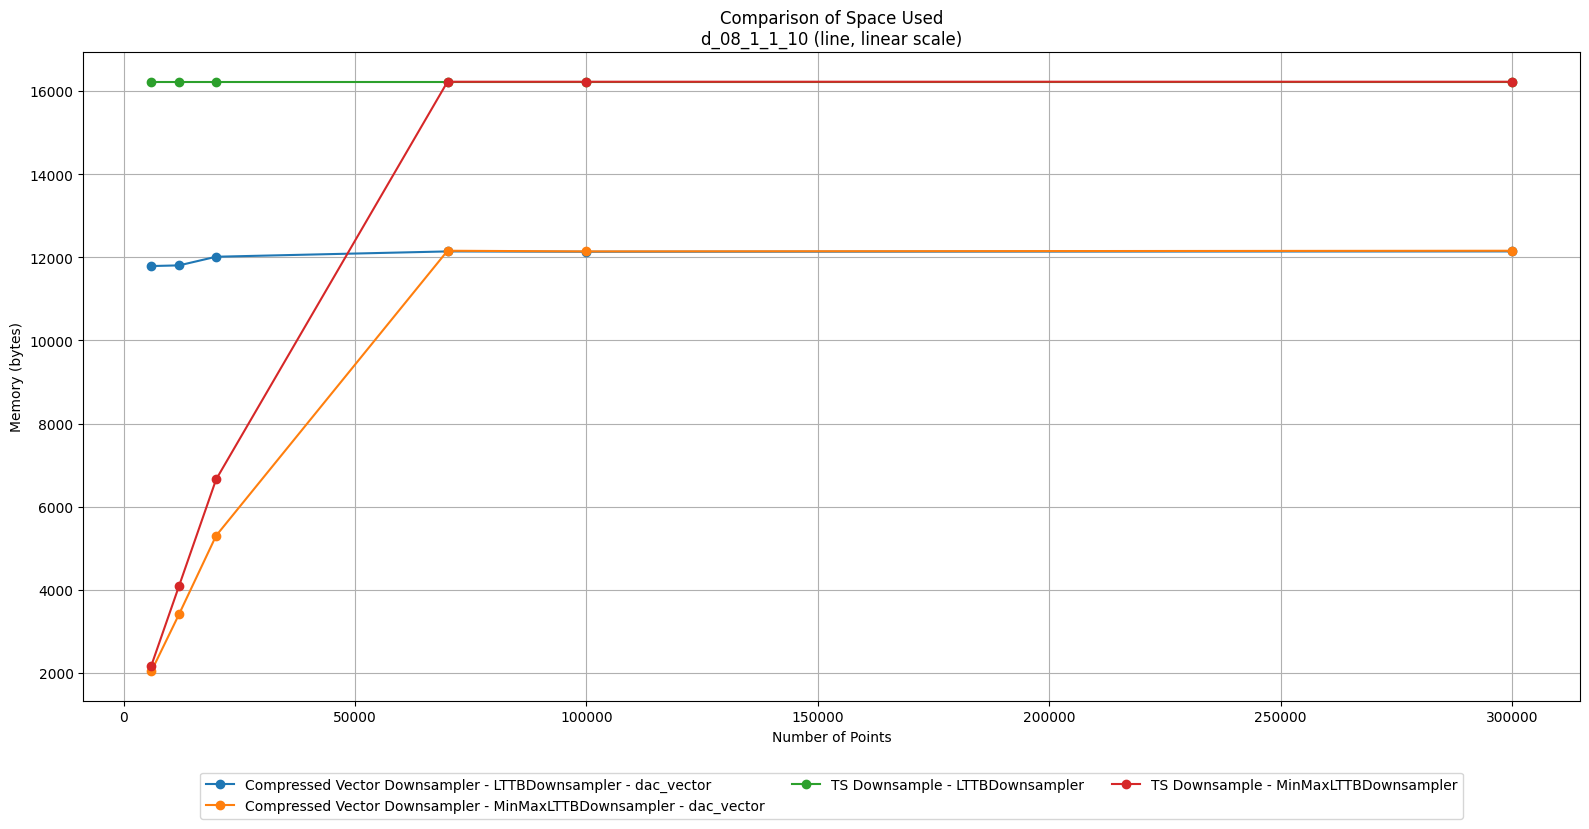
\includegraphics[width=1\textwidth]{anexo/exp/Comparison of Space Used/plots/Comparison of Space Used_d_08_1_1_10_linear_line.png}
        \caption[]{Gráfico de espacio usado por las diferentes bibliotecas para el input \textbf{d\_08\_1\_1\_10}.}
        \label{fig:comparison_of_space_used_plot_line_2}
    \end{figure}
}

\DeclareRobustCommand{\ComparisonOfSpaceUsedTwoPlotBar}{
    %insertar imagen
    \begin{figure}[H]
        \centering
        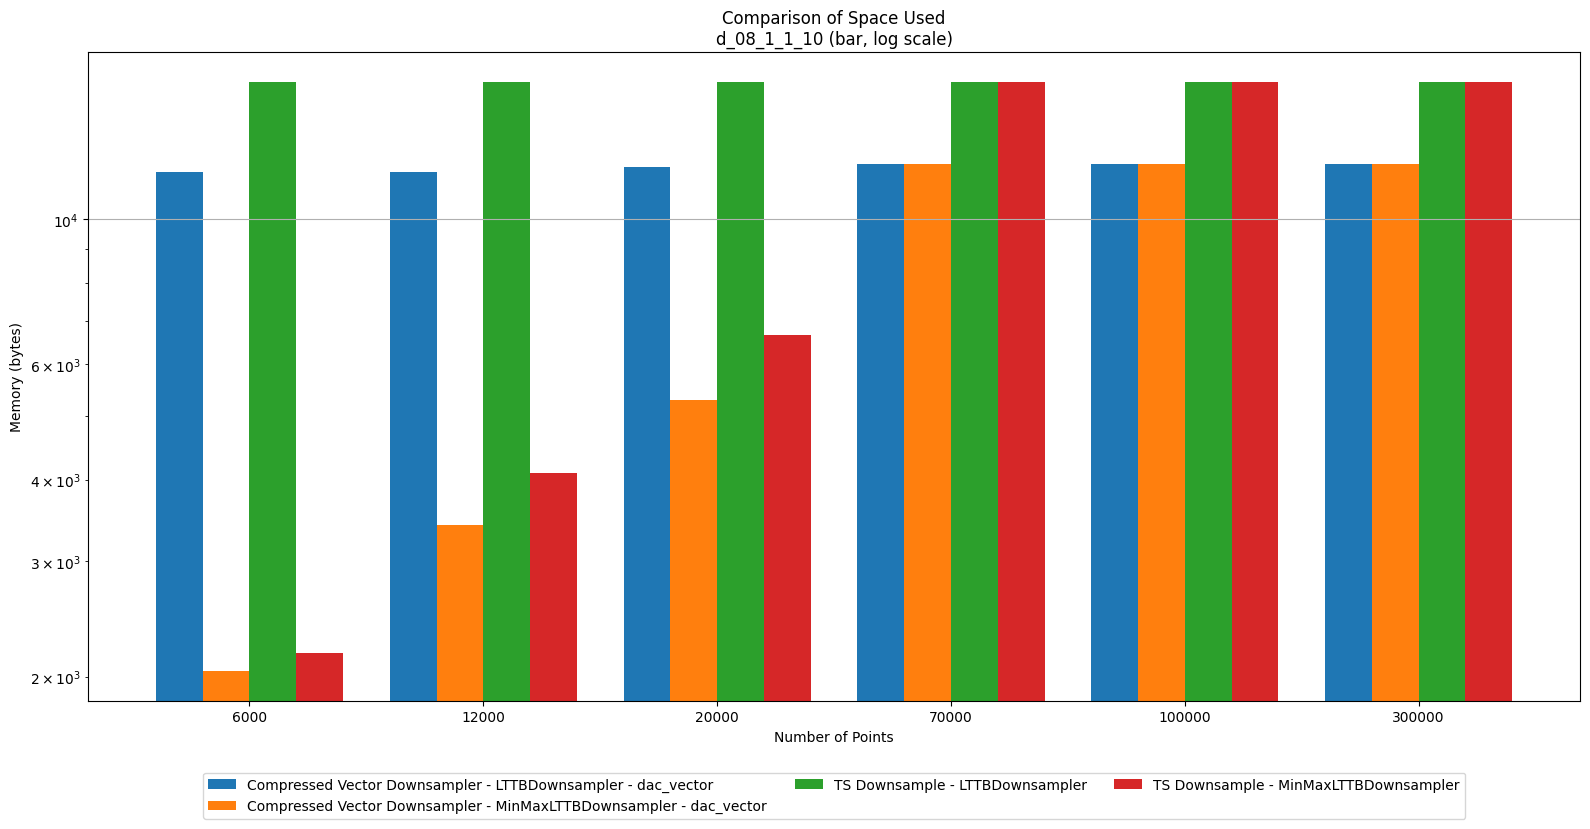
\includegraphics[width=1\textwidth]{anexo/exp/Comparison of Space Used/bar_plots/Comparison of Space Used_d_08_1_1_10_log_bar.png}
        \caption[]{Gráfico de espacio usado por las diferentes bibliotecas para el input \textbf{d\_08\_1\_1\_10}.}
        \label{fig:comparison_of_space_used_plot_bar_2}
    \end{figure}

    \begin{table}[H]
        \centering
        \resizebox{\textwidth}{!}{%
        \begin{tabular}{|l|c|c|c|c|c|c|}
        \hline\multicolumn{1}{|c|}{Option} & \multicolumn{6}{c|}{\textbf{Number of data points}} \\
        \cline{2-7}
         & \textbf{6000} & \textbf{12000} & \textbf{20000} & \textbf{70000} & \textbf{100000} & \textbf{300000} \\
        \hline
        Compressed Vector Downsample - dac\_vector & 1.67e+03 [B] & 2.73e+03 [B] & 4.21e+03 [B] & 9.57e+03 [B] & 9.55e+03 [B] & 9.57e+03 [B] \\
        Compressed Vector Downsample - vlc\_vector\_fibonacci & 1.28e+03 [B] & 2.33e+03 [B] & 3.77e+03 [B] & 9.15e+03 [B] & 9.13e+03 [B] & 9.17e+03 [B] \\
        Original Data & 1.06e+05 [B] & 2.16e+05 [B] & 3.46e+05 [B] & 1.12e+06 [B] & 1.60e+06 [B] & 5.20e+06 [B] \\
        TS Downsample & 2.18e+03 [B] & 4.10e+03 [B] & 6.66e+03 [B] & 1.62e+04 [B] & 1.62e+04 [B] & 1.62e+04 [B] \\
        \hline
        \end{tabular}
        }
        \label{tab:comparison of space used-d-08-1-1-10}
    \end{table}
        \begin{table}[H]
\centering
\caption{Comparison of Space Used\_d\_08\_1\_1\_10 – Tasa de compactación CVD vs TS vs Datos Originales}
\label{tab:Comparison of Space Used\_d\_08\_1\_1\_10_cvd_compactacion}
\begin{tabular}{rlrr}
\toprule
n\_size & Variante & Comp. vs TS (\%) & Comp. vs Original (\%) \\
\midrule
6000 & CVD - dac\_vector & 23.25 & 98.43 \\
6000 & CVD - vlc\_vector\_fibonacci & 41.27 & 98.80 \\
12000 & CVD - dac\_vector & 33.45 & 98.74 \\
12000 & CVD - vlc\_vector\_fibonacci & 43.02 & 98.92 \\
20000 & CVD - dac\_vector & 36.81 & 98.78 \\
20000 & CVD - vlc\_vector\_fibonacci & 43.42 & 98.91 \\
70000 & CVD - dac\_vector & 41.04 & 99.15 \\
70000 & CVD - vlc\_vector\_fibonacci & 43.60 & 99.19 \\
100000 & CVD - dac\_vector & 41.14 & 99.40 \\
100000 & CVD - vlc\_vector\_fibonacci & 43.75 & 99.43 \\
300000 & CVD - dac\_vector & 41.04 & 99.82 \\
300000 & CVD - vlc\_vector\_fibonacci & 43.45 & 99.82 \\
\bottomrule
\end{tabular}

\end{table}
}

\DeclareRobustCommand{\ComparisonOfSpaceUsedThreePlotLine}{
    %insertar imagen
    \begin{figure}[H]
        \centering
        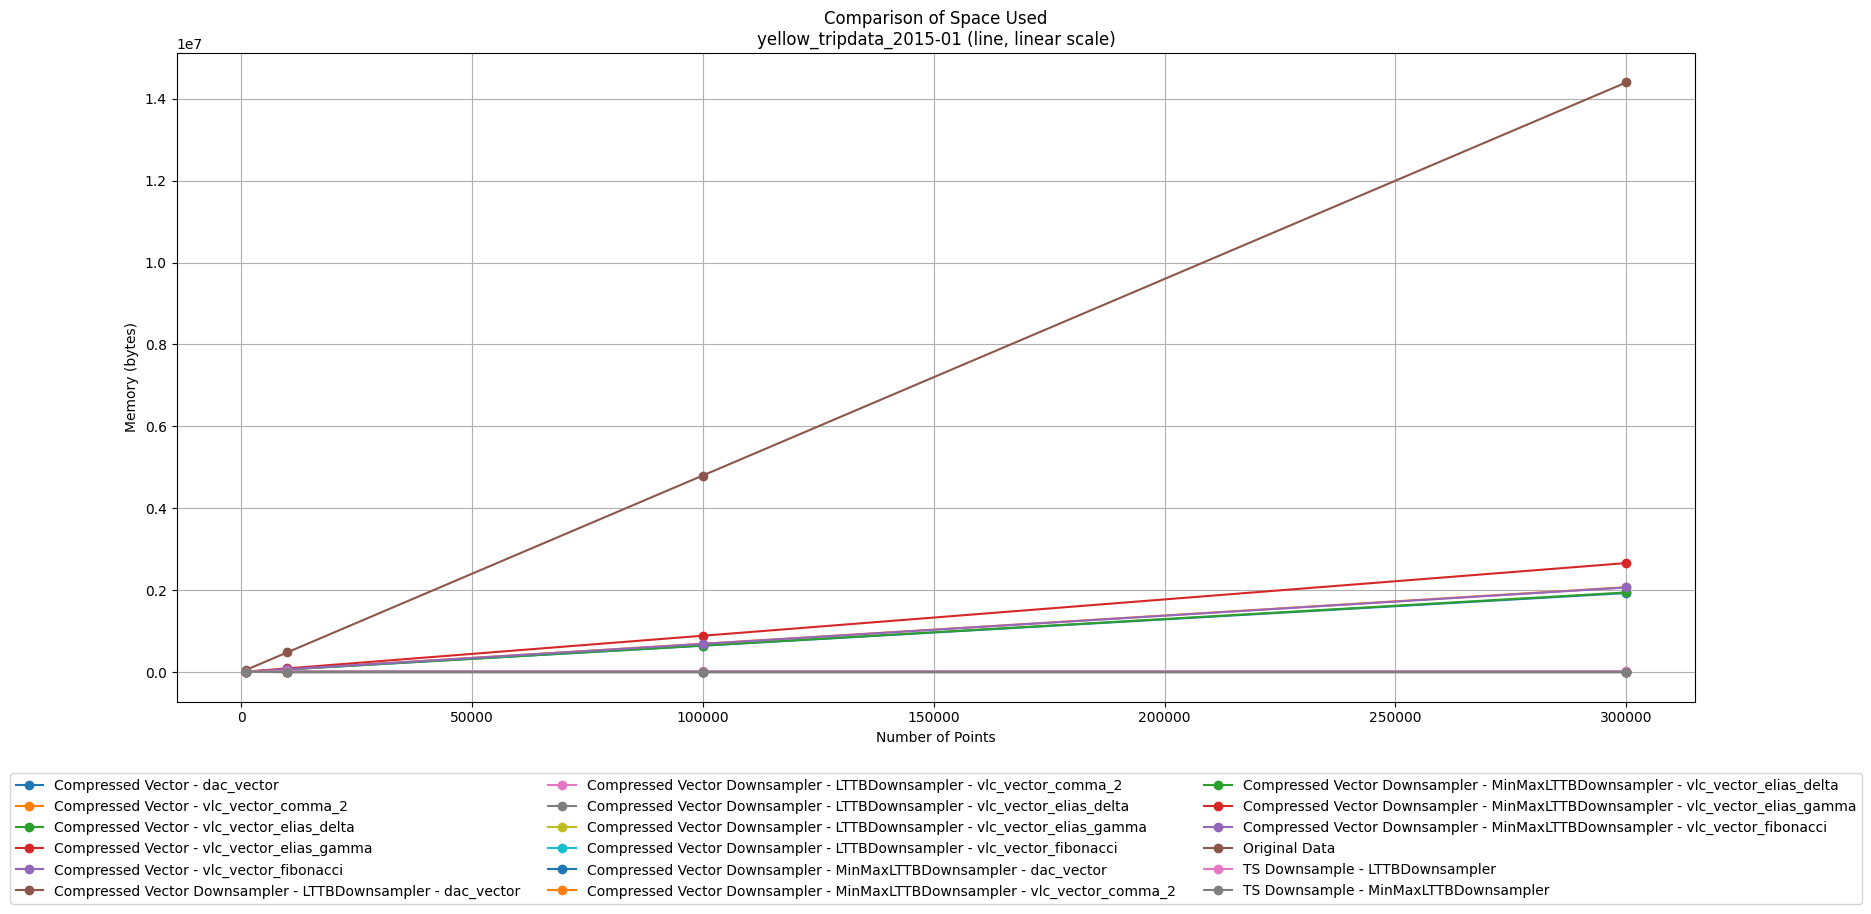
\includegraphics[width=1\textwidth]{anexo/exp/Comparison of Space Used/plots/Comparison of Space Used_yellow_tripdata_2015-01_linear_line.png}
        \caption[]{Gráfico de espacio usado por las diferentes bibliotecas para el input \textbf{yellow\_tripdata\_2015\_01}.}
        \label{fig:comparison_of_space_used_plot_line_3}
    \end{figure}
}

\DeclareRobustCommand{\ComparisonOfSpaceUsedThreePlotBar}{
    %insertar imagen
    \begin{figure}[H]
        \centering
        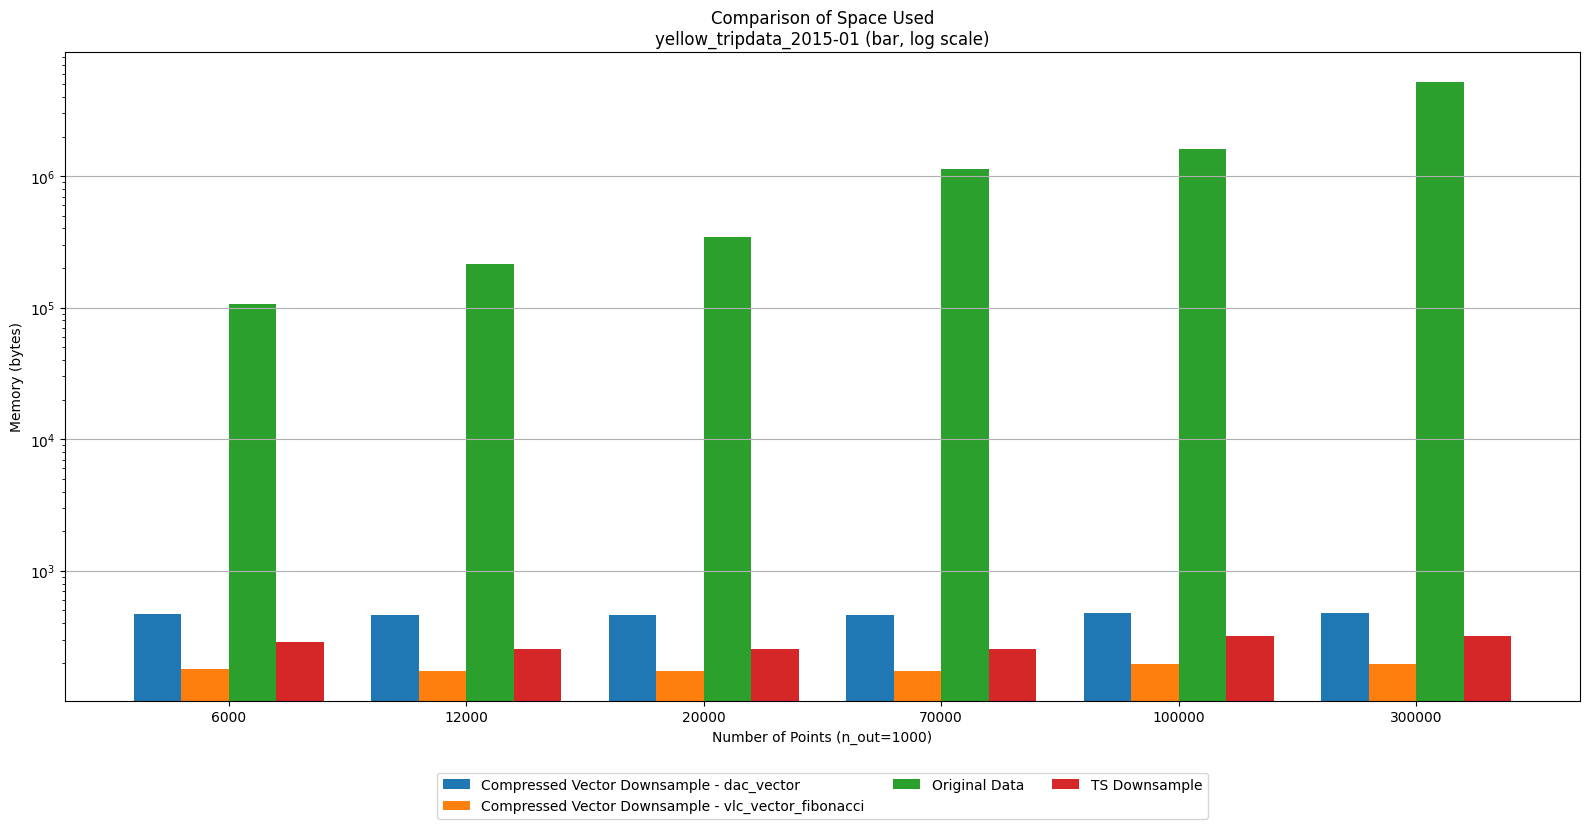
\includegraphics[width=1\textwidth]{anexo/exp/Comparison of Space Used/bar_plots/Comparison of Space Used_yellow_tripdata_2015-01_log_bar.png}
        \caption[]{Gráfico de espacio usado por las diferentes bibliotecas para el input \textbf{yellow\_tripdata\_2015\_01}.}
        \label{fig:comparison_of_space_used_plot_bar_3}
    \end{figure}
    \begin{table}[H]
        \centering
        \resizebox{\textwidth}{!}{%
        \begin{tabular}{|l|c|c|c|c|c|c|}
        \hline\multicolumn{1}{|c|}{Option} & \multicolumn{6}{c|}{\textbf{Number of data points}} \\
        \cline{2-7}
         & \textbf{6000} & \textbf{12000} & \textbf{20000} & \textbf{70000} & \textbf{100000} & \textbf{300000} \\
        \hline
        Compressed Vector Downsample - dac\_vector & 4.68e+02 [B] & 4.60e+02 [B] & 4.60e+02 [B] & 4.60e+02 [B] & 4.76e+02 [B] & 4.76e+02 [B] \\
        Compressed Vector Downsample - vlc\_vector\_fibonacci & 1.80e+02 [B] & 1.72e+02 [B] & 1.72e+02 [B] & 1.72e+02 [B] & 1.96e+02 [B] & 1.96e+02 [B] \\
        Original Data & 1.06e+05 [B] & 2.16e+05 [B] & 3.46e+05 [B] & 1.12e+06 [B] & 1.60e+06 [B] & 5.20e+06 [B] \\
        TS Downsample & 2.88e+02 [B] & 2.56e+02 [B] & 2.56e+02 [B] & 2.56e+02 [B] & 3.20e+02 [B] & 3.20e+02 [B] \\
        \hline
        \end{tabular}
        }
        \label{tab:comparison of space used-yellow-tripdata-2015-01}
    \end{table}
    \begin{table}[H]
\centering
\caption{Comparison of Space Used\_yellow\_tripdata\_2015-01 – Tasa de compactación CVD vs TS vs Datos Originales}
\label{tab:Comparison of Space Used\_yellow\_tripdata\_2015-01_cvd_compactacion}
\begin{tabular}{rlrr}
\toprule
n\_size & Variante & Comp. vs TS (\%) & Comp. vs Original (\%) \\
\midrule
6000 & CVD - dac\_vector & -62.50 & 99.56 \\
6000 & CVD - vlc\_vector\_fibonacci & 37.50 & 99.83 \\
12000 & CVD - dac\_vector & -79.69 & 99.79 \\
12000 & CVD - vlc\_vector\_fibonacci & 32.81 & 99.92 \\
20000 & CVD - dac\_vector & -79.69 & 99.87 \\
20000 & CVD - vlc\_vector\_fibonacci & 32.81 & 99.95 \\
70000 & CVD - dac\_vector & -79.69 & 99.96 \\
70000 & CVD - vlc\_vector\_fibonacci & 32.81 & 99.98 \\
100000 & CVD - dac\_vector & -48.75 & 99.97 \\
100000 & CVD - vlc\_vector\_fibonacci & 38.75 & 99.99 \\
300000 & CVD - dac\_vector & -48.75 & 99.99 \\
300000 & CVD - vlc\_vector\_fibonacci & 38.75 & 100.00 \\
\bottomrule
\end{tabular}

\end{table}
}



% ===========================
% CVD Decimal Places Access Time Comparison
% ===========================
\DeclareRobustCommand{\CVDDecimalPlacesAccessTimeComparisonOnePlotLine}{
    \begin{figure}[H]
        \centering
        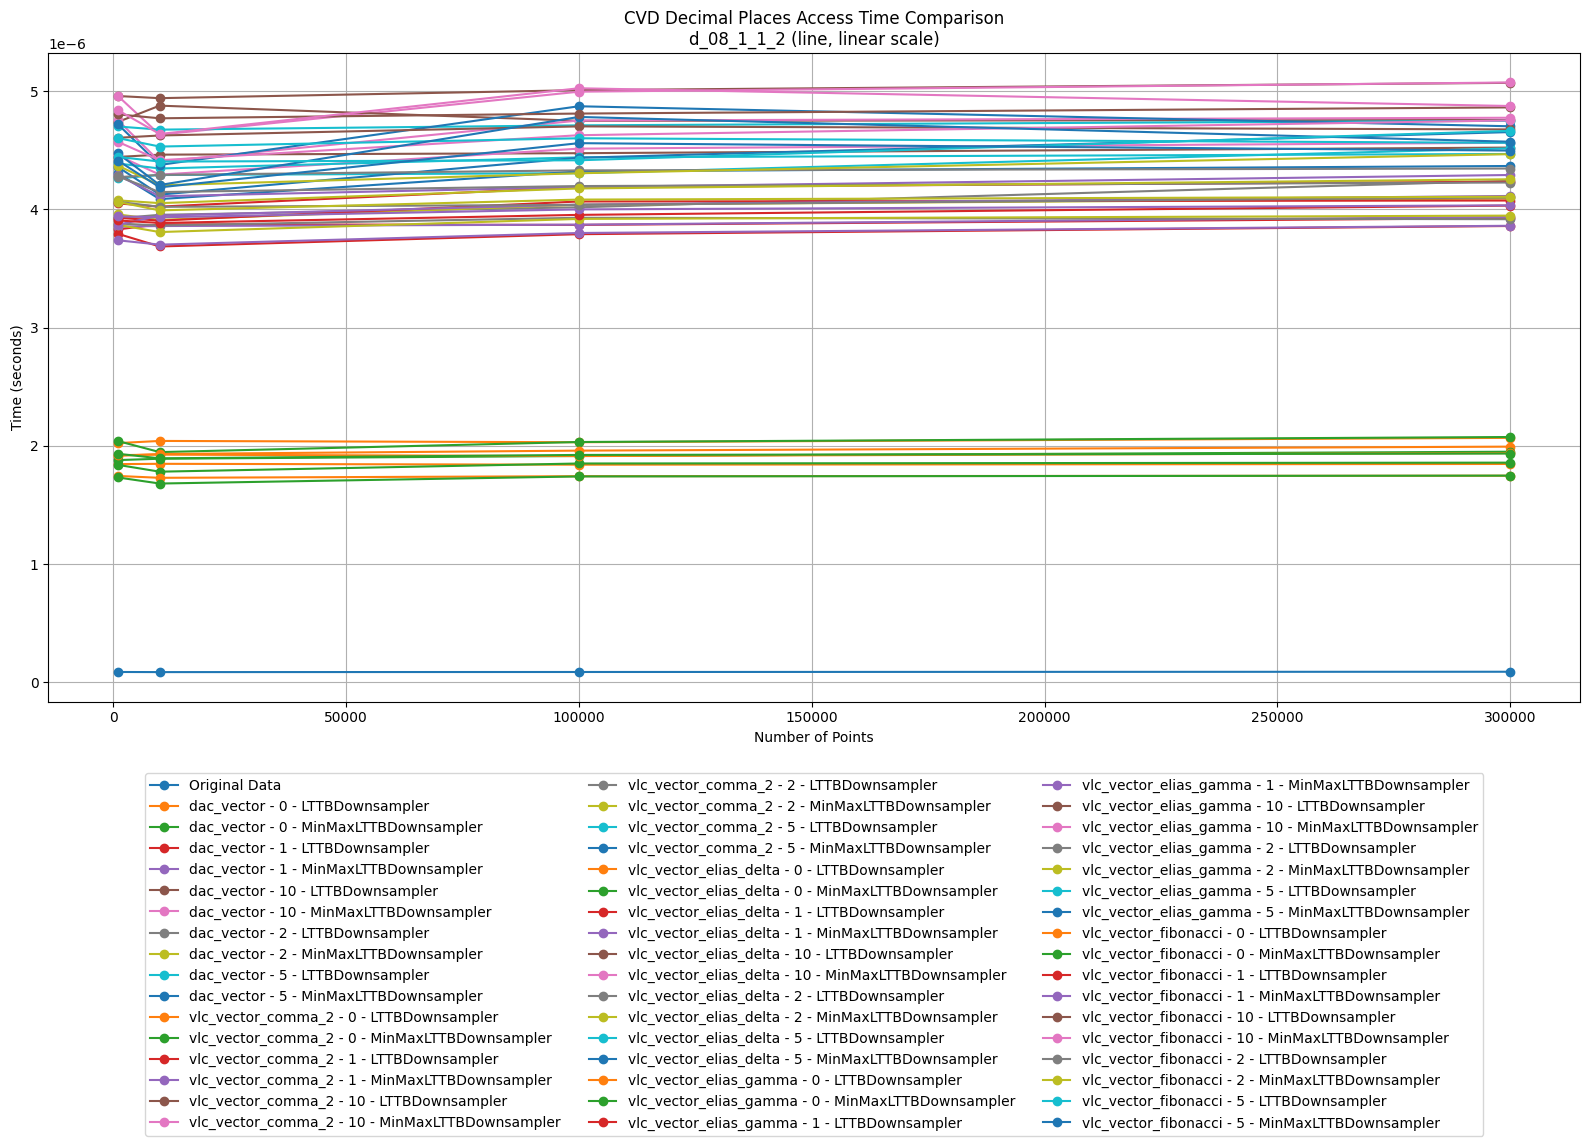
\includegraphics[width=1\textwidth]{anexo/exp/CVD Decimal Places Access Time Comparison/plots/CVD Decimal Places Access Time Comparison_d_08_1_1_2_linear_line.png}
        \caption[]{Gráfico de tiempo de acceso CVD con diferentes lugares decimales para el input \textbf{d\_08\_1\_1\_2}.}
        \label{fig:cvd_decimal_places_access_time_comparison_plot_line_1}
    \end{figure}
    \begin{figure}[H]
        \centering
        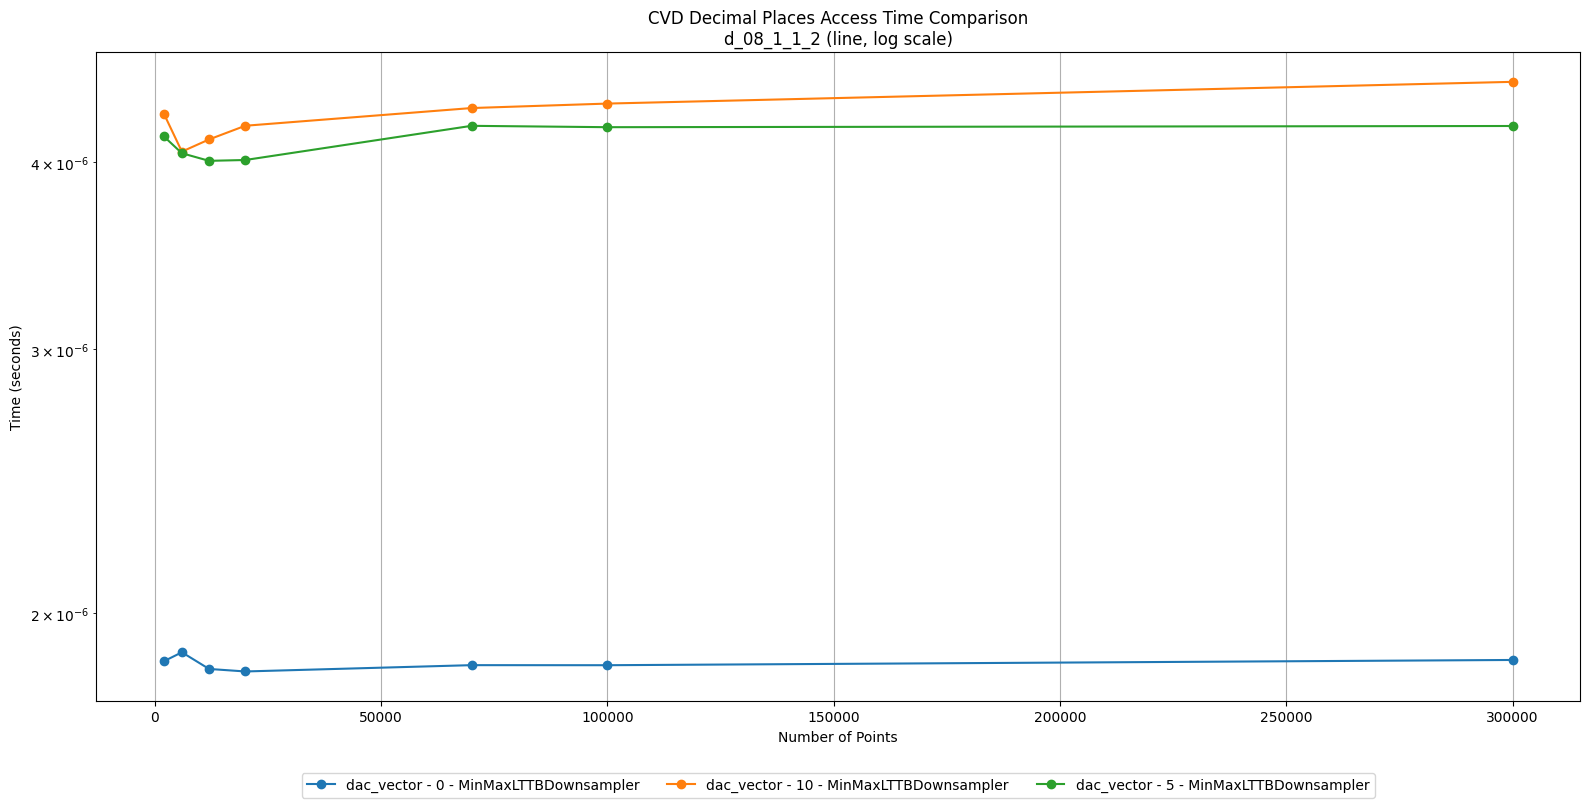
\includegraphics[width=1\textwidth]{anexo/exp/CVD Decimal Places Access Time Comparison/plots/CVD Decimal Places Access Time Comparison_d_08_1_1_2_log_line.png}
        \caption[]{Gráfico de tiempo de acceso CVD con diferentes lugares decimales para el input \textbf{d\_08\_1\_1\_2} en escala logarítmica.}
        \label{fig:cvd_decimal_places_access_time_comparison_plot_log_1}
    \end{figure}
}

\DeclareRobustCommand{\CVDDecimalPlacesAccessTimeComparisonTwoPlotLine}{
    \begin{figure}[H]
        \centering
        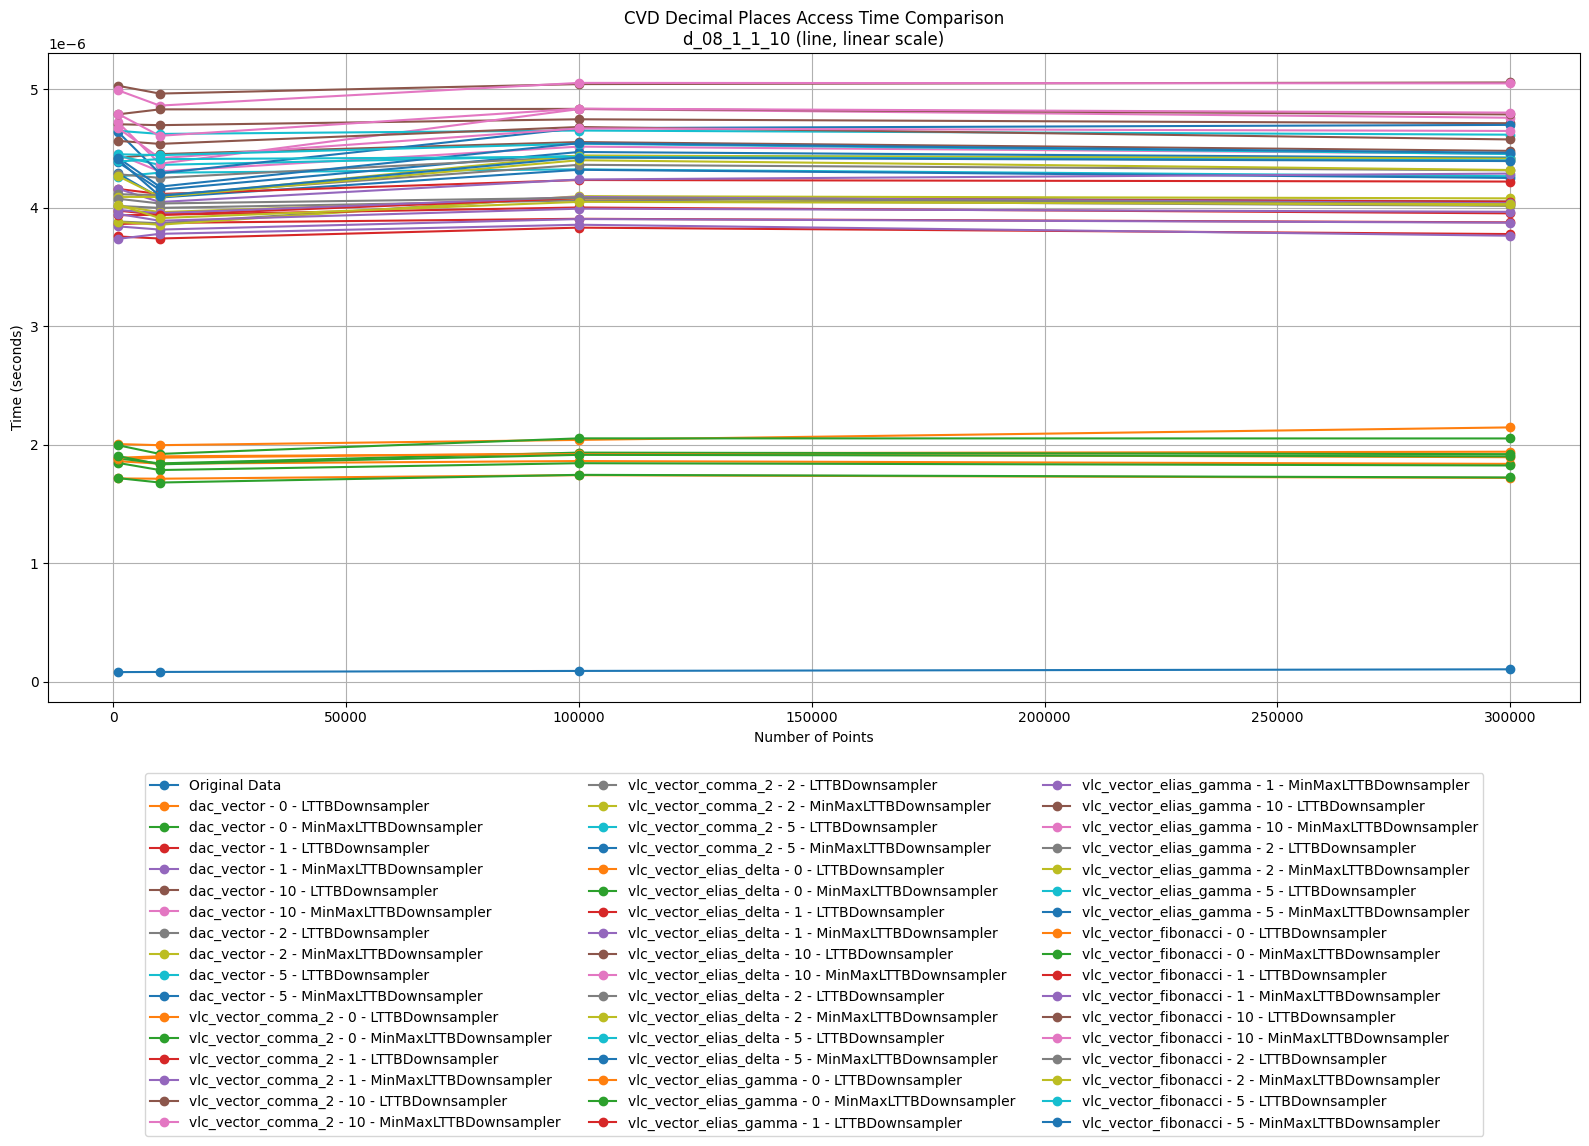
\includegraphics[width=1\textwidth]{anexo/exp/CVD Decimal Places Access Time Comparison/plots/CVD Decimal Places Access Time Comparison_d_08_1_1_10_linear_line.png}
        \caption[]{Gráfico de tiempo de acceso CVD con diferentes lugares decimales para el input \textbf{d\_08\_1\_1\_10}.}
        \label{fig:cvd_decimal_places_access_time_comparison_plot_line_2}
    \end{figure}
    \begin{figure}[H]
        \centering
        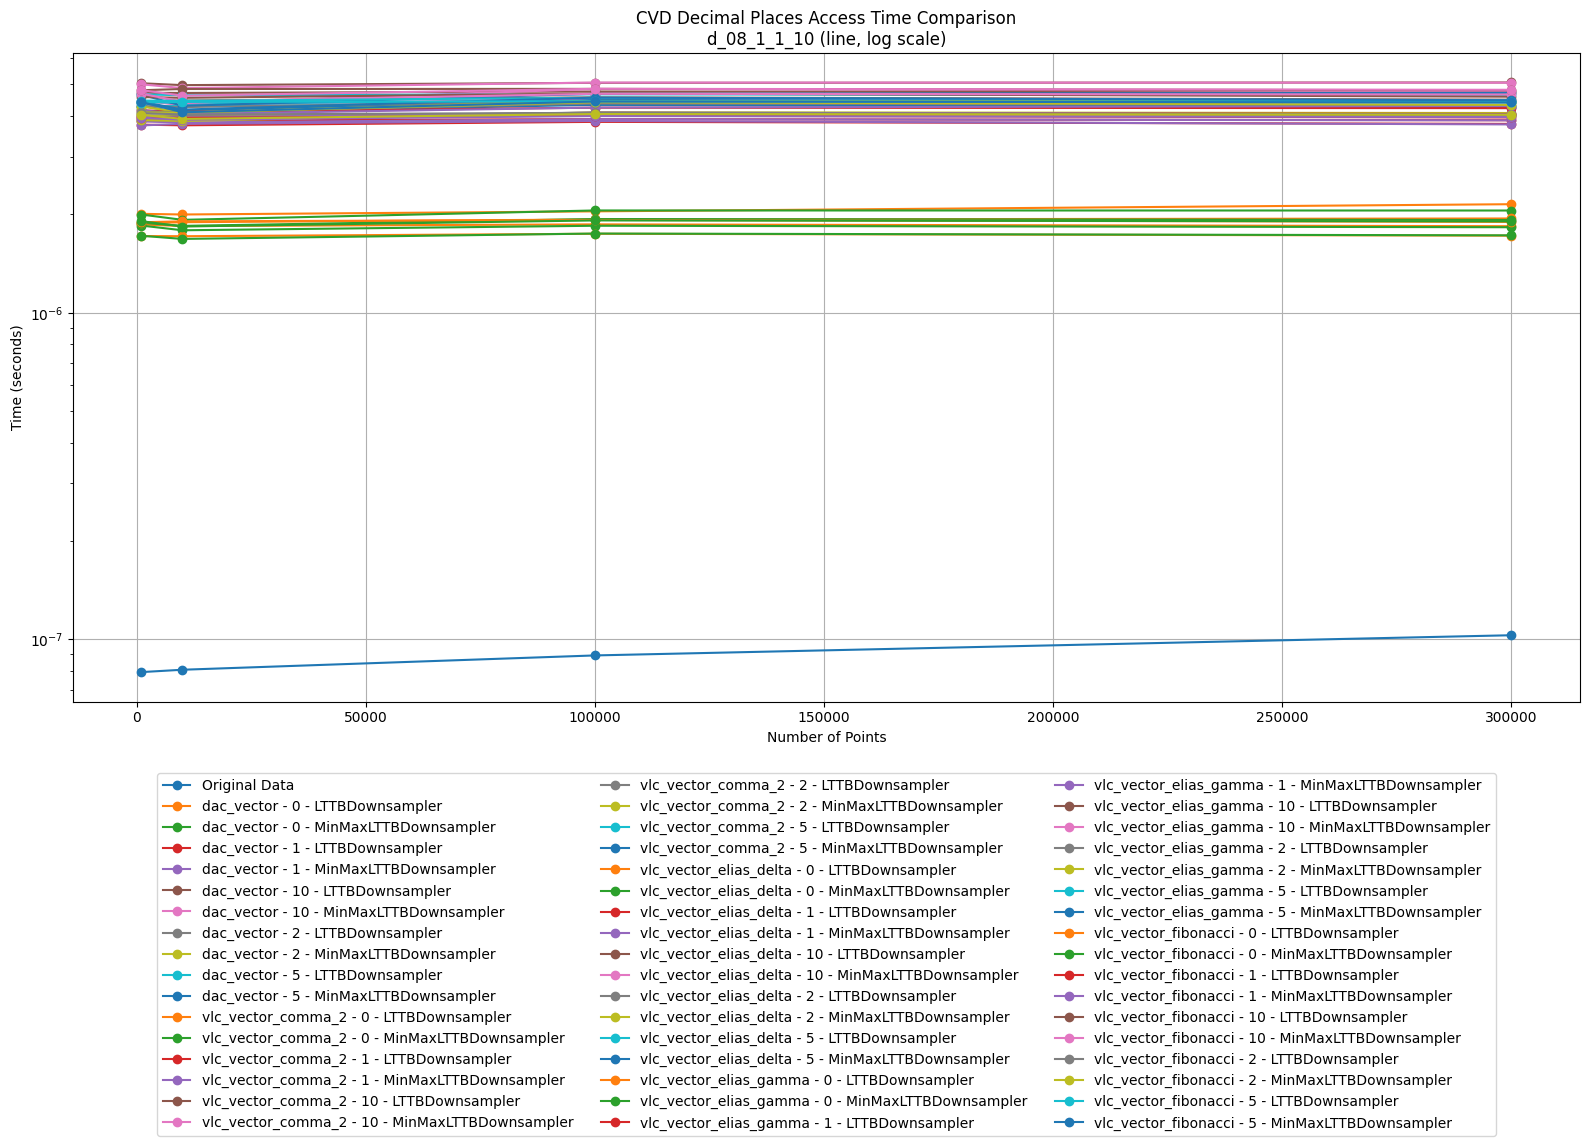
\includegraphics[width=1\textwidth]{anexo/exp/CVD Decimal Places Access Time Comparison/plots/CVD Decimal Places Access Time Comparison_d_08_1_1_10_log_line.png}
        \caption[]{Gráfico de tiempo de acceso CVD con diferentes lugares decimales para el input \textbf{d\_08\_1\_1\_10} en escala logarítmica.}
        \label{fig:cvd_decimal_places_access_time_comparison_plot_log_2}
    \end{figure}
}

\DeclareRobustCommand{\CVDDecimalPlacesAccessTimeComparisonThreePlotLine}{
    \begin{figure}[H]
        \centering
        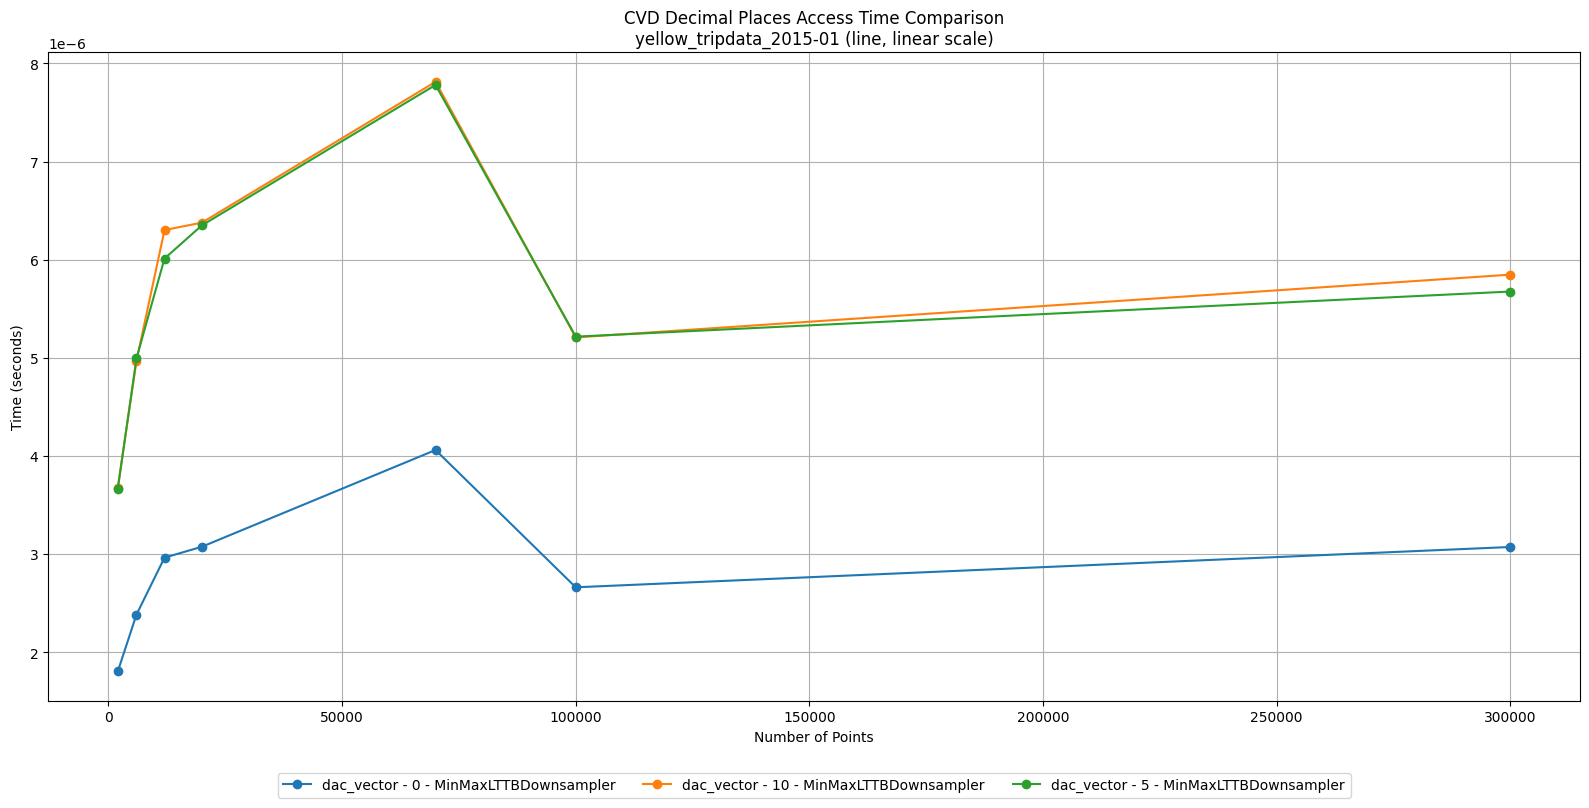
\includegraphics[width=1\textwidth]{anexo/exp/CVD Decimal Places Access Time Comparison/plots/CVD Decimal Places Access Time Comparison_yellow_tripdata_2015-01_linear_line.png}
        \caption[]{Gráfico de tiempo de acceso CVD con diferentes lugares decimales para el input \textbf{yellow\_tripdata\_2015\_01}.}
        \label{fig:cvd_decimal_places_access_time_comparison_plot_line_3}
    \end{figure}
    \begin{figure}[H]
        \centering
        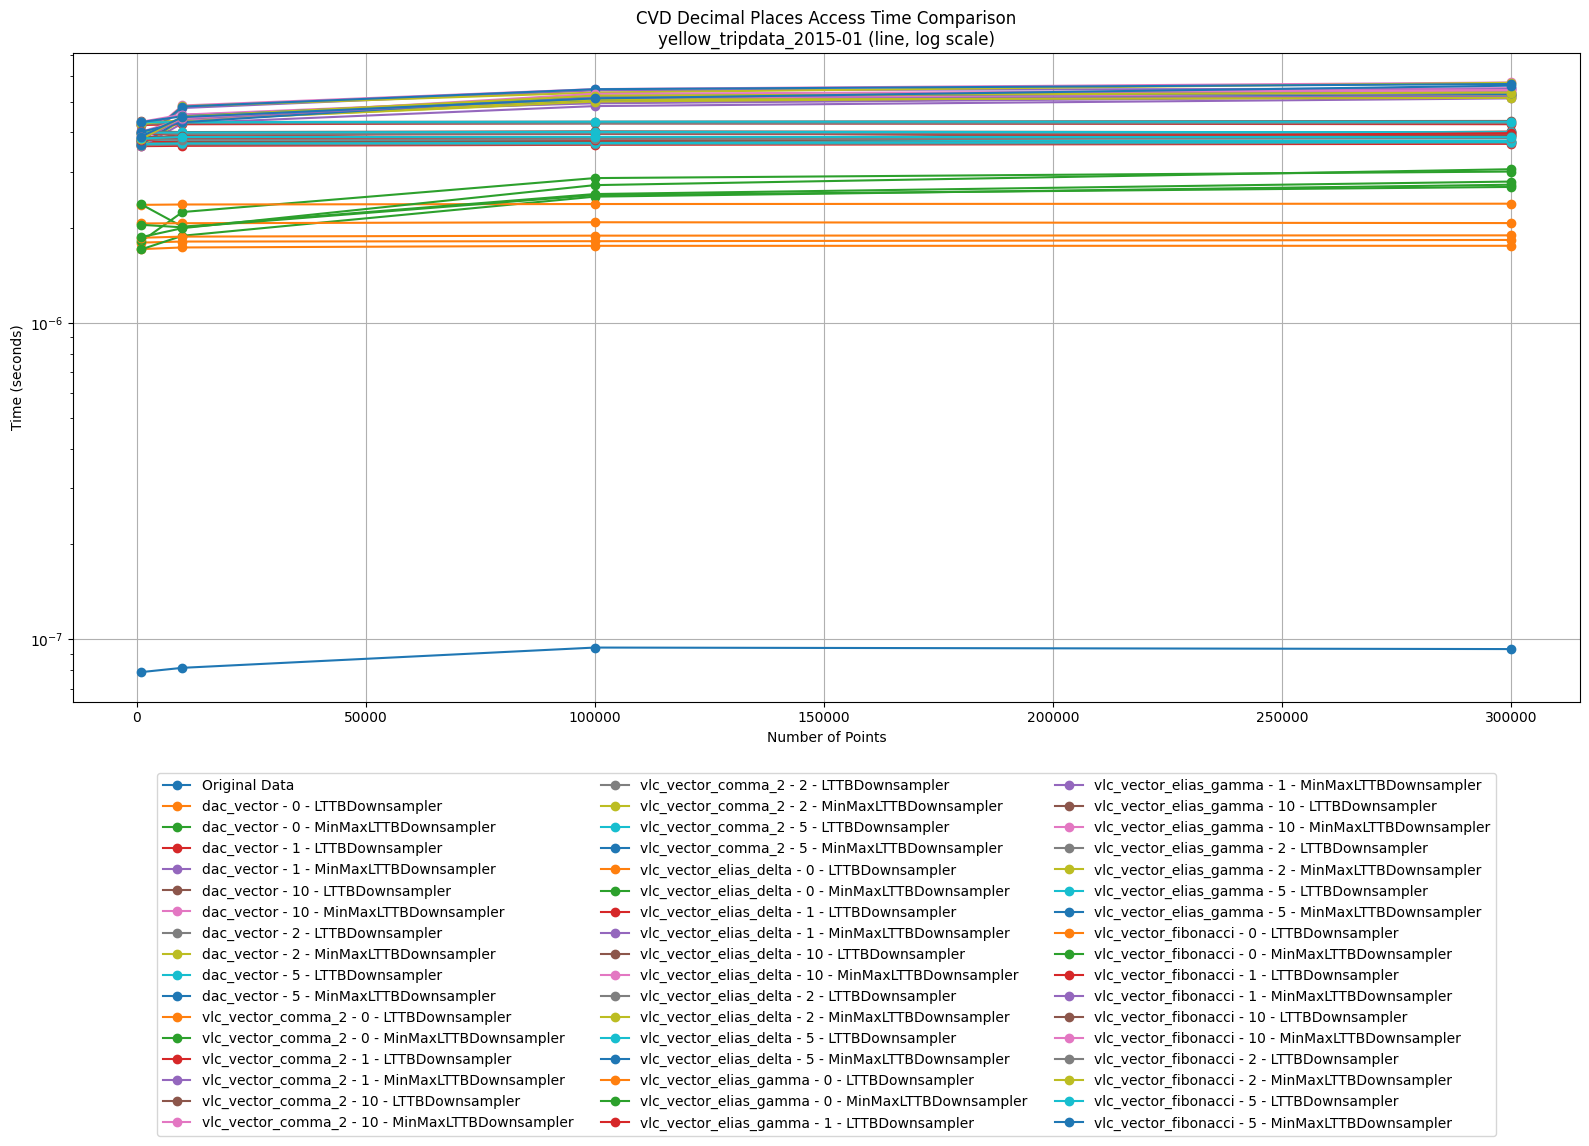
\includegraphics[width=1\textwidth]{anexo/exp/CVD Decimal Places Access Time Comparison/plots/CVD Decimal Places Access Time Comparison_yellow_tripdata_2015-01_log_line.png}
        \caption[]{Gráfico de tiempo de acceso CVD con diferentes lugares decimales para el input \textbf{yellow\_tripdata\_2015\_01} en escala logarítmica.}
        \label{fig:cvd_decimal_places_access_time_comparison_plot_log_3}
    \end{figure}
}


% ===========================
% CVD Decimal Places Build Time Comparison
% ===========================
\DeclareRobustCommand{\CVDDecimalPlacesBuildTimeComparisonOnePlotLine}{
    \begin{figure}[H]
        \centering
        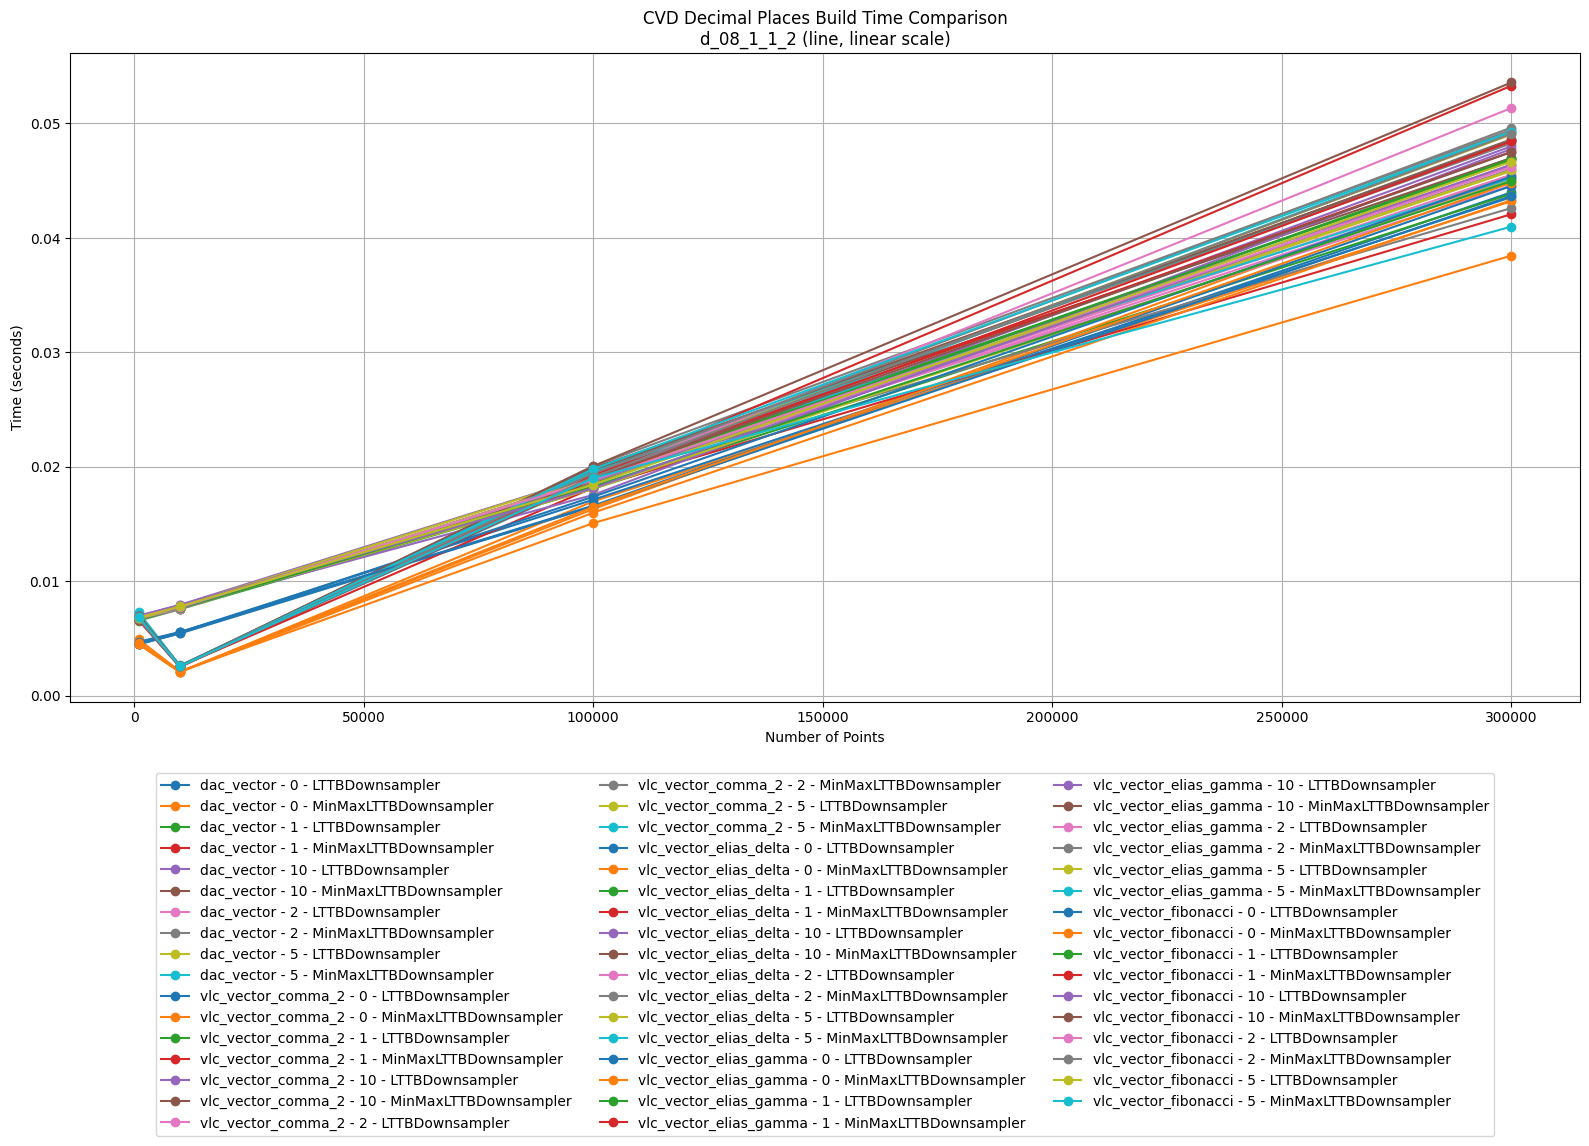
\includegraphics[width=1\textwidth]{anexo/exp/CVD Decimal Places Build Time Comparison/plots/CVD Decimal Places Build Time Comparison_d_08_1_1_2_linear_line.png}
        \caption[]{Gráfico de tiempo de construcción CVD con diferentes lugares decimales para el input \textbf{d\_08\_1\_1\_2}.}
        \label{fig:cvd_decimal_places_build_time_comparison_plot_line_1}
    \end{figure}
    \begin{figure}[H]
        \centering
        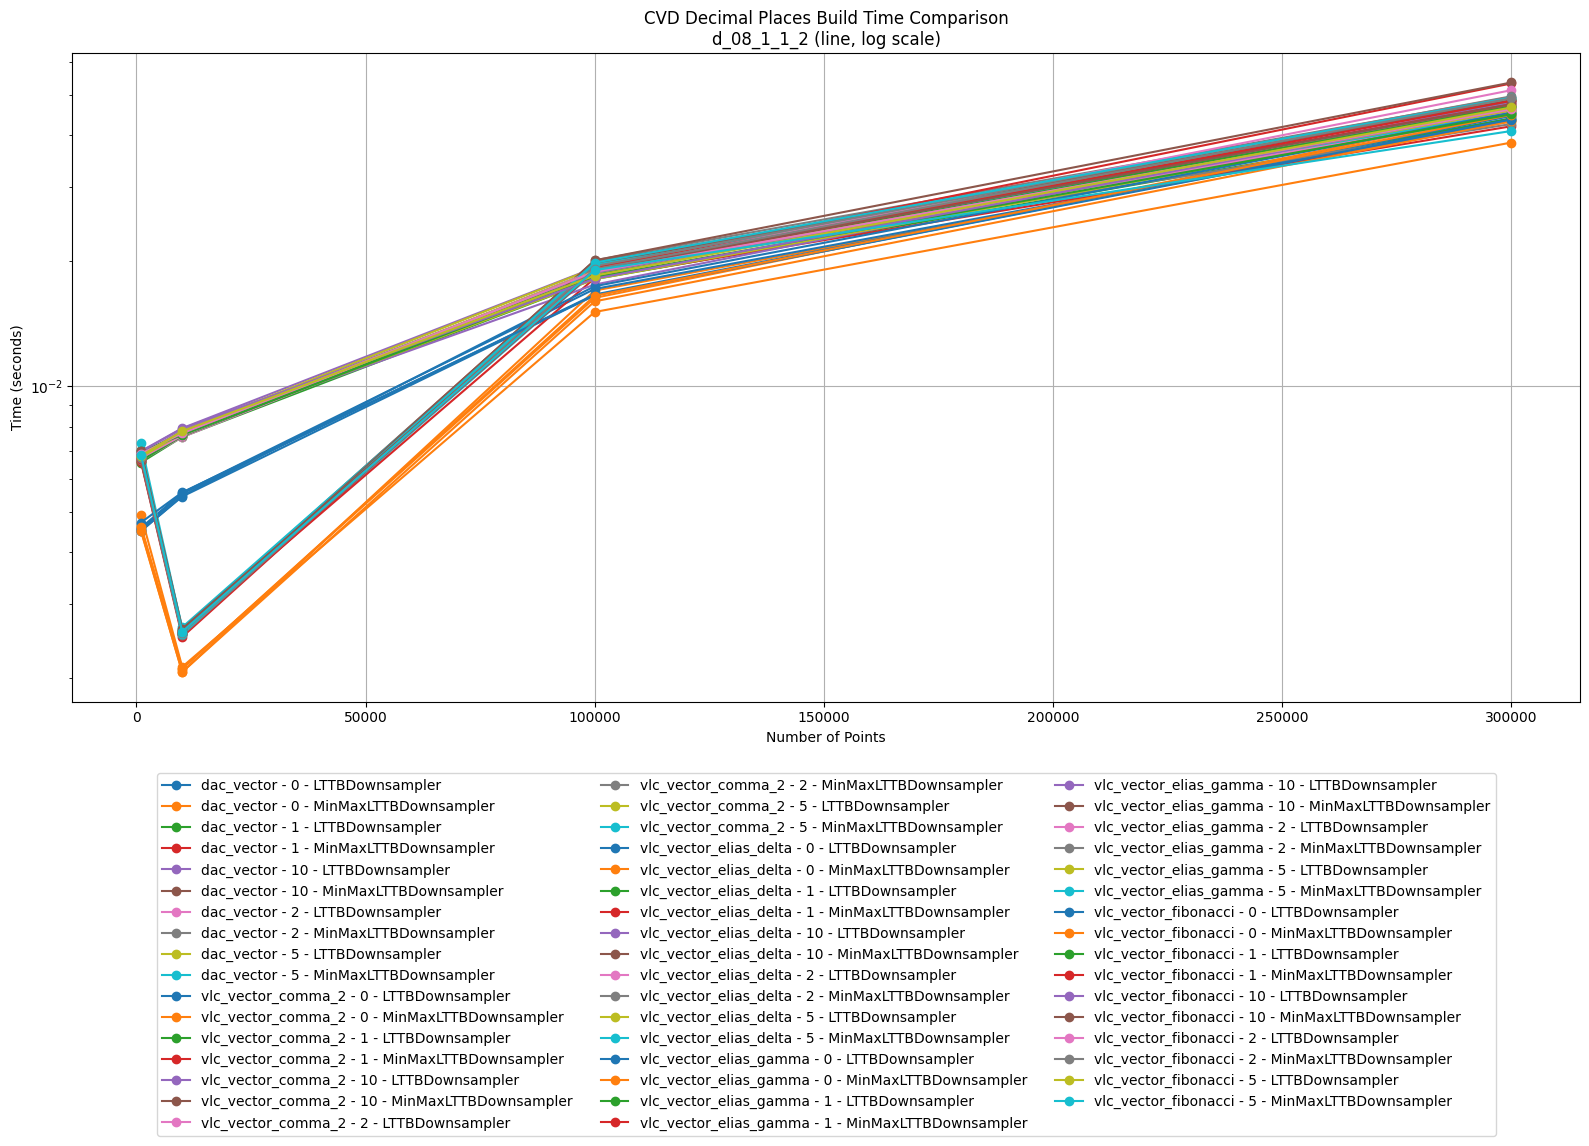
\includegraphics[width=1\textwidth]{anexo/exp/CVD Decimal Places Build Time Comparison/plots/CVD Decimal Places Build Time Comparison_d_08_1_1_2_log_line.png}
        \caption[]{Gráfico de tiempo de construcción CVD con diferentes lugares decimales para el input \textbf{d\_08\_1\_1\_2} en escala logarítmica.}
        \label{fig:cvd_decimal_places_build_time_comparison_plot_log_1}
    \end{figure}
}

\DeclareRobustCommand{\CVDDecimalPlacesBuildTimeComparisonTwoPlotLine}{
    \begin{figure}[H]
        \centering
        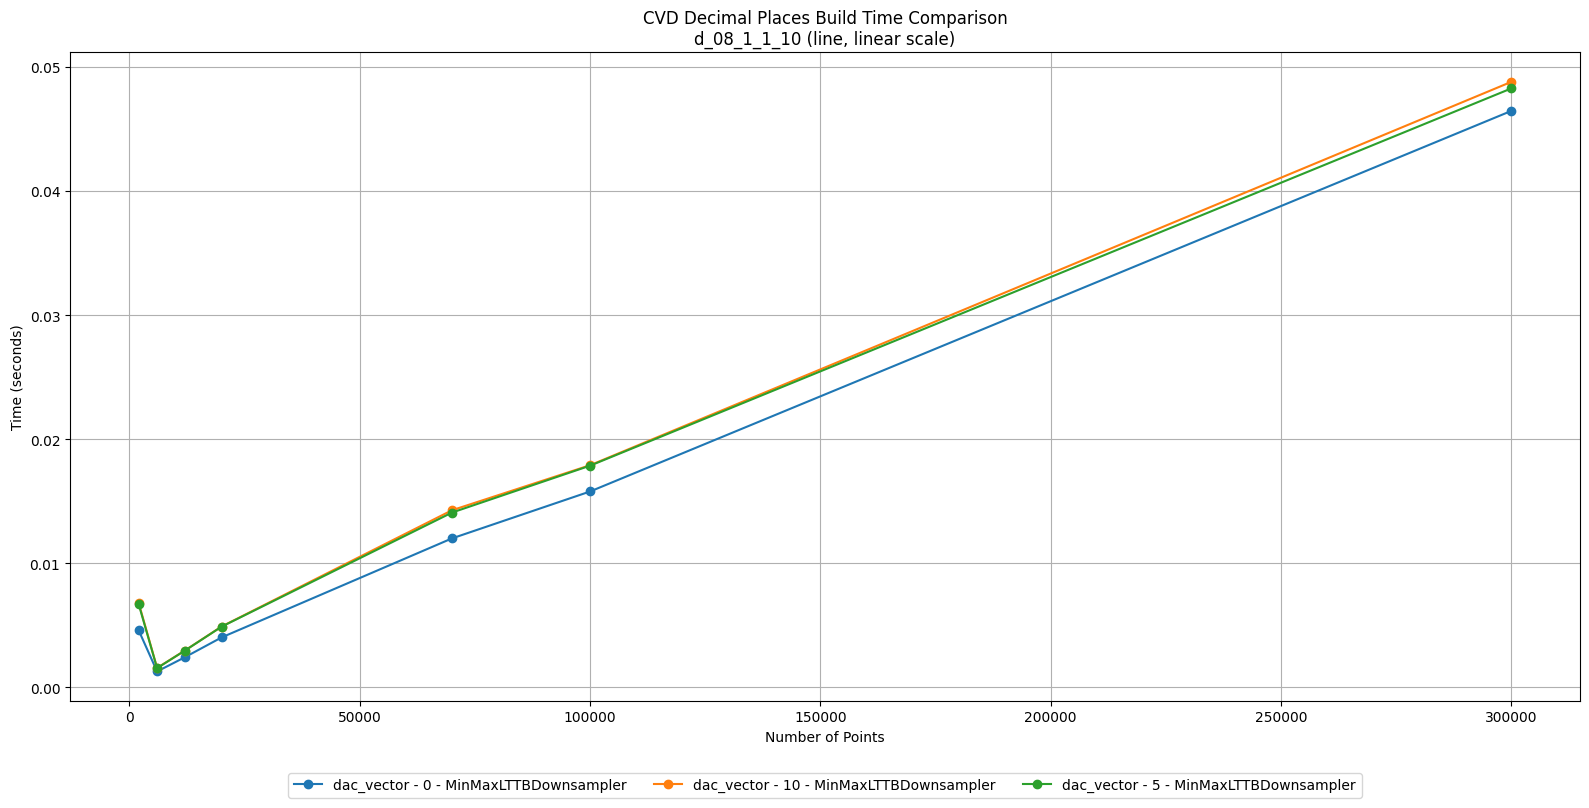
\includegraphics[width=1\textwidth]{anexo/exp/CVD Decimal Places Build Time Comparison/plots/CVD Decimal Places Build Time Comparison_d_08_1_1_10_linear_line.png}
        \caption[]{Gráfico de tiempo de construcción CVD con diferentes lugares decimales para el input \textbf{d\_08\_1\_1\_10}.}
        \label{fig:cvd_decimal_places_build_time_comparison_plot_line_2}
    \end{figure}
    \begin{figure}[H]
        \centering
        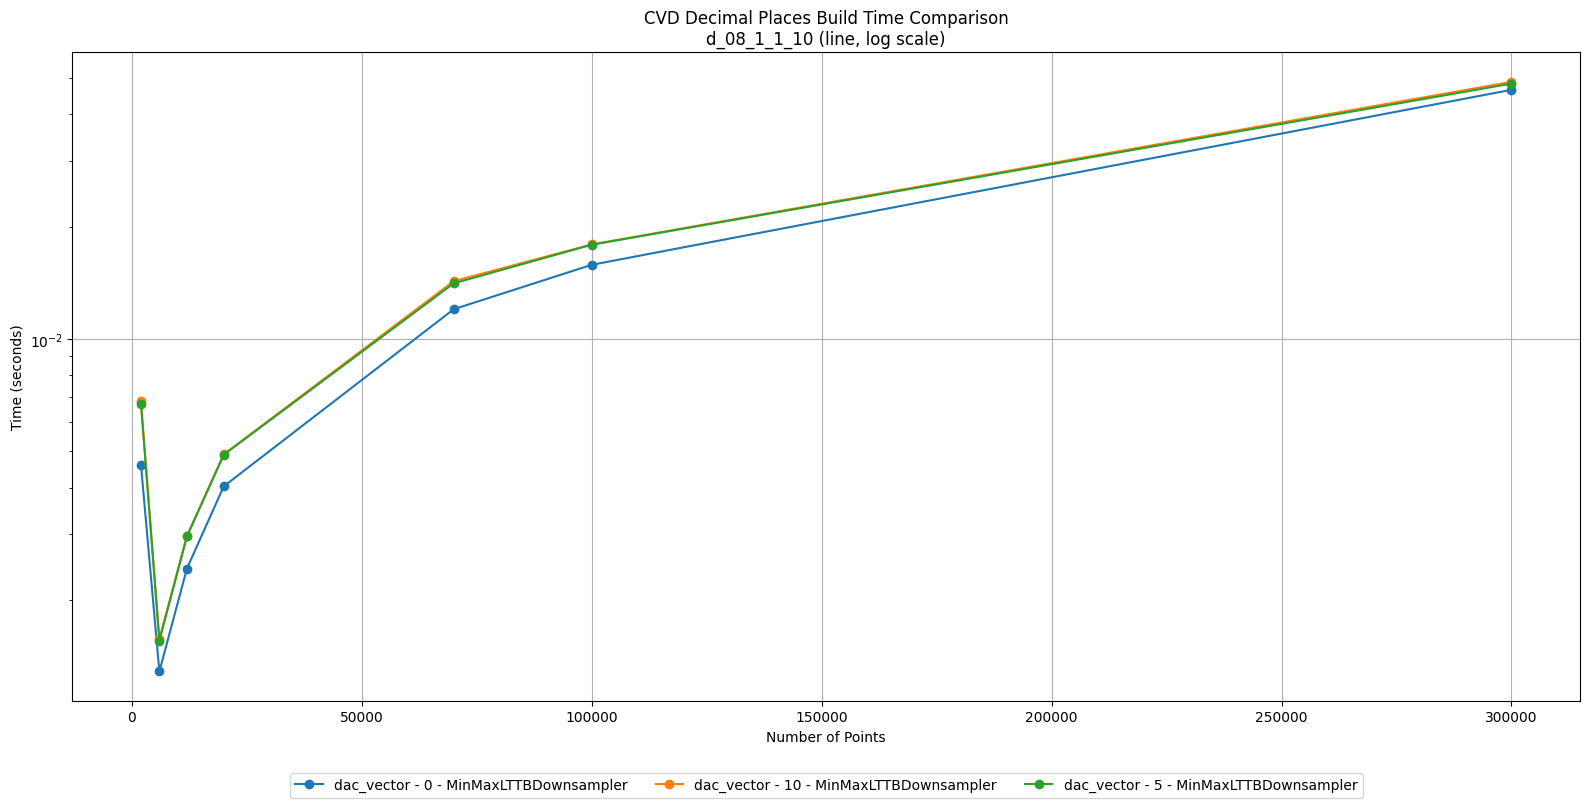
\includegraphics[width=1\textwidth]{anexo/exp/CVD Decimal Places Build Time Comparison/plots/CVD Decimal Places Build Time Comparison_d_08_1_1_10_log_line.png}
        \caption[]{Gráfico de tiempo de construcción CVD con diferentes lugares decimales para el input \textbf{d\_08\_1\_1\_10} en escala logarítmica.}
        \label{fig:cvd_decimal_places_build_time_comparison_plot_log_2}
    \end{figure}
}

\DeclareRobustCommand{\CVDDecimalPlacesBuildTimeComparisonThreePlotLine}{
    \begin{figure}[H]
        \centering
        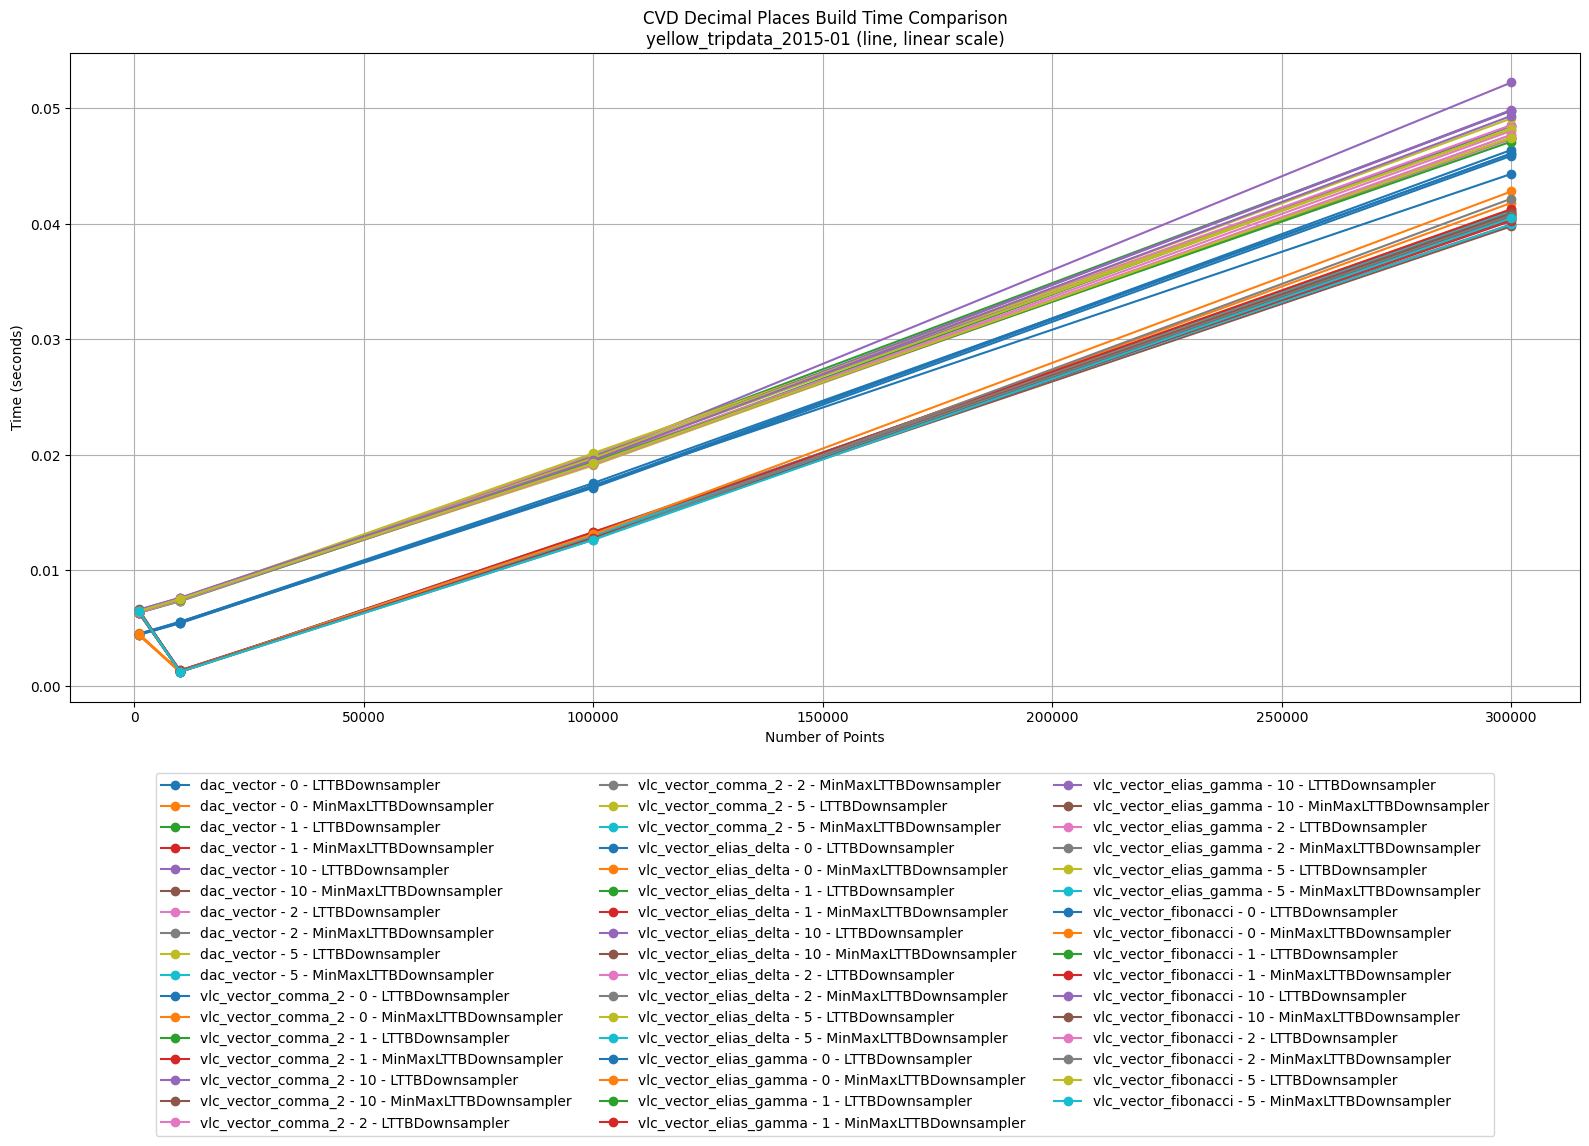
\includegraphics[width=1\textwidth]{anexo/exp/CVD Decimal Places Build Time Comparison/plots/CVD Decimal Places Build Time Comparison_yellow_tripdata_2015-01_linear_line.png}
        \caption[]{Gráfico de tiempo de construcción CVD con diferentes lugares decimales para el input \textbf{yellow\_tripdata\_2015\_01}.}
        \label{fig:cvd_decimal_places_build_time_comparison_plot_line_3}
    \end{figure}
    \begin{figure}[H]
        \centering
        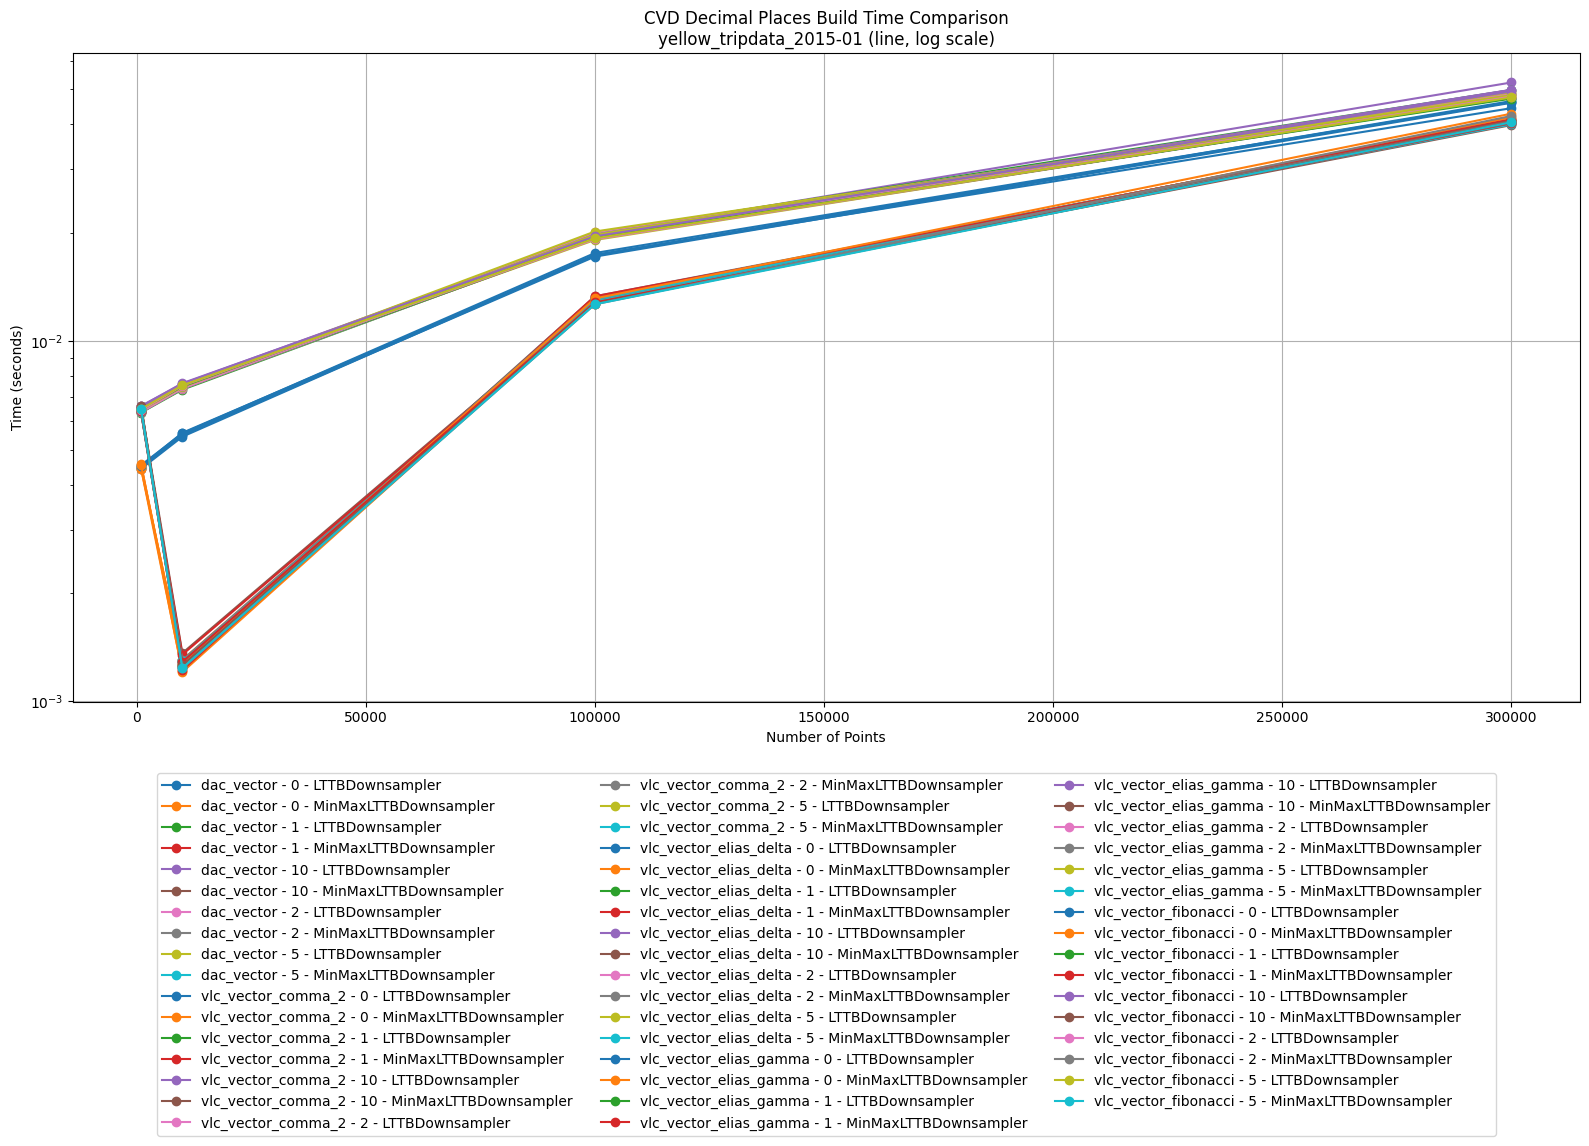
\includegraphics[width=1\textwidth]{anexo/exp/CVD Decimal Places Build Time Comparison/plots/CVD Decimal Places Build Time Comparison_yellow_tripdata_2015-01_log_line.png}
        \caption[]{Gráfico de tiempo de construcción CVD con diferentes lugares decimales para el input \textbf{yellow\_tripdata\_2015\_01} en escala logarítmica.}
        \label{fig:cvd_decimal_places_build_time_comparison_plot_log_3}
    \end{figure}
}


% ===========================
% CVD Decimal Places Size Comparison
% ===========================
\DeclareRobustCommand{\CVDDecimalPlacesSizeComparisonOnePlotLine}{
    \begin{figure}[H]
        \centering
        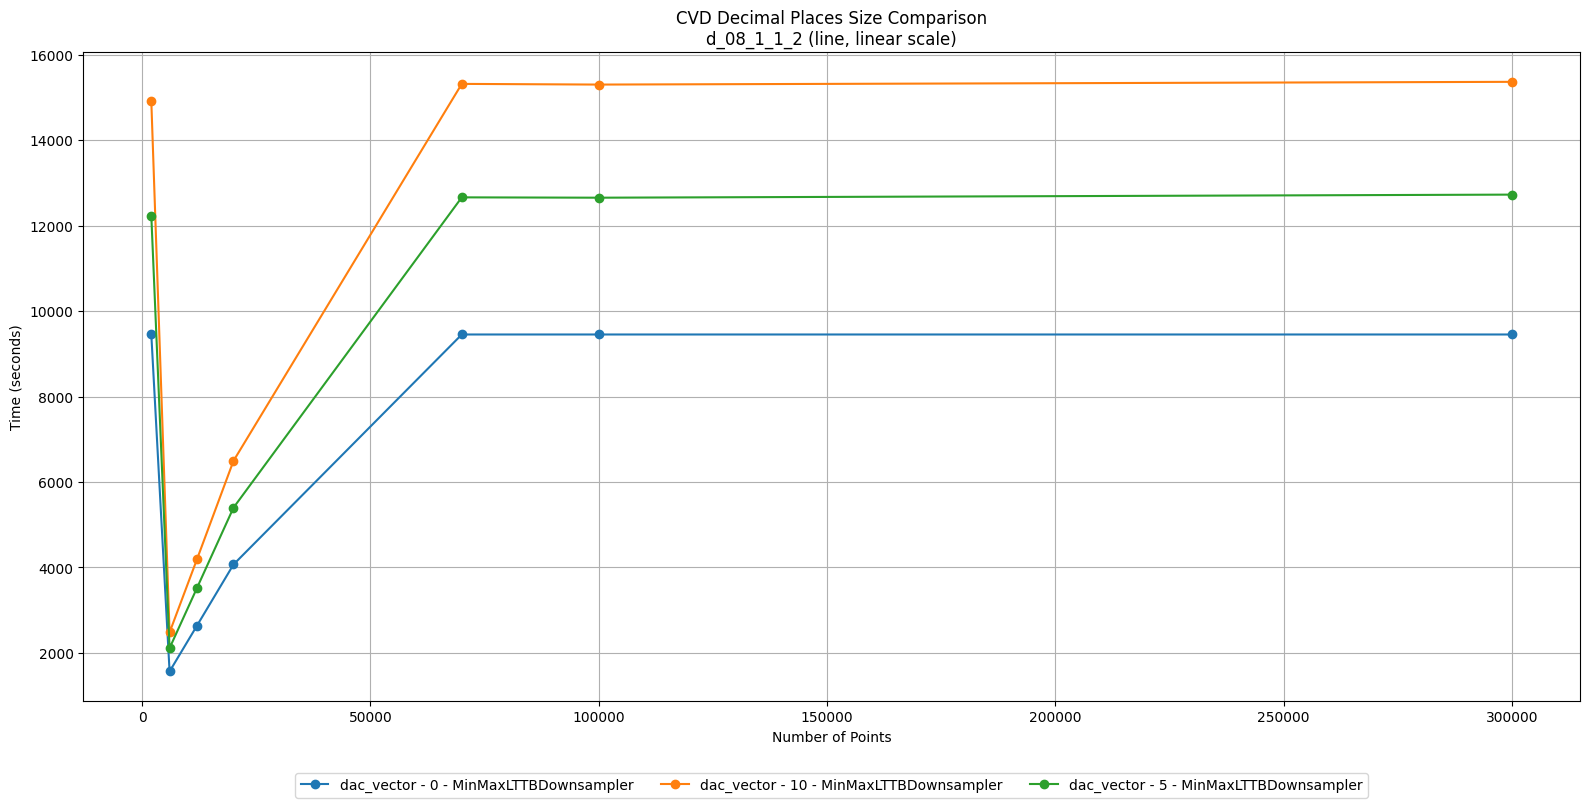
\includegraphics[width=1\textwidth]{anexo/exp/CVD Decimal Places Size Comparison/plots/CVD Decimal Places Size Comparison_d_08_1_1_2_linear_line.png}
        \caption[]{Gráfico de tamaño CVD con diferentes lugares decimales para el input \textbf{d\_08\_1\_1\_2}.}
        \label{fig:cvd_decimal_places_size_comparison_plot_line_1}
    \end{figure}
    \begin{figure}[H]
        \centering
        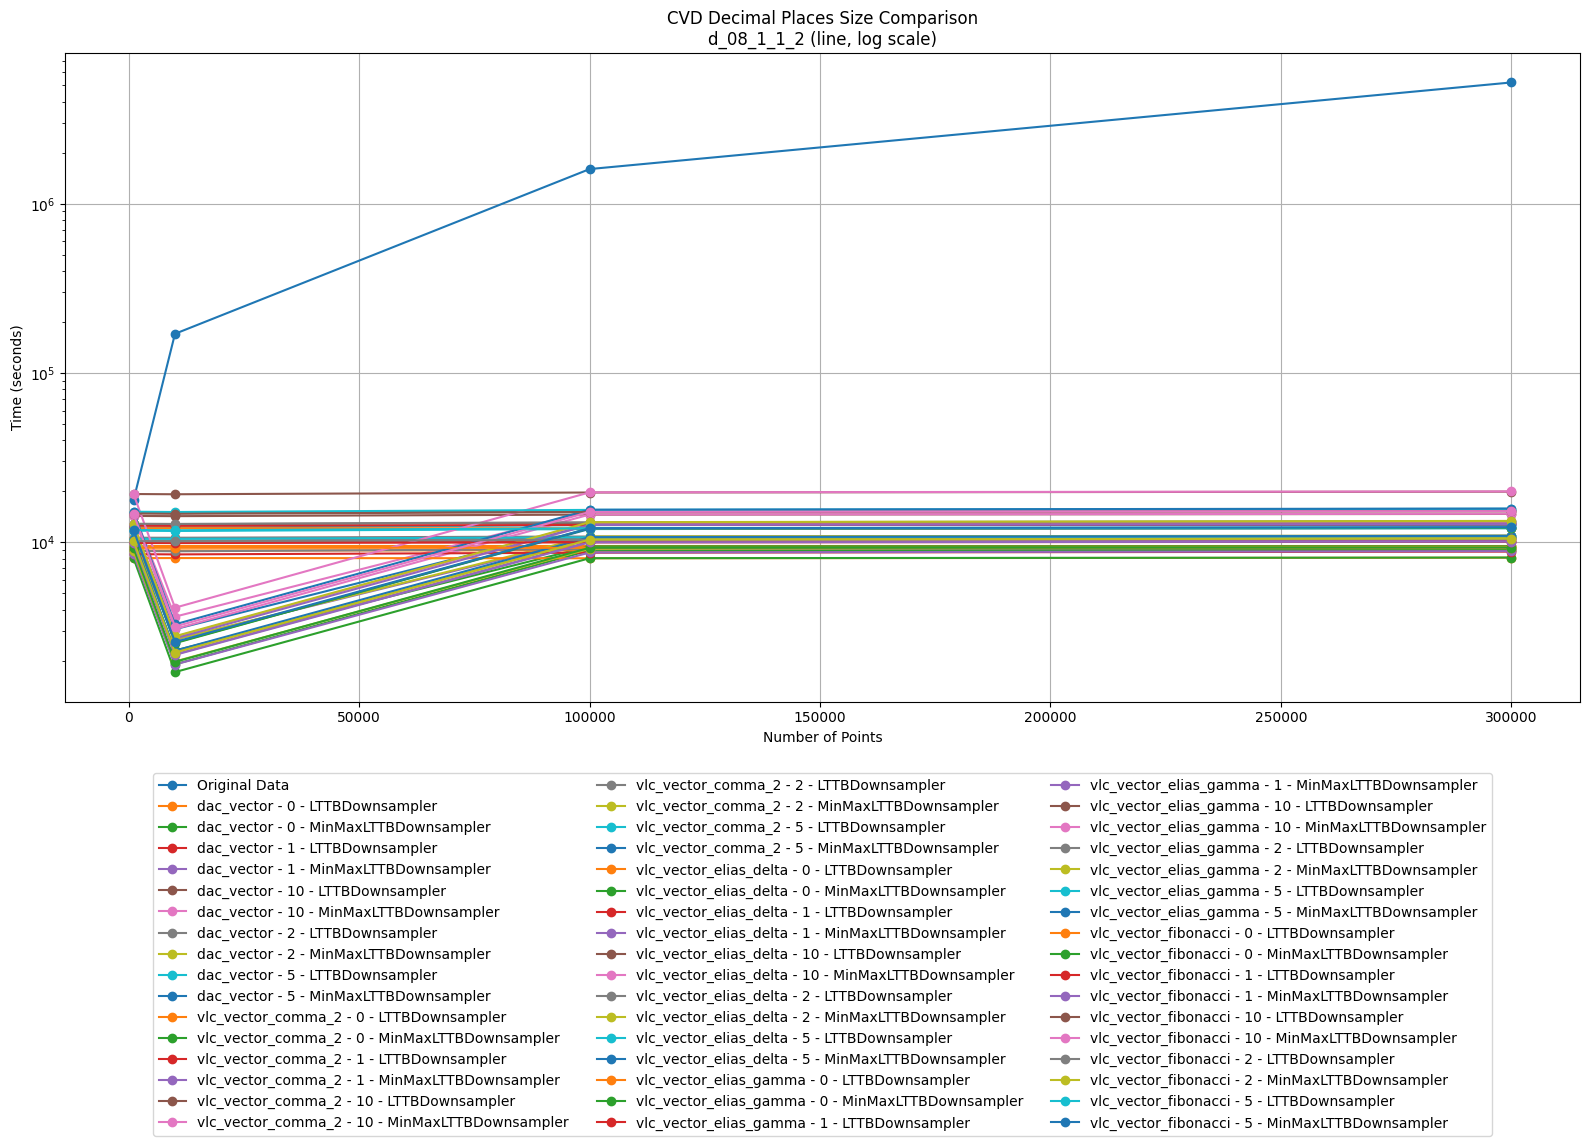
\includegraphics[width=1\textwidth]{anexo/exp/CVD Decimal Places Size Comparison/plots/CVD Decimal Places Size Comparison_d_08_1_1_2_log_line.png}
        \caption[]{Gráfico de tamaño CVD con diferentes lugares decimales para el input \textbf{d\_08\_1\_1\_2} en escala logarítmica.}
        \label{fig:cvd_decimal_places_size_comparison_plot_log_1}
    \end{figure}
}

\DeclareRobustCommand{\CVDDecimalPlacesSizeComparisonTwoPlotLine}{
    \begin{figure}[H]
        \centering
        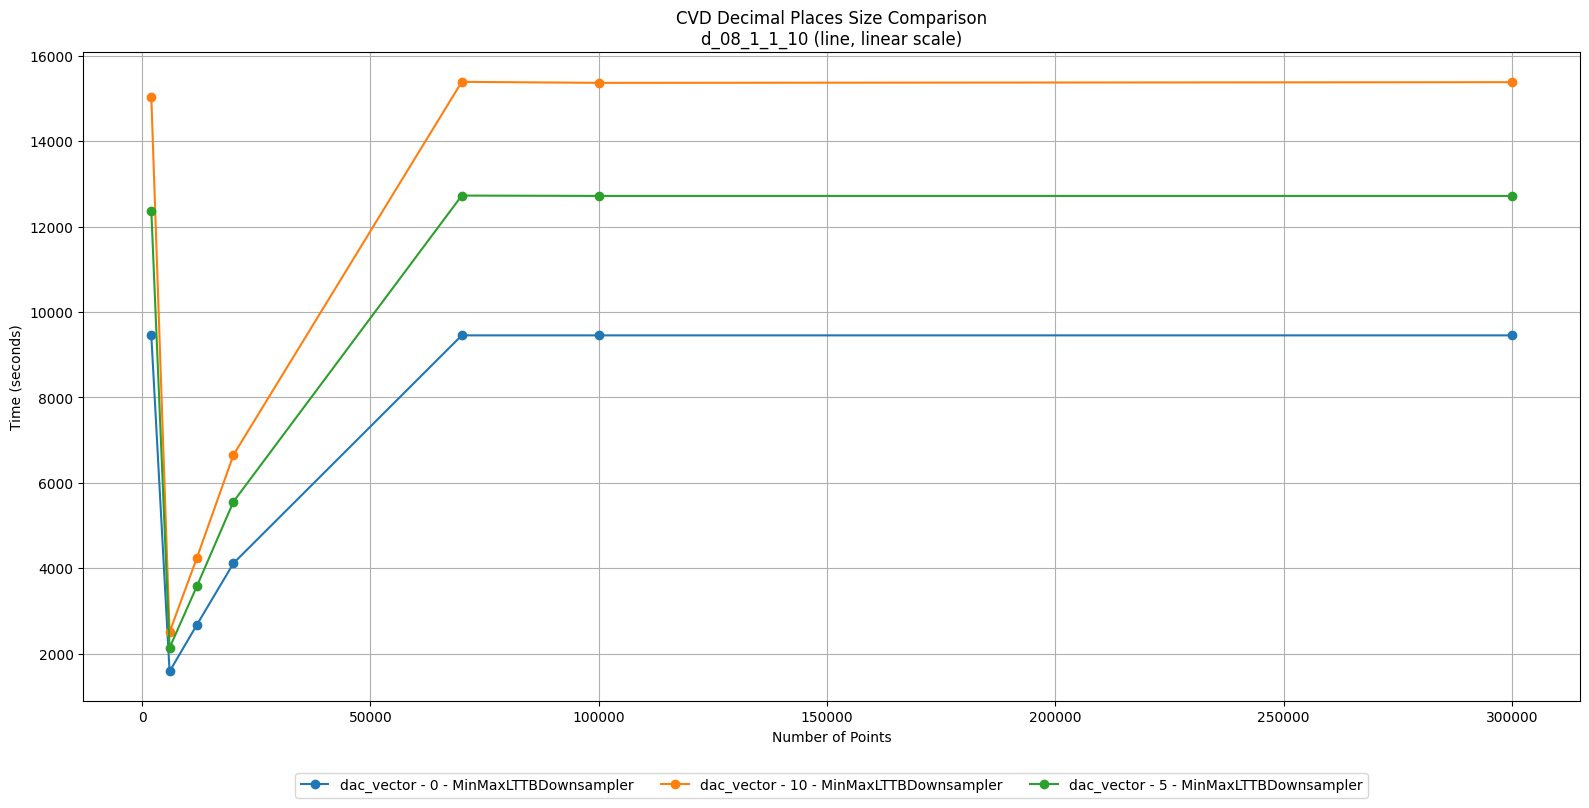
\includegraphics[width=1\textwidth]{anexo/exp/CVD Decimal Places Size Comparison/plots/CVD Decimal Places Size Comparison_d_08_1_1_10_linear_line.png}
        \caption[]{Gráfico de tamaño CVD con diferentes lugares decimales para el input \textbf{d\_08\_1\_1\_10}.}
        \label{fig:cvd_decimal_places_size_comparison_plot_line_2}
    \end{figure}
    \begin{figure}[H]
        \centering
        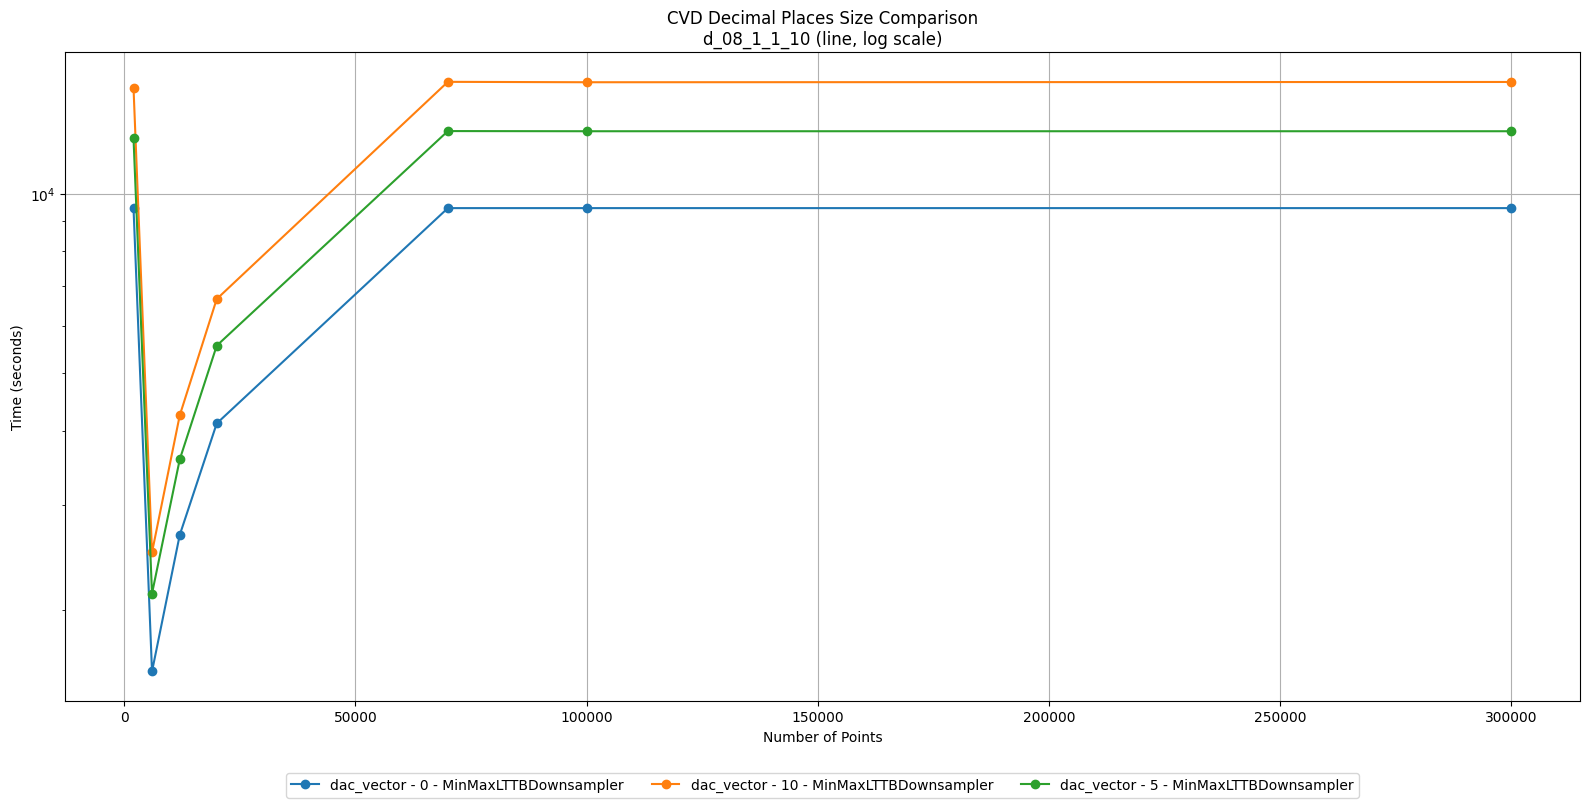
\includegraphics[width=1\textwidth]{anexo/exp/CVD Decimal Places Size Comparison/plots/CVD Decimal Places Size Comparison_d_08_1_1_10_log_line.png}
        \caption[]{Gráfico de tamaño CVD con diferentes lugares decimales para el input \textbf{d\_08\_1\_1\_10} en escala logarítmica.}
        \label{fig:cvd_decimal_places_size_comparison_plot_log_2}
    \end{figure}
}

\DeclareRobustCommand{\CVDDecimalPlacesSizeComparisonThreePlotLine}{
    \begin{figure}[H]
        \centering
        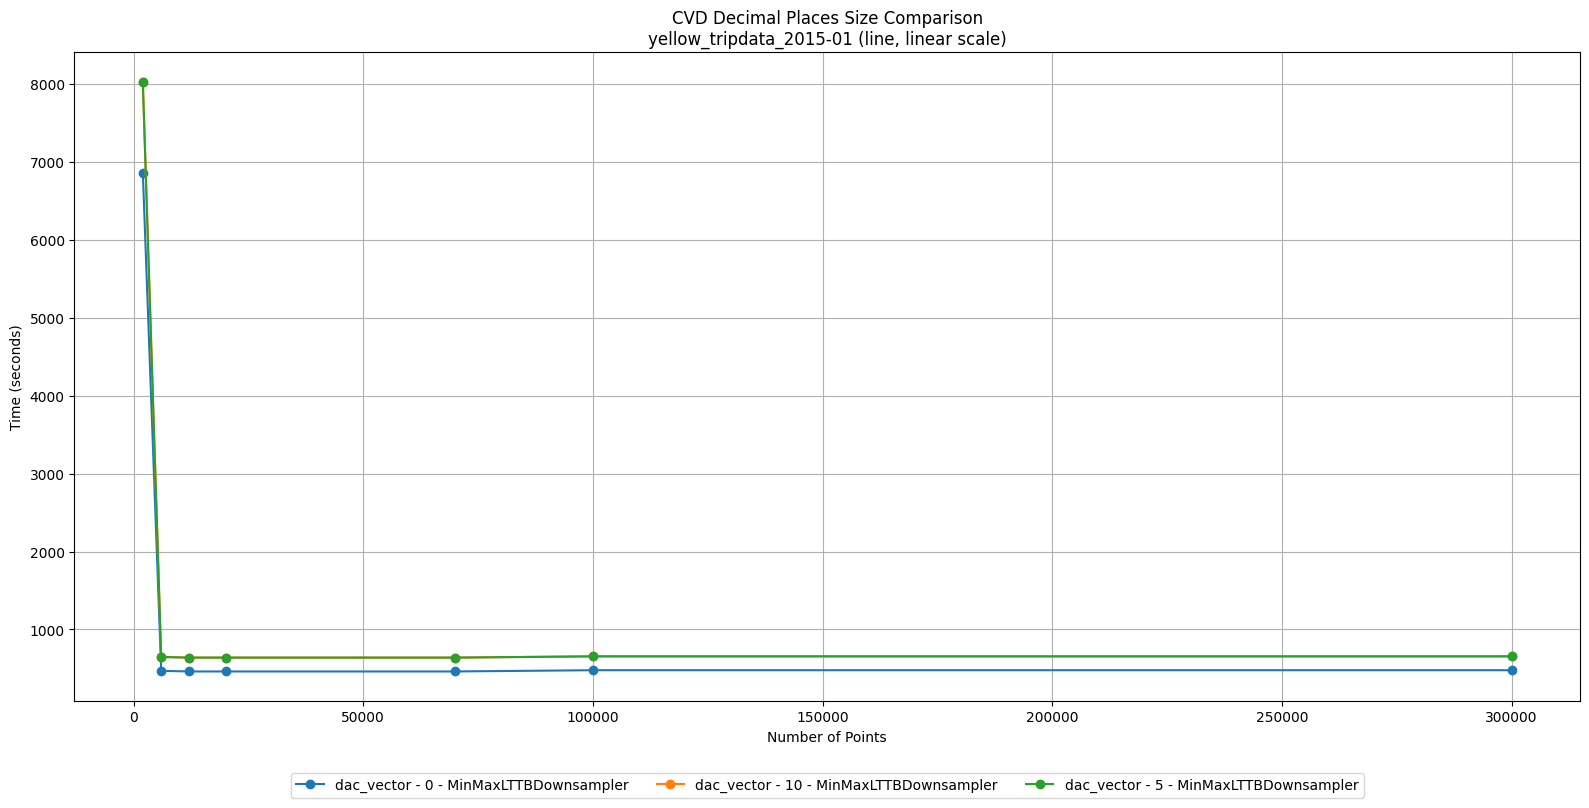
\includegraphics[width=1\textwidth]{anexo/exp/CVD Decimal Places Size Comparison/plots/CVD Decimal Places Size Comparison_yellow_tripdata_2015-01_linear_line.png}
        \caption[]{Gráfico de tamaño CVD con diferentes lugares decimales para el input \textbf{yellow\_tripdata\_2015\_01}.}
        \label{fig:cvd_decimal_places_size_comparison_plot_line_3}
    \end{figure}
    \begin{figure}[H]
        \centering
        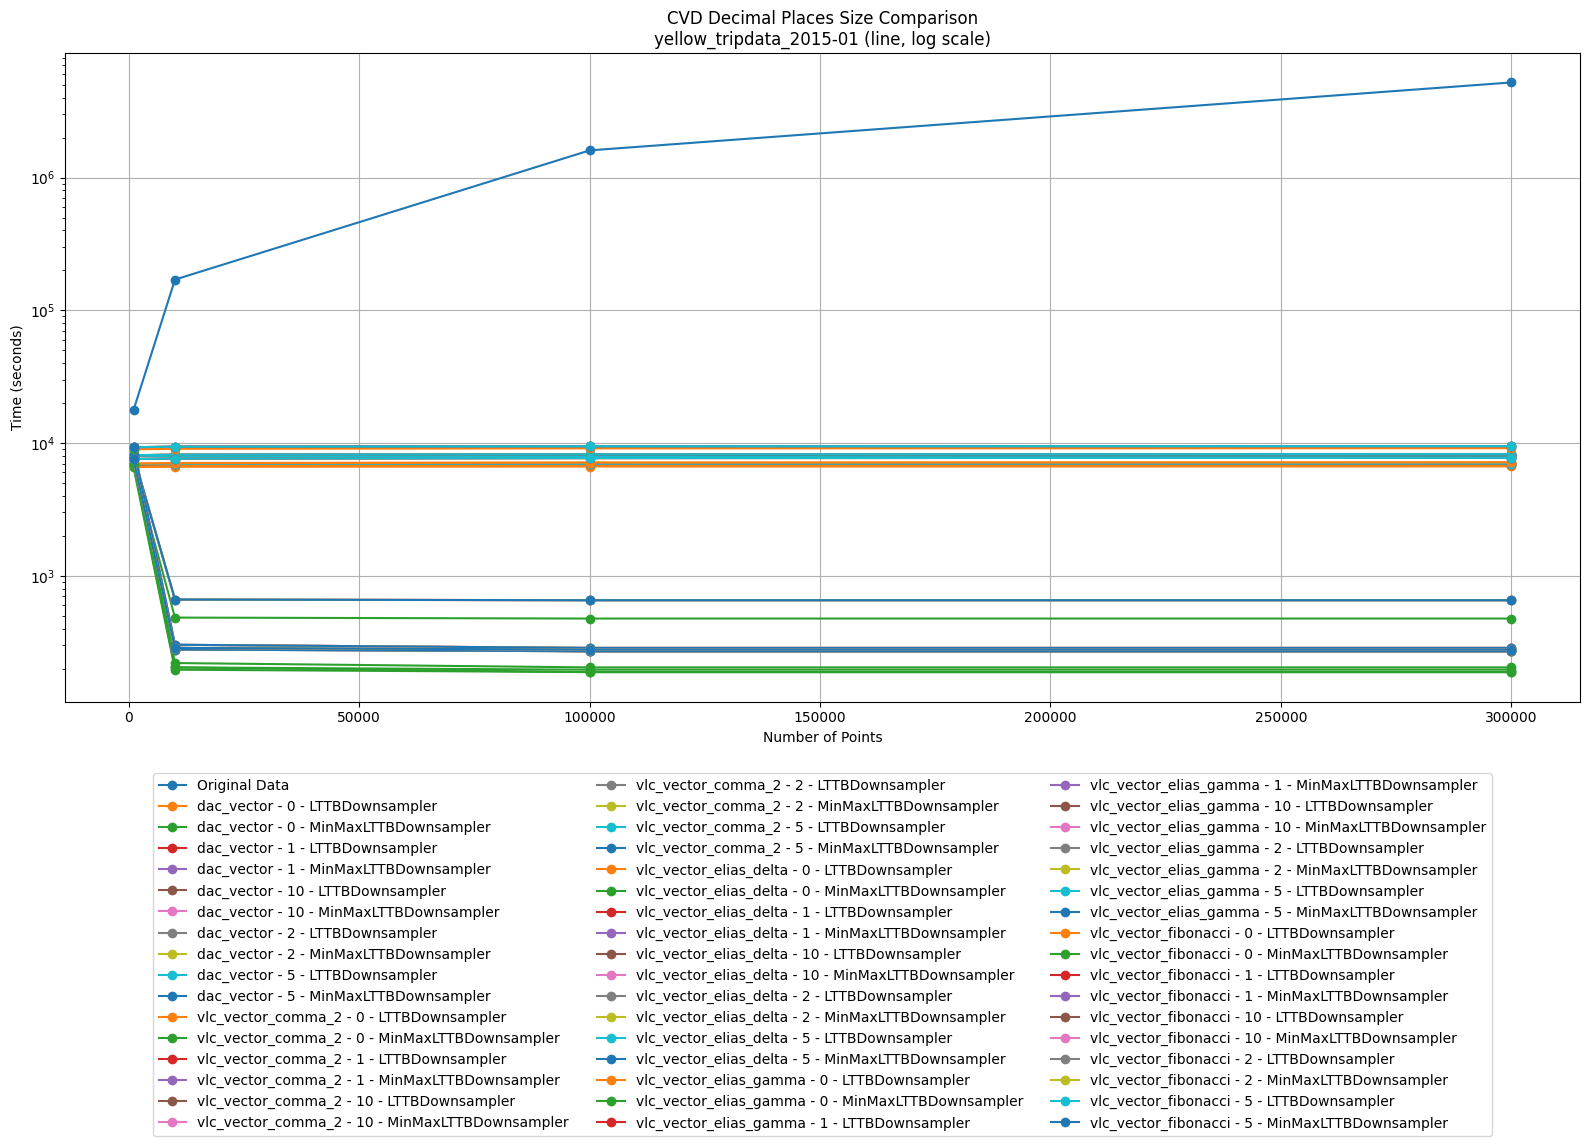
\includegraphics[width=1\textwidth]{anexo/exp/CVD Decimal Places Size Comparison/plots/CVD Decimal Places Size Comparison_yellow_tripdata_2015-01_log_line.png}
        \caption[]{Gráfico de tamaño CVD con diferentes lugares decimales para el input \textbf{yellow\_tripdata\_2015\_01} en escala logarítmica.}
        \label{fig:cvd_decimal_places_size_comparison_plot_log_3}
    \end{figure}
}





% PyGal Plotting Memory Allocation
\DeclareRobustCommand{\PyGalMemoryAllocationOnePlotLine}{
    %insertar imagen
    \begin{figure}[H]
        \centering
        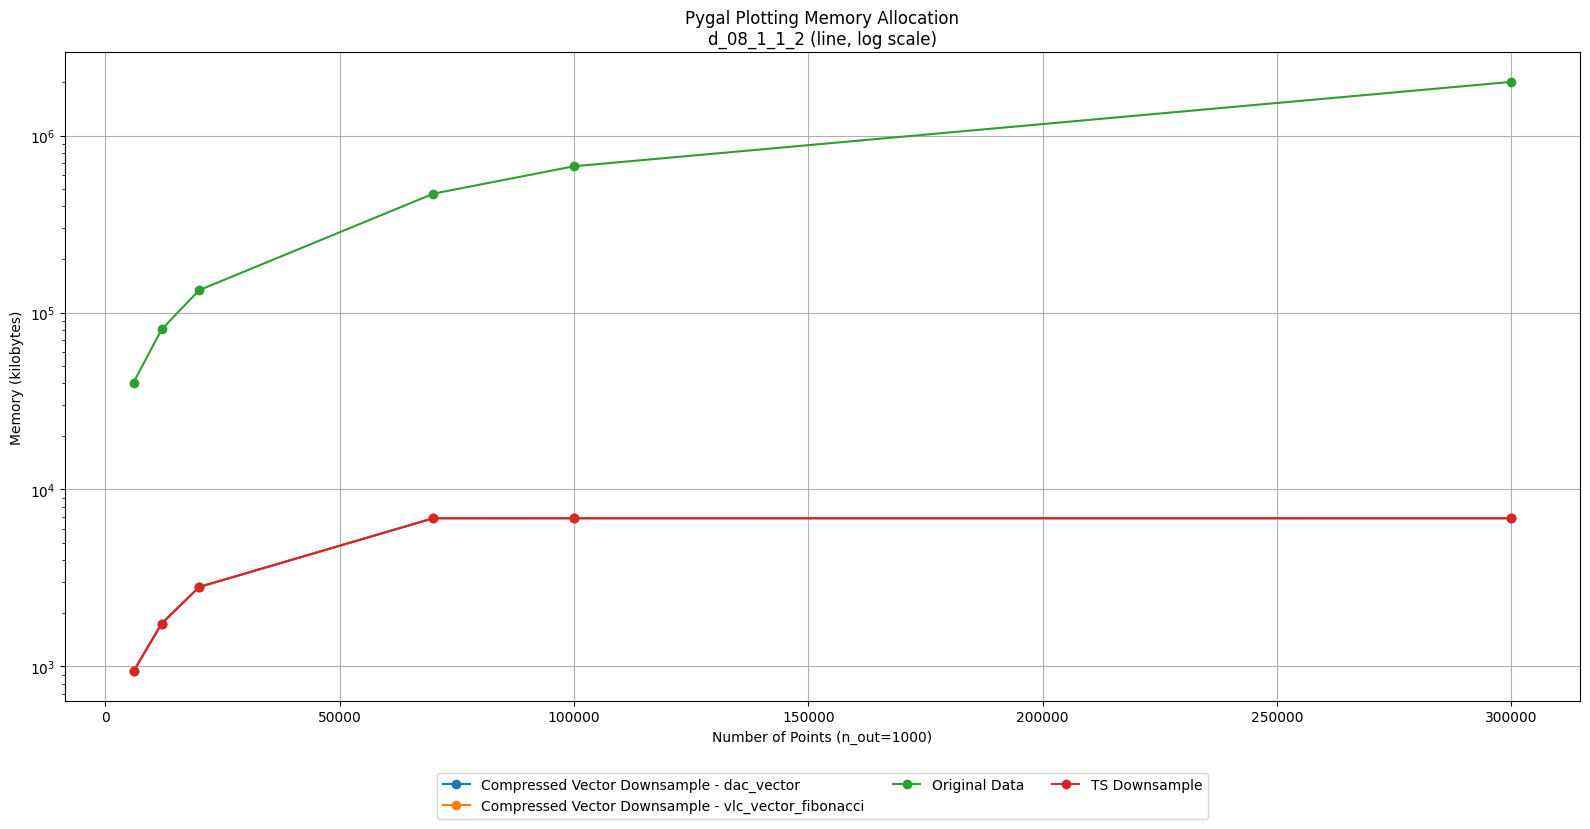
\includegraphics[width=1\textwidth]{anexo/exp/Pygal Plotting Memory Allocation/plots/Pygal Plotting Memory Allocation_d_08_1_1_2_log_line.png}
        \caption[]{Gráfico de memoria asignada por PyGal para el input \textbf{d\_08\_1\_1\_2}.}
        \label{fig:pygal_memory_allocation_plot_line_1}
    \end{figure}
}

\DeclareRobustCommand{\PyGalMemoryAllocationOnePlotBar}{
    %insertar imagen
    \begin{figure}[H]
        \centering
        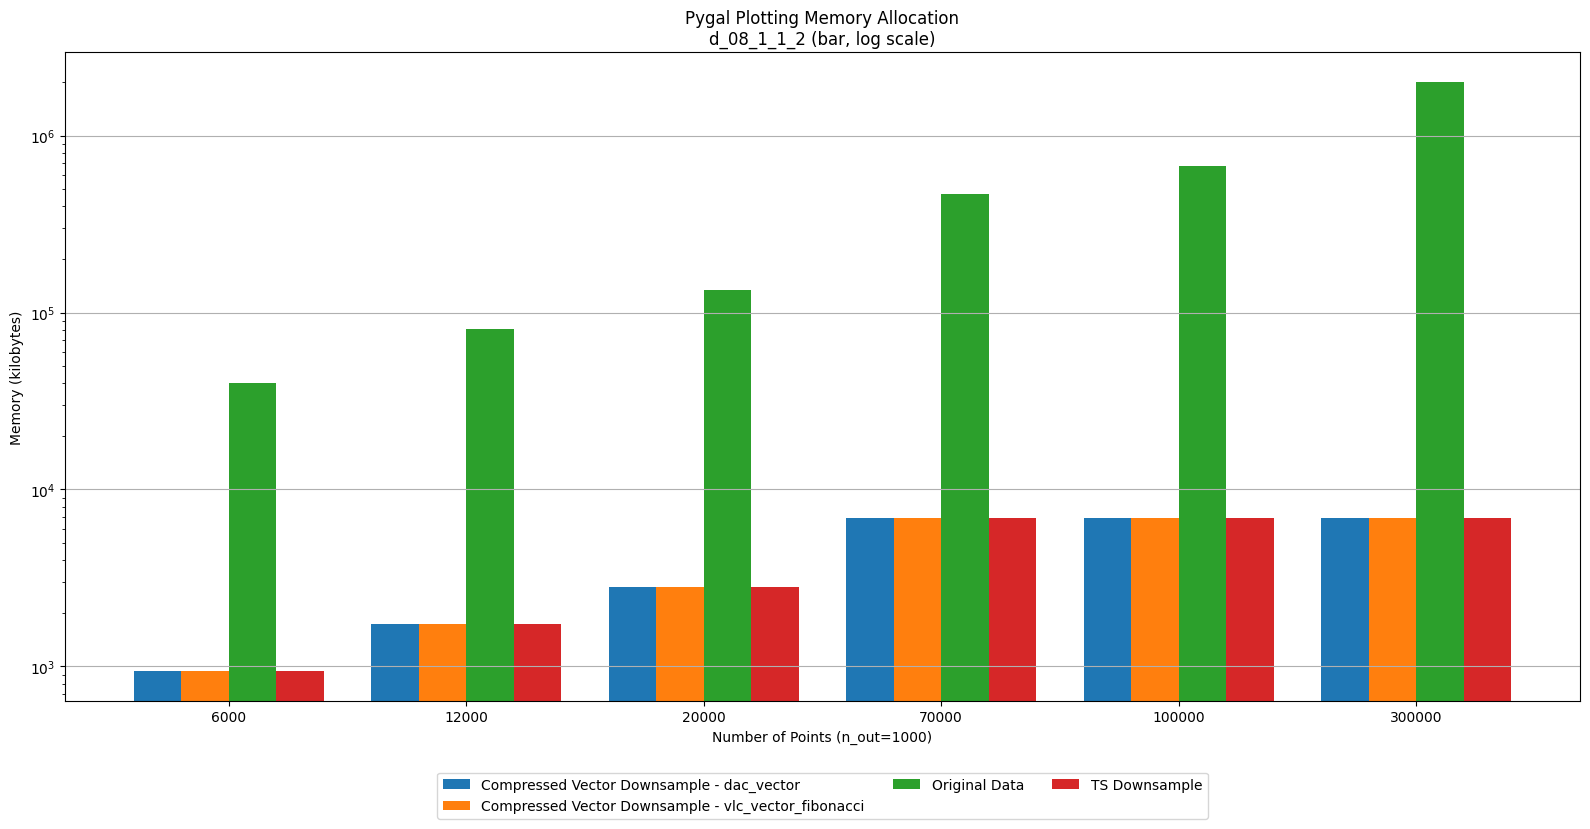
\includegraphics[width=1\textwidth]{anexo/exp/Pygal Plotting Memory Allocation/bar_plots/Pygal Plotting Memory Allocation_d_08_1_1_2_log_bar.png}
        \caption[]{Gráfico de memoria asignada por PyGal para el input \textbf{d\_08\_1\_1\_2}.}
        \label{fig:pygal_memory_allocation_plot_bar_1}
    \end{figure}
\begin{table}[H]
\centering
\resizebox{\textwidth}{!}{%
\begin{tabular}{|l|c|c|c|c|c|c|}
\hline\multicolumn{1}{|c|}{Option} & \multicolumn{6}{c|}{\textbf{Number of data points}} \\
\cline{2-7}
 & \textbf{6000} & \textbf{12000} & \textbf{20000} & \textbf{70000} & \textbf{100000} & \textbf{300000} \\
\hline
Compressed Vector Downsample - dac\_vector & 9.38e+02 [kb] & 1.75e+03 [kb] & 2.81e+03 [kb] & 6.88e+03 [kb] & 6.88e+03 [kb] & 6.88e+03 [kb] \\
Compressed Vector Downsample - vlc\_vector\_fibonacci & 9.38e+02 [kb] & 1.75e+03 [kb] & 2.81e+03 [kb] & 6.88e+03 [kb] & 6.88e+03 [kb] & 6.88e+03 [kb] \\
Original Data & 4.02e+04 [kb] & 8.03e+04 [kb] & 1.34e+05 [kb] & 4.70e+05 [kb] & 6.71e+05 [kb] & 2.01e+06 [kb] \\
TS Downsample & 9.37e+02 [kb] & 1.75e+03 [kb] & 2.81e+03 [kb] & 6.88e+03 [kb] & 6.88e+03 [kb] & 6.88e+03 [kb] \\
\hline
\end{tabular}
}
\label{tab:pygal plotting memory allocation-d-08-1-1-2}
\end{table}
   \begin{table}[H]
\centering
\caption{\textit{d\_08\_1\_1\_2} – Memoria por elemento}
\label{tab:d\_08\_1\_1\_2_mem_por_elemento_sin_original}
\begin{tabular}{rrrr}
\toprule
 & CVD - dac\_vector & CVD - vlc\_vector\_fibonacci & TS Downsample \\
n\_size &  &  &  \\
\midrule
6000 & 0.94 & 0.94 & 0.94 \\
12000 & 1.75 & 1.75 & 1.75 \\
20000 & 2.81 & 2.81 & 2.81 \\
70000 & 6.88 & 6.88 & 6.88 \\
100000 & 6.88 & 6.88 & 6.88 \\
300000 & 6.88 & 6.88 & 6.88 \\
\bottomrule
\end{tabular}

\end{table}
}

\DeclareRobustCommand{\PyGalMemoryAllocationTwoPlotLine}{
    %insertar imagen
    \begin{figure}[H]
        \centering
        \includegraphics[width=1\textwidth]{anexo/exp/PyGal Plotting Memory Allocation/plots/PyGal Plotting Memory Allocation_d_08_1_1_10_linear_line.png}
        \caption[]{Gráfico de memoria asignada por PyGal para el input \textbf{d\_08\_1\_1\_10}.}
        \label{fig:pygal_memory_allocation_plot_line_2}
    \end{figure}
}

\DeclareRobustCommand{\PyGalMemoryAllocationTwoPlotBar}{
    %insertar imagen
    \begin{figure}[H]
        \centering
        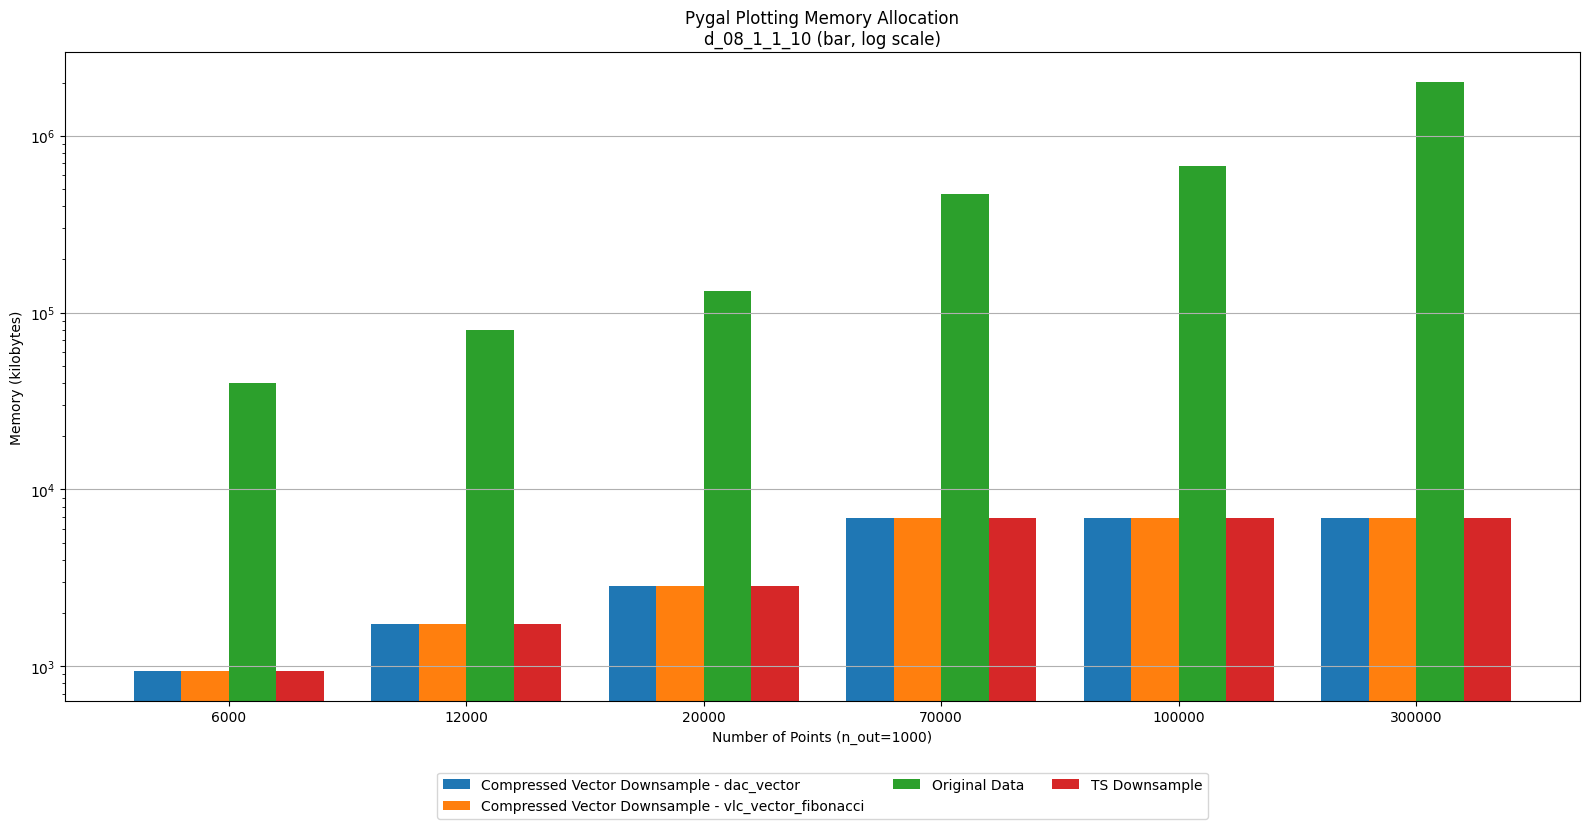
\includegraphics[width=1\textwidth]{anexo/exp/Pygal Plotting Memory Allocation/bar_plots/Pygal Plotting Memory Allocation_d_08_1_1_10_log_bar.png}
        \caption[]{Gráfico de memoria asignada por PyGal para el input \textbf{d\_08\_1\_1\_10}.}
        \label{fig:pygal_memory_allocation_plot_bar_2}
    \end{figure}

\begin{table}[H]
\centering
\resizebox{\textwidth}{!}{%
\begin{tabular}{|l|c|c|c|c|c|c|}
\hline\multicolumn{1}{|c|}{Option} & \multicolumn{6}{c|}{\textbf{Number of data points}} \\
\cline{2-7}
 & \textbf{6000} & \textbf{12000} & \textbf{20000} & \textbf{70000} & \textbf{100000} & \textbf{300000} \\
\hline
Compressed Vector Downsample - dac_vector & 9.36e+02 [kb] & 1.74e+03 [kb] & 2.83e+03 [kb] & 6.88e+03 [kb] & 6.88e+03 [kb] & 6.89e+03 [kb] \\
Compressed Vector Downsample - vlc_vector_fibonacci & 9.36e+02 [kb] & 1.75e+03 [kb] & 2.83e+03 [kb] & 6.88e+03 [kb] & 6.88e+03 [kb] & 6.89e+03 [kb] \\
Original Data & 4.01e+04 [kb] & 8.01e+04 [kb] & 1.33e+05 [kb] & 4.70e+05 [kb] & 6.71e+05 [kb] & 2.02e+06 [kb] \\
TS Downsample & 9.36e+02 [kb] & 1.74e+03 [kb] & 2.83e+03 [kb] & 6.88e+03 [kb] & 6.88e+03 [kb] & 6.90e+03 [kb] \\
\hline
\end{tabular}
}
\label{tab:pygal plotting memory allocation-d-08-1-1-10}
\end{table}
\begin{table}[H]
\centering
\caption{\textit{d\_08\_1\_1\_10} – Memoria por elemento}
\label{tab:d\_08\_1\_1\_10_mem_por_elemento_sin_original}
\begin{tabular}{rrrr}
\toprule
 & CVD - dac\_vector & CVD - vlc\_vector\_fibonacci & TS Downsample \\
n\_size &  &  &  \\
\midrule
6000 & 0.94 & 0.94 & 0.94 \\
12000 & 1.74 & 1.75 & 1.74 \\
20000 & 2.83 & 2.83 & 2.83 \\
70000 & 6.88 & 6.88 & 6.88 \\
100000 & 6.88 & 6.88 & 6.88 \\
300000 & 6.89 & 6.89 & 6.90 \\
\bottomrule
\end{tabular}

\end{table}
}

\DeclareRobustCommand{\PyGalMemoryAllocationThreePlotLine}{
    %insertar imagen
    \begin{figure}[H]
        \centering
        \includegraphics[width=1\textwidth]{anexo/exp/PyGal Plotting Memory Allocation/plots/PyGal Plotting Memory Allocation_yellow_tripdata_2015-01_linear_line.png}
        \caption[]{Gráfico de memoria asignada por PyGal para el input \textbf{yellow\_tripdata\_2015\_01}.}
        \label{fig:pygal_memory_allocation_plot_line_3}
    \end{figure}
}

\DeclareRobustCommand{\PyGalMemoryAllocationThreePlotBar}{
    %insertar imagen
    \begin{figure}[H]
        \centering
        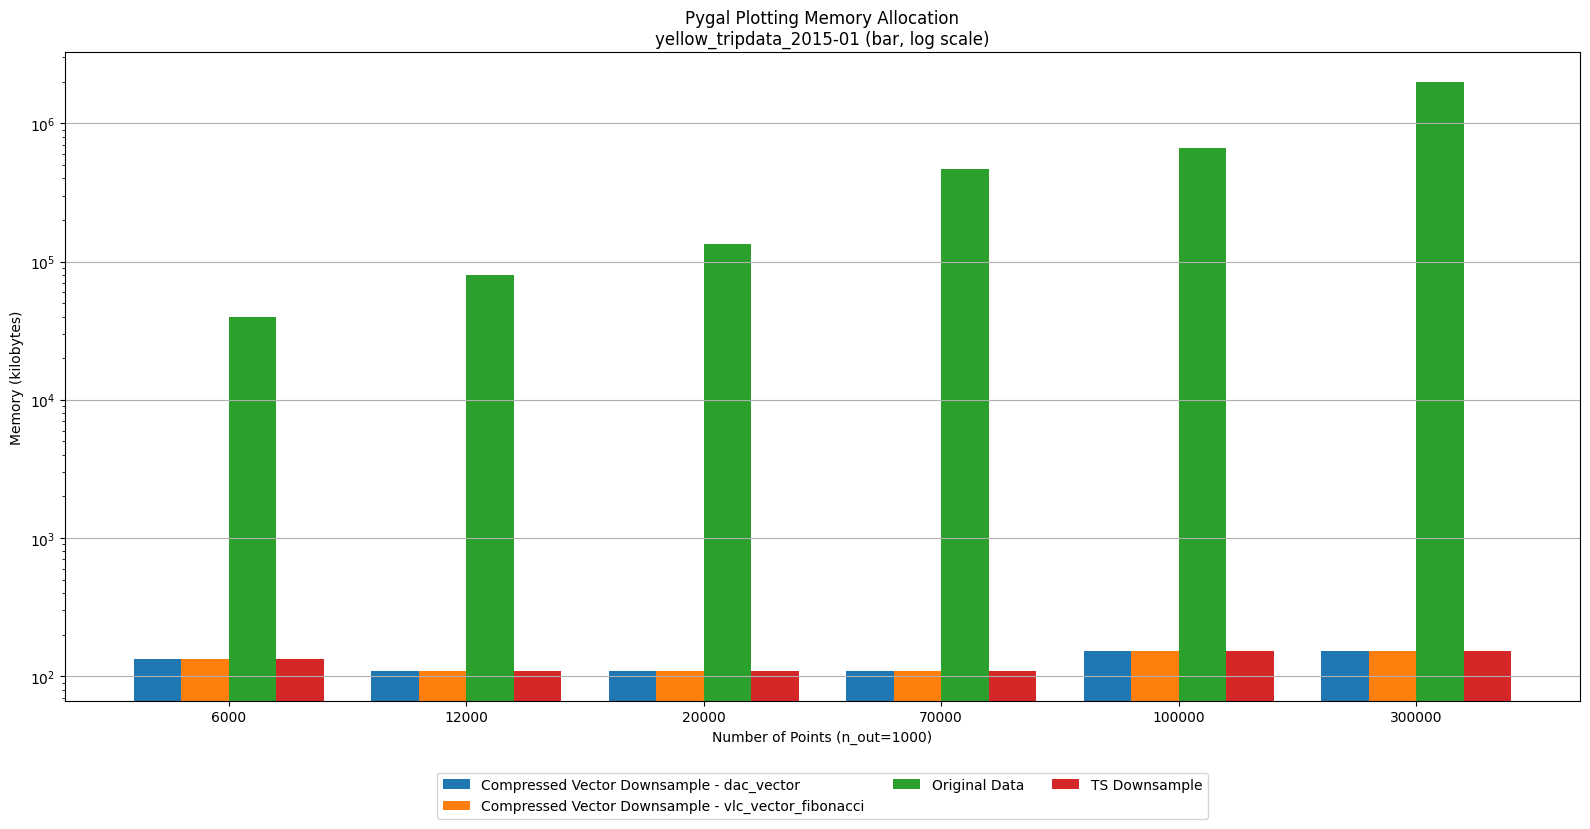
\includegraphics[width=1\textwidth]{anexo/exp/Pygal Plotting Memory Allocation/bar_plots/Pygal Plotting Memory Allocation_yellow_tripdata_2015-01_log_bar.png}
        \caption[]{Gráfico de memoria asignada por PyGal para el input \textbf{yellow\_tripdata\_2015\_01}.}
        \label{fig:pygal_memory_allocation_plot_bar_3}
    \end{figure}
\begin{table}[H]
\centering
\resizebox{\textwidth}{!}{%
\begin{tabular}{|l|c|c|c|c|c|c|}
\hline\multicolumn{1}{|c|}{Option} & \multicolumn{6}{c|}{\textbf{Number of data points}} \\
\cline{2-7}
 & \textbf{6000} & \textbf{12000} & \textbf{20000} & \textbf{70000} & \textbf{100000} & \textbf{300000} \\
\hline
Compressed Vector Downsample - dac_vector & 1.33e+02 [kb] & 1.09e+02 [kb] & 1.09e+02 [kb] & 1.09e+02 [kb] & 1.53e+02 [kb] & 1.52e+02 [kb] \\
Compressed Vector Downsample - vlc_vector_fibonacci & 1.33e+02 [kb] & 1.09e+02 [kb] & 1.10e+02 [kb] & 1.09e+02 [kb] & 1.53e+02 [kb] & 1.53e+02 [kb] \\
Original Data & 4.00e+04 [kb] & 7.99e+04 [kb] & 1.33e+05 [kb] & 4.65e+05 [kb] & 6.64e+05 [kb] & 2.00e+06 [kb] \\
TS Downsample & 1.32e+02 [kb] & 1.09e+02 [kb] & 1.09e+02 [kb] & 1.08e+02 [kb] & 1.53e+02 [kb] & 1.53e+02 [kb] \\
\hline
\end{tabular}
}
\label{tab:pygal plotting memory allocation-yellow-tripdata-2015-01}
\end{table}
\begin{table}[H]
\centering
\caption{\textit{yellow\_tripdata\_2015-01} – Memoria por elemento}
\label{tab:yellow\_tripdata\_2015-01_mem_por_elemento_sin_original}
\begin{tabular}{rrrr}
\toprule
 & CVD - dac\_vector & CVD - vlc\_vector\_fibonacci & TS Downsample \\
n\_size &  &  &  \\
\midrule
6000 & 0.13 & 0.13 & 0.13 \\
12000 & 0.11 & 0.11 & 0.11 \\
20000 & 0.11 & 0.11 & 0.11 \\
70000 & 0.11 & 0.11 & 0.11 \\
100000 & 0.15 & 0.15 & 0.15 \\
300000 & 0.15 & 0.15 & 0.15 \\
\bottomrule
\end{tabular}

\end{table}
}

% PyGal Plot Time
\DeclareRobustCommand{\PyGalPlotTimeOnePlotLine}{
    %insertar imagen
    \begin{figure}[H]
        \centering
        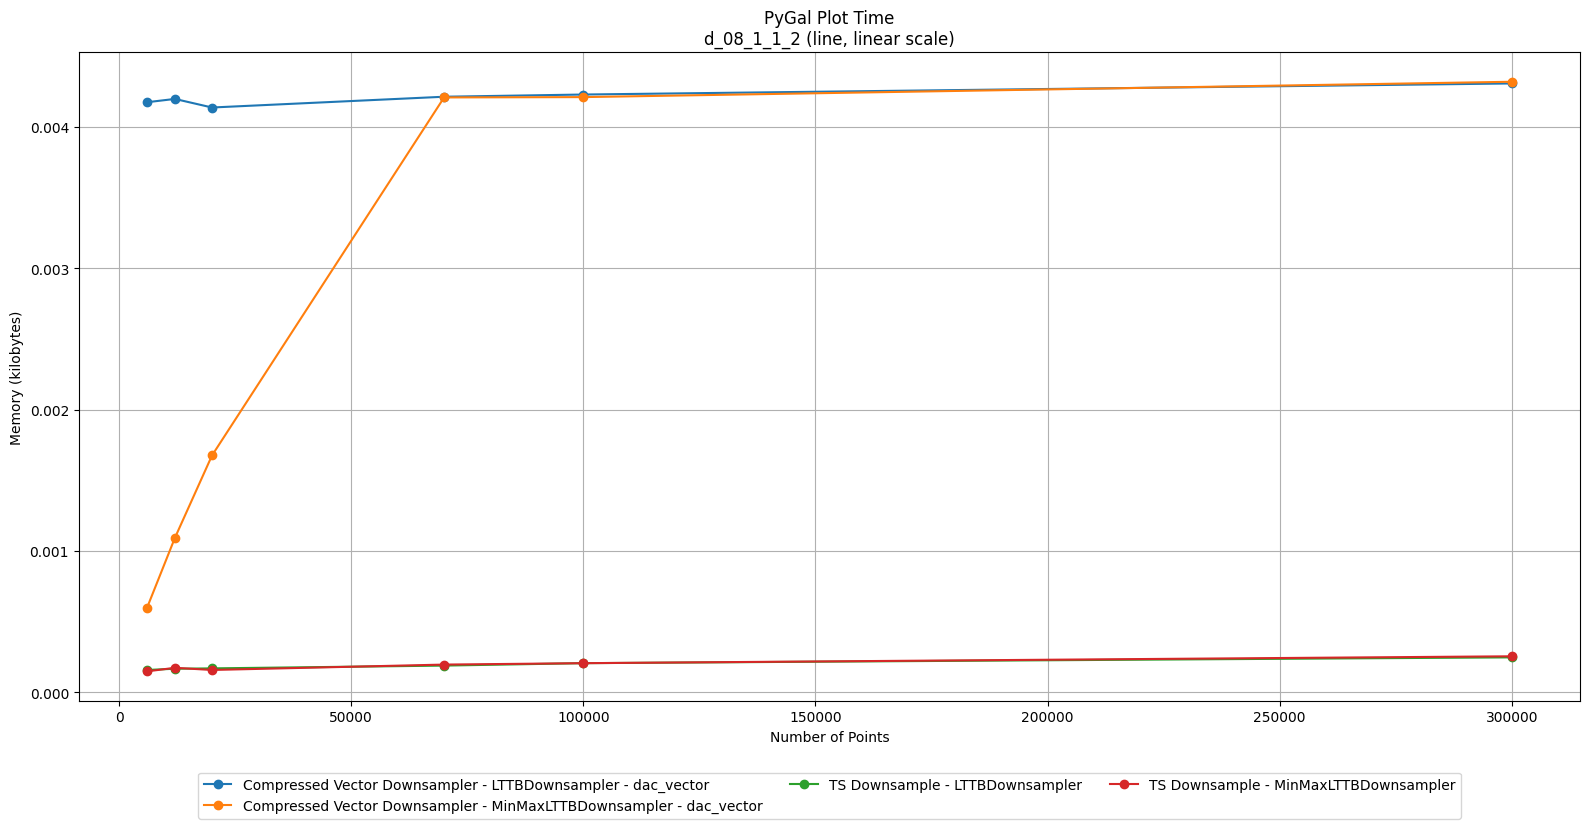
\includegraphics[width=1\textwidth]{anexo/exp/PyGal Plot Time/plots/PyGal Plot Time_d_08_1_1_2_linear_line.png}
        \caption[]{Gráfico de tiempo de renderización PyGal para el input \textbf{d\_08\_1\_1\_2}.}
        \label{fig:pygal_plot_time_plot_line_1}
    \end{figure}
    \begin{figure}[H]
        \centering
        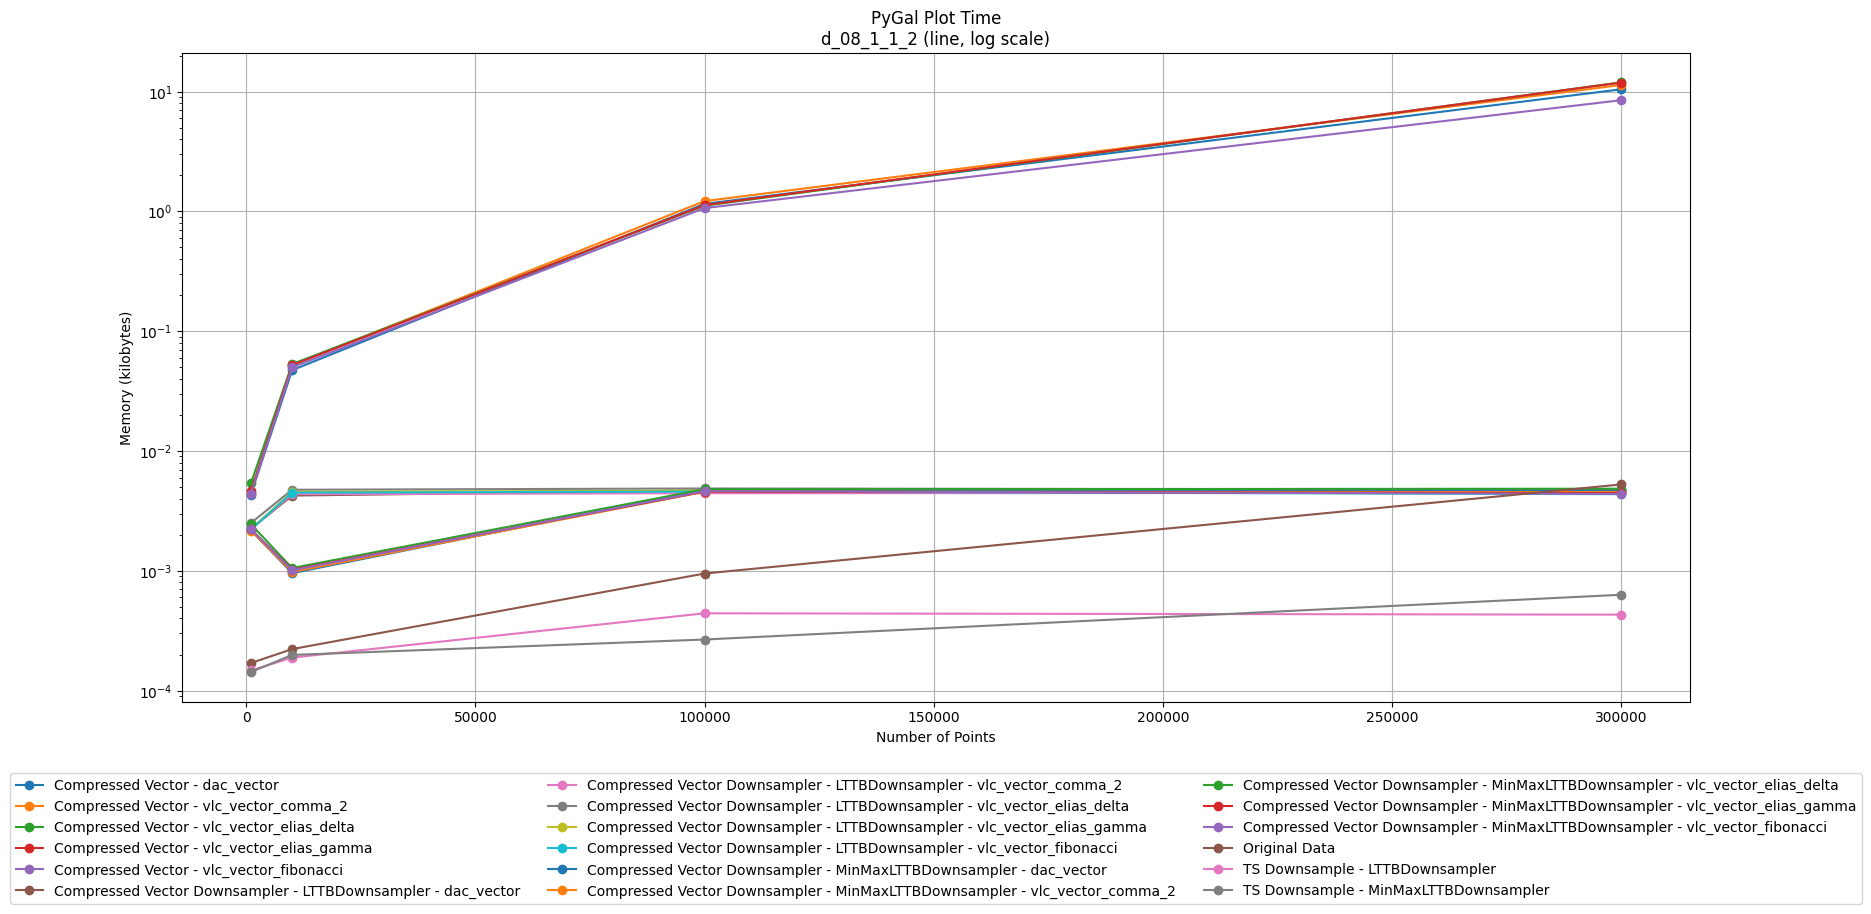
\includegraphics[width=1\textwidth]{anexo/exp/PyGal Plot Time/plots/PyGal Plot Time_d_08_1_1_2_log_line.png}
        \caption[]{Gráfico de tiempo de renderización PyGal para el input \textbf{d\_08\_1\_1\_2} en escala logarítmica.}
        \label{fig:pygal_plot_time_plot_line_1_log}
    \end{figure}
}

\DeclareRobustCommand{\PyGalPlotTimeOnePlotBar}{
    %insertar imagen
    \begin{figure}[H]
        \centering
        \includegraphics[width=1\textwidth]{anexo/exp/PyGal Plot Time/bar_plots/PyGal Plot Time_d_08_1_1_2_linear_bar.png}
        \caption[]{Gráfico de tiempo de renderización PyGal para el input \textbf{d\_08\_1\_1\_2}.}
        \label{fig:pygal_plot_time_plot_bar_1}
    \end{figure}
}

\DeclareRobustCommand{\PyGalPlotTimeTwoPlotLine}{
    %insertar imagen
    \begin{figure}[H]
        \centering
        \includegraphics[width=1\textwidth]{anexo/exp/PyGal Plot Time/plots/PyGal Plot Time_d_08_1_1_10_linear_line.png}
        \caption[]{Gráfico de tiempo de renderización PyGal para el input \textbf{d\_08\_1\_1\_10}.}
        \label{fig:pygal_plot_time_plot_line_2}
    \end{figure}
    \begin{figure}[H]
        \centering
        \includegraphics[width=1\textwidth]{anexo/exp/PyGal Plot Time/plots/PyGal Plot Time_d_08_1_1_10_log_line.png}
        \caption[]{Gráfico de tiempo de renderización PyGal para el input \textbf{d\_08\_1\_1\_10} en escala logarítmica.}
        \label{fig:pygal_plot_time_plot_line_2_log}
    \end{figure}
}

\DeclareRobustCommand{\PyGalPlotTimeTwoPlotBar}{
    %insertar imagen
    \begin{figure}[H]
        \centering
        \includegraphics[width=1\textwidth]{anexo/exp/PyGal Plot Time/bar_plots/PyGal Plot Time_d_08_1_1_10_linear_bar.png}
        \caption[]{Gráfico de tiempo de renderización PyGal para el input \textbf{d\_08\_1\_1\_10}.}
        \label{fig:pygal_plot_time_plot_bar_2}
    \end{figure}
}

\DeclareRobustCommand{\PyGalPlotTimeThreePlotLine}{
    %insertar imagen
    \begin{figure}[H]
        \centering
        \includegraphics[width=1\textwidth]{anexo/exp/PyGal Plot Time/plots/PyGal Plot Time_yellow_tripdata_2015-01_linear_line.png}
        \caption[]{Gráfico de tiempo de renderización PyGal para el input \textbf{yellow\_tripdata\_2015\_01}.}
        \label{fig:pygal_plot_time_plot_line_3}
    \end{figure}
    \begin{figure}[H]
        \centering
        \includegraphics[width=1\textwidth]{anexo/exp/PyGal Plot Time/plots/PyGal Plot Time_yellow_tripdata_2015-01_log_line.png}
        \caption[]{Gráfico de tiempo de renderización PyGal para el input \textbf{yellow\_tripdata\_2015\_01}.}
        \label{fig:pygal_plot_time_plot_line_3_log}
    \end{figure}
}

\DeclareRobustCommand{\PyGalPlotTimeThreePlotBar}{
    %insertar imagen
    \begin{figure}[H]
        \centering
        \includegraphics[width=1\textwidth]{anexo/exp/PyGal Plot Time/bar_plots/PyGal Plot Time_yellow_tripdata_2015-01_linear_bar.png}
        \caption[]{Gráfico de tiempo de renderización PyGal para el input \textbf{yellow\_tripdata\_2015\_01}.}
        \label{fig:pygal_plot_time_plot_bar_3}
    \end{figure}
}

\DeclareRobustCommand{\SDSLFourPyAccessTimeComparisonOnePlotBar}{
    \begin{figure}[H]
        \centering
        \includegraphics[width=1\textwidth]{anexo/exp/SDSL4Py Access Time Comparison/bar_plots/SDSL4Py Access Time Comparison_d_08_1_1_2_log_bar.png}
        \caption[]{Gráfico de tiempo de acceso SDSL4Py en escala logarítmica para el input \textbf{d\_08\_1\_1\_2}.}
        \label{fig:sdsl4py_access_time_comparison_plot_log_bar_1}
    \end{figure}
}

\DeclareRobustCommand{\SDSLFourPyAccessTimeComparisonTwoPlotBar}{
    \begin{figure}[H]
        \centering
        \includegraphics[width=1\textwidth]{anexo/exp/SDSL4Py Access Time Comparison/bar_plots/SDSL4Py Access Time Comparison_d_08_1_1_10_log_bar.png}
        \caption[]{Gráfico de tiempo de acceso SDSL4Py en escala logarítmica para el input \textbf{d\_08\_1\_1\_10}.}
        \label{fig:sdsl4py_access_time_comparison_plot_log_bar_2}
    \end{figure}
}

\DeclareRobustCommand{\SDSLFourPyAccessTimeComparisonThreePlotBar}{
    \begin{figure}[H]
        \centering
        \includegraphics[width=1\textwidth]{anexo/exp/SDSL4Py Access Time Comparison/bar_plots/SDSL4Py Access Time Comparison_yellow_tripdata_2015-01_log_bar.png}
        \caption[]{Gráfico de tiempo de acceso SDSL4Py en escala logarítmica para el input \textbf{yellow\_tripdata\_2015\_01}.}
        \label{fig:sdsl4py_access_time_comparison_plot_log_bar_3}
    \end{figure}
}

\DeclareRobustCommand{\SDSLFourPyCompressionSpaceComparisonOnePlotBar}{
    \begin{figure}[H]
        \centering
        \includegraphics[width=1\textwidth]{anexo/exp/SDSL4Py Compression Space Comparison/bar_plots/SDSL4Py Compression Space Comparison_d_08_1_1_2_log_bar.png}
        \caption[]{Gráfico de espacio de compresión SDSL4Py en escala logarítmica para el input \textbf{d\_08\_1\_1\_2}.}
        \label{fig:sdsl4py_compression_space_comparison_plot_log_bar_1}
    \end{figure}
}

\DeclareRobustCommand{\SDSLFourPyCompressionSpaceComparisonTwoPlotBar}{
    \begin{figure}[H]
        \centering
        \includegraphics[width=1\textwidth]{anexo/exp/SDSL4Py Compression Space Comparison/bar_plots/SDSL4Py Compression Space Comparison_d_08_1_1_10_log_bar.png}
        \caption[]{Gráfico de espacio de compresión SDSL4Py en escala logarítmica para el input \textbf{d\_08\_1\_1\_10}.}
        \label{fig:sdsl4py_compression_space_comparison_plot_log_bar_2}
    \end{figure}
}

\DeclareRobustCommand{\SDSLFourPyCompressionSpaceComparisonThreePlotBar}{
    \begin{figure}[H]
        \centering
        \includegraphics[width=1\textwidth]{anexo/exp/SDSL4Py Compression Space Comparison/bar_plots/SDSL4Py Compression Space Comparison_yellow_tripdata_2015-01_log_bar.png}
        \caption[]{Gráfico de espacio de compresión SDSL4Py en escala logarítmica para el input \textbf{yellow\_tripdata\_2015\_01}.}
        \label{fig:sdsl4py_compression_space_comparison_plot_log_bar_3}
    \end{figure}
}
\DeclareRobustCommand{\SDSLFourPyCompressionTimeComparisonOnePlotBar}{
    \begin{figure}[H]
        \centering
        \includegraphics[width=1\textwidth]{anexo/exp/SDSL4Py Compression Time Comparison/bar_plots/SDSL4Py Compression Time Comparison_d_08_1_1_2_log_bar.png}
        \caption[]{Gráfico de tiempo de compresión SDSL4Py en escala logarítmica para el input \textbf{d\_08\_1\_1\_2}.}
        \label{fig:sdsl4py_compression_time_comparison_plot_log_bar_1}
    \end{figure}
}

\DeclareRobustCommand{\SDSLFourPyCompressionTimeComparisonTwoPlotBar}{
    \begin{figure}[H]
        \centering
        \includegraphics[width=1\textwidth]{anexo/exp/SDSL4Py Compression Time Comparison/bar_plots/SDSL4Py Compression Time Comparison_d_08_1_1_10_log_bar.png}
        \caption[]{Gráfico de tiempo de compresión SDSL4Py en escala logarítmica para el input \textbf{d\_08\_1\_1\_10}.}
        \label{fig:sdsl4py_compression_time_comparison_plot_log_bar_2}
    \end{figure}
}

\DeclareRobustCommand{\SDSLFourPyCompressionTimeComparisonThreePlotBar}{
    \begin{figure}[H]
        \centering
        \includegraphics[width=1\textwidth]{anexo/exp/SDSL4Py Compression Time Comparison/bar_plots/SDSL4Py Compression Time Comparison_yellow_tripdata_2015-01_log_bar.png}
        \caption[]{Gráfico de tiempo de compresión SDSL4Py en escala logarítmica para el input \textbf{yellow\_tripdata\_2015\_01}.}
        \label{fig:sdsl4py_compression_time_comparison_plot_log_bar_3}
    \end{figure}
}


% Vega-Altair Plot Time Comparison
\DeclareRobustCommand{\VegaAltairPlotTimeComparisonOnePlotLine}{
    %insertar imagen
    \begin{figure}[H]
        \centering
        \includegraphics[width=1\textwidth]{anexo/exp/Vega-Altair Plot Time Comparison/plots/Vega-Altair Plot Time Comparison_d_08_1_1_2_linear_line.png}
        \caption[]{Gráfico de tiempo de renderización Vega-Altair para el input \textbf{d\_08\_1\_1\_2}.}
        \label{fig:vega_altair_plot_time_comparison_plot_line_1}
    \end{figure}
    \begin{figure}[H]
        \centering
        \includegraphics[width=1\textwidth]{anexo/exp/Vega-Altair Plot Time Comparison/plots/Vega-Altair Plot Time Comparison_d_08_1_1_2_log_line.png}
        \caption[]{Gráfico de tiempo de renderización Vega-Altair para el input \textbf{d\_08\_1\_1\_2} en escala logarítmica.}
        \label{fig:vega_altair_plot_time_comparison_plot_line_1}
    \end{figure}
}

\DeclareRobustCommand{\VegaAltairPlotTimeComparisonOnePlotBar}{
    %insertar imagen
    \begin{figure}[H]
        \centering
        \includegraphics[width=1\textwidth]{anexo/exp/Vega-Altair Plot Time Comparison/bar_plots/Vega-Altair Plot Time Comparison_d_08_1_1_2_linear_bar.png}
        \caption[]{Gráfico de tiempo de renderización Vega-Altair para el input \textbf{d\_08\_1\_1\_2}.}
        \label{fig:vega_altair_plot_time_comparison_plot_bar_1}
    \end{figure}
}

\DeclareRobustCommand{\VegaAltairPlotTimeComparisonTwoPlotLine}{
    %insertar imagen
    \begin{figure}[H]
        \centering
        \includegraphics[width=1\textwidth]{anexo/exp/Vega-Altair Plot Time Comparison/plots/Vega-Altair Plot Time Comparison_d_08_1_1_10_linear_line.png}
        \caption[]{Gráfico de tiempo de renderización Vega-Altair para el input \textbf{d\_08\_1\_1\_10}.}
        \label{fig:vega_altair_plot_time_comparison_plot_line_2}
    \end{figure}
}

\DeclareRobustCommand{\VegaAltairPlotTimeComparisonTwoPlotBar}{
    %insertar imagen
    \begin{figure}[H]
        \centering
        \includegraphics[width=1\textwidth]{anexo/exp/Vega-Altair Plot Time Comparison/bar_plots/Vega-Altair Plot Time Comparison_d_08_1_1_10_linear_bar.png}
        \caption[]{Gráfico de tiempo de renderización Vega-Altair para el input \textbf{d\_08\_1\_1\_10}.}
        \label{fig:vega_altair_plot_time_comparison_plot_bar_2}
    \end{figure}
}

\DeclareRobustCommand{\VegaAltairPlotTimeComparisonThreePlotLine}{
    %insertar imagen
    \begin{figure}[H]
        \centering
        \includegraphics[width=1\textwidth]{anexo/exp/Vega-Altair Plot Time Comparison/plots/Vega-Altair Plot Time Comparison_yellow_tripdata_2015-01_linear_line.png}
        \caption[]{Gráfico de tiempo de renderización Vega-Altair para el input \textbf{yellow\_tripdata\_2015\_01}.}
        \label{fig:vega_altair_plot_time_comparison_plot_line_3}
    \end{figure}
}

\DeclareRobustCommand{\VegaAltairPlotTimeComparisonThreePlotBar}{
    %insertar imagen
    \begin{figure}[H]
        \centering
        \includegraphics[width=1\textwidth]{anexo/exp/Vega-Altair Plot Time Comparison/bar_plots/Vega-Altair Plot Time Comparison_yellow_tripdata_2015-01_linear_bar.png}
        \caption[]{Gráfico de tiempo de renderización Vega-Altair para el input \textbf{yellow\_tripdata\_2015\_01}.}
        \label{fig:vega_altair_plot_time_comparison_plot_bar_3}
    \end{figure}
}

% Vega-Altair Plotting + Building Comparison
\DeclareRobustCommand{\VegaAltairPlottingBuildingComparisonOnePlotLine}{
    %insertar imagen
    \begin{figure}[H]
        \centering
        \includegraphics[width=1\textwidth]{anexo/exp/Vega-Altair Plotting + Building Comparison/plots/Vega-Altair Plotting + Building Comparison_d_08_1_1_2_linear_line.png}
        \caption[]{Gráfico de tiempo de renderización y construcción Vega-Altair para el input \textbf{d\_08\_1\_1\_2}.}
        \label{fig:vega_altair_plotting_building_comparison_plot_line_1}
    \end{figure}
}

\DeclareRobustCommand{\VegaAltairPlottingBuildingComparisonOnePlotBar}{
    %insertar imagen
    \begin{figure}[H]
        \centering
        \includegraphics[width=1\textwidth]{anexo/exp/Vega-Altair Plotting + Building Comparison/bar_plots/Vega-Altair Plotting + Building Comparison_d_08_1_1_2_linear_bar.png}
        \caption[]{Gráfico de tiempo de renderización y construcción Vega-Altair para el input \textbf{d\_08\_1\_1\_2}.}
        \label{fig:vega_altair_plotting_building_comparison_plot_bar_1}
    \end{figure}
}

\DeclareRobustCommand{\VegaAltairPlottingBuildingComparisonTwoPlotLine}{
    %insertar imagen
    \begin{figure}[H]
        \centering
        \includegraphics[width=1\textwidth]{anexo/exp/Vega-Altair Plotting + Building Comparison/plots/Vega-Altair Plotting + Building Comparison_d_08_1_1_10_linear_line.png}
        \caption[]{Gráfico de tiempo de renderización y construcción Vega-Altair para el input \textbf{d\_08\_1\_1\_10}.}
        \label{fig:vega_altair_plotting_building_comparison_plot_line_2}
    \end{figure}
}

\DeclareRobustCommand{\VegaAltairPlottingBuildingComparisonTwoPlotBar}{
    %insertar imagen
    \begin{figure}[H]
        \centering
        \includegraphics[width=1\textwidth]{anexo/exp/Vega-Altair Plotting + Building Comparison/bar_plots/Vega-Altair Plotting + Building Comparison_d_08_1_1_10_linear_bar.png}
        \caption[]{Gráfico de tiempo de renderización y construcción Vega-Altair para el input \textbf{d\_08\_1\_1\_10}.}
        \label{fig:vega_altair_plotting_building_comparison_plot_bar_2}
    \end{figure}
}

\DeclareRobustCommand{\VegaAltairPlottingBuildingComparisonThreePlotLine}{
    %insertar imagen
    \begin{figure}[H]
        \centering
        \includegraphics[width=1\textwidth]{anexo/exp/Vega-Altair Plotting + Building Comparison/plots/Vega-Altair Plotting + Building Comparison_yellow_tripdata_2015-01_linear_line.png}
        \caption[]{Gráfico de tiempo de renderización y construcción Vega-Altair para el input \textbf{yellow\_tripdata\_2015\_01}.}
        \label{fig:vega_altair_plotting_building_comparison_plot_line_3}
    \end{figure}
}

\DeclareRobustCommand{\VegaAltairPlottingBuildingComparisonThreePlotBar}{
    %insertar imagen
    \begin{figure}[H]
        \centering
        \includegraphics[width=1\textwidth]{anexo/exp/Vega-Altair Plotting + Building Comparison/bar_plots/Vega-Altair Plotting + Building Comparison_yellow_tripdata_2015-01_linear_bar.png}
        \caption[]{Gráfico de tiempo de renderización y construcción Vega-Altair para el input \textbf{yellow\_tripdata\_2015\_01}.}
        \label{fig:vega_altair_plotting_building_comparison_plot_bar_3}
    \end{figure}
}

% VEGA ALTAIR MEMORY ALLOCATION

\DeclareRobustCommand{\VegaAltairMemoryAllocationOnePlotLine}{
    %insertar imagen
    \begin{figure}[H]
        \centering
        \includegraphics[width=1\textwidth]{anexo/exp/Vega-Altair Plotting Memory Allocation/plots/Vega-Altair Plotting Memory Allocation_d_08_1_1_2_log_line.png}
        \caption[]{Gráfico de tiempo de renderización y construcción Vega-Altair para el input \textbf{d\_08\_1\_1\_2}.}
        \label{fig:vega_altair_plotting_building_comparison_plot_line_1}
    \end{figure}
}

\DeclareRobustCommand{\VegaAltairMemoryAllocationOnePlotBar}{
    %insertar imagen
    \begin{figure}[H]
        \centering
        \includegraphics[width=1\textwidth]{anexo/exp/Vega-Altair Plotting Memory Allocation/bar_plots/Vega-Altair Plotting Memory Allocation_d_08_1_1_2_log_bar.png}
        \caption[]{Gráfico de tiempo de renderización y construcción Vega-Altair para el input \textbf{d\_08\_1\_1\_2}.}
        \label{fig:vega_altair_plotting_building_comparison_plot_bar_1}
    \end{figure}
\begin{table}[H]
\centering
\caption{\textit{d\_08\_1\_1\_2} – Memoria por elemento [KB]}
\label{tab:Vega-Altair Plotting Memory Allocation\_d\_08\_1\_1\_2_mem_por_elemento_sin_original}
\begin{tabular}{rrrr}
\toprule
 & CVD - dac\_vector & CVD - vlc\_vector\_fibonacci & TS Downsample \\
n\_size &  &  &  \\
\midrule
6000 & 0.16 & 0.16 & 0.16 \\
12000 & 0.16 & 0.16 & 0.16 \\
20000 & 0.17 & 0.17 & 0.16 \\
70000 & 0.18 & 0.18 & 0.17 \\
100000 & 0.18 & 0.18 & 0.17 \\
300000 & 0.19 & 0.18 & 0.17 \\
\bottomrule
\end{tabular}

\end{table}
}

\DeclareRobustCommand{\VegaAltairMemoryAllocationTwoPlotLine}{
    %insertar imagen
    \begin{figure}[H]
        \centering
        \includegraphics[width=1\textwidth]{anexo/exp/Vega-Altair Plotting Memory Allocation/plots/Vega-Altair Plotting Memory Allocation_d_08_1_1_10_log_line.png}
        \caption[]{Gráfico de tiempo de renderización y construcción Vega-Altair para el input \textbf{d\_08\_1\_1\_10}.}
        \label{fig:vega_altair_plotting_building_comparison_plot_line_2}
    \end{figure}
}

\DeclareRobustCommand{\VegaAltairMemoryAllocationTwoPlotBar}{
    %insertar imagen
    \begin{figure}[H]
        \centering
        \includegraphics[width=1\textwidth]{anexo/exp/Vega-Altair Plotting Memory Allocation/bar_plots/Vega-Altair Plotting Memory Allocation_d_08_1_1_10_log_bar.png}
        \caption[]{Gráfico de asignación de memoria con la biblioteca Vega-Altair para el input \textbf{d\_08\_1\_1\_10}.}
        \label{fig:vega_altair_plotting_building_comparison_plot_bar_2}
    \end{figure}
\begin{table}[H]
\centering
\caption{\textit{d\_08\_1\_1\_10} – Memoria por elemento [KB]}
\label{tab:Vega-Altair Plotting Memory Allocation\_d\_08\_1\_1\_10_mem_por_elemento_sin_original}
\begin{tabular}{rrrr}
\toprule
 & CVD - dac\_vector & CVD - vlc\_vector\_fibonacci & TS Downsample \\
n\_size &  &  &  \\
\midrule
6000 & 0.16 & 0.16 & 0.16 \\
12000 & 0.16 & 0.16 & 0.16 \\
20000 & 0.17 & 0.17 & 0.16 \\
70000 & 0.18 & 0.18 & 0.17 \\
100000 & 0.18 & 0.18 & 0.17 \\
300000 & 0.18 & 0.20 & 0.17 \\
\bottomrule
\end{tabular}

\end{table}
}

\DeclareRobustCommand{\VegaAltairMemoryAllocationThreePlotLine}{
    %insertar imagen
    \begin{figure}[H]
        \centering
        \includegraphics[width=1\textwidth]{anexo/exp/Vega-Altair Plotting Memory Allocation/plots/Vega-Altair Plotting Memory Allocation_yellow_tripdata_2015-01_log_line.png}
        \caption[]{Gráfico de asignación de memoria con la biblioteca Vega-Altair para el input \textbf{yellow\_tripdata\_2015\_01}.}
        \label{fig:vega_altair_plotting_building_comparison_plot_line_3}
    \end{figure}
}

\DeclareRobustCommand{\VegaAltairMemoryAllocationThreePlotBar}{
    %insertar imagen
    \begin{figure}[H]
        \centering
        \includegraphics[width=1\textwidth]{anexo/exp/Vega-Altair Plotting Memory Allocation/bar_plots/Vega-Altair Plotting Memory Allocation_yellow_tripdata_2015-01_log_bar.png}
        \caption[]{Gráfico de asignación de memoria con la biblioteca Vega-Altair para el input \textbf{yellow\_tripdata\_2015\_01}.}
        \label{fig:vega_altair_plotting_building_comparison_plot_bar_3}
    \end{figure}
\begin{table}[H]
\centering
\caption{\textit{yellow\_tripdata\_2015-01} – Memoria por elemento [KB]}
\label{tab:Vega-Altair Plotting Memory Allocation\_yellow\_tripdata\_2015-01_mem_por_elemento_sin_original}
\begin{tabular}{rrrr}
\toprule
 & CVD - dac\_vector & CVD - vlc\_vector\_fibonacci & TS Downsample \\
n\_size &  &  &  \\
\midrule
6000 & 0.16 & 0.16 & 0.16 \\
12000 & 0.16 & 0.16 & 0.16 \\
20000 & 0.16 & 0.16 & 0.16 \\
70000 & 0.16 & 0.16 & 0.16 \\
100000 & 0.16 & 0.16 & 0.16 \\
300000 & 0.16 & 0.16 & 0.16 \\
\bottomrule
\end{tabular}

\end{table}
}

% All Libraries Memory Allocation

\DeclareRobustCommand{\AllLibrariesMemoryAllocationOneTable}
{
    \vspace{0.5em}
    \input{anexo/exp/All Libraries Memory Allocation/txts/All Libraries Memory Allocation_d_08_1_1_2.txt}
}
\DeclareRobustCommand{\AllLibrariesMemoryAllocationTwoTable}
{
    \vspace{0.5em}
    \input{anexo/exp/All Libraries Memory Allocation/txts/All Libraries Memory Allocation_d_08_1_1_2_10.txt}
}
\DeclareRobustCommand{\AllLibrariesMemoryAllocationThreeTable}
{
    \vspace{0.5em}
    \input{anexo/exp/All Libraries Memory Allocation/txts/All Libraries Memory Allocation_yellow_tripdata_2015-01.txt}
}

% All Libraries Time Comparison
\DeclareRobustCommand{\AllLibrariesTimeComparisonOneTable}
{
    \vspace{0.5em}
    \input{anexo/exp/All Libraries Time Comparison/txts/All Libraries Time Comparison_d_08_1_1_2.txt}
}
\DeclareRobustCommand{\AllLibrariesTimeComparisonTwoTable}
{
    \vspace{0.5em}
    \input{anexo/exp/All Libraries Time Comparison/txts/All Libraries Time Comparison_d_08_1_1_2_10.txt}
}
\DeclareRobustCommand{\AllLibrariesTimeComparisonThreeTable}
{
    \vspace{0.5em}
    \input{anexo/exp/All Libraries Time Comparison/txts/All Libraries Time Comparison_yellow_tripdata_2015-01.txt}
}

% Building Time Comparison
\DeclareRobustCommand{\BuildingTimeComparisonOneTable}
{
    \vspace{0.5em}
    \input{anexo/exp/Building Time Comparison/txts/Building Time Comparison_d_08_1_1_2.txt}
}
\DeclareRobustCommand{\BuildingTimeComparisonTwoTable}
{
    \vspace{0.5em}
    \input{anexo/exp/Building Time Comparison/txts/Building Time Comparison_d_08_1_1_2_10.txt}
}
\DeclareRobustCommand{\BuildingTimeComparisonThreeTable}
{
    \vspace{0.5em}
    \input{anexo/exp/Building Time Comparison/txts/Building Time Comparison_yellow_tripdata_2015-01.txt}
}

% Comparison of Space Used
\DeclareRobustCommand{\ComparisonOfSpaceUsedOneTable}
{
    \vspace{0.5em}
    \input{anexo/exp/Comparison of Space Used/txts/Comparison of Space Used_d_08_1_1_2.txt}
}
\DeclareRobustCommand{\ComparisonOfSpaceUsedTwoTable}
{
    \vspace{0.5em}
    \input{anexo/exp/Comparison of Space Used/txts/Comparison of Space Used_d_08_1_1_2_10.txt}
}
\DeclareRobustCommand{\ComparisonOfSpaceUsedThreeTable}
{
    \vspace{0.5em}
    \input{anexo/exp/Comparison of Space Used/txts/Comparison of Space Used_yellow_tripdata_2015-01.txt}
}

% CVD Decimal Places Access Time Comparison
\DeclareRobustCommand{\CVDDecimalPlacesAccessTimeComparisonOneTable}
{
    \vspace{0.5em}
    \input{anexo/exp/CVD Decimal Places Access Time Comparison/txts/CVD Decimal Places Access Time Comparison_d_08_1_1_2.txt}
}
\DeclareRobustCommand{\CVDDecimalPlacesAccessTimeComparisonTwoTable}
{
    \vspace{0.5em}
    \input{anexo/exp/CVD Decimal Places Access Time Comparison/txts/CVD Decimal Places Access Time Comparison_d_08_1_1_10.txt}
}
\DeclareRobustCommand{\CVDDecimalPlacesAccessTimeComparisonThreeTable}
{
    \vspace{0.5em}
    \input{anexo/exp/CVD Decimal Places Access Time Comparison/txts/CVD Decimal Places Access Time Comparison_yellow_tripdata_2015-01.txt}
}

% CVD Decimal Places Build Time Comparison
\DeclareRobustCommand{\CVDDecimalPlacesBuildTimeComparisonOneTable}
{
    \vspace{0.5em}
    \input{anexo/exp/CVD Decimal Places Build Time Comparison/txts/CVD Decimal Places Build Time Comparison_d_08_1_1_2.txt}
}
\DeclareRobustCommand{\CVDDecimalPlacesBuildTimeComparisonTwoTable}
{
    \vspace{0.5em}
    \input{anexo/exp/CVD Decimal Places Build Time Comparison/txts/CVD Decimal Places Build Time Comparison_d_08_1_1_10.txt}
}
\DeclareRobustCommand{\CVDDecimalPlacesBuildTimeComparisonThreeTable}
{
    \vspace{0.5em}
    \input{anexo/exp/CVD Decimal Places Build Time Comparison/txts/CVD Decimal Places Build Time Comparison_yellow_tripdata_2015-01.txt}
}

% CVD Decimal Places Size Comparison
\DeclareRobustCommand{\CVDDecimalPlacesSizeComparisonOneTable}
{
    \vspace{0.5em}
    \input{anexo/exp/CVD Decimal Places Size Comparison/txts/CVD Decimal Places Size Comparison_d_08_1_1_2.txt}
}
\DeclareRobustCommand{\CVDDecimalPlacesSizeComparisonTwoTable}
{
    \vspace{0.5em}
    \input{anexo/exp/CVD Decimal Places Size Comparison/txts/CVD Decimal Places Size Comparison_d_08_1_1_10.txt}
}
\DeclareRobustCommand{\CVDDecimalPlacesSizeComparisonThreeTable}
{
    \vspace{0.5em}
    \input{anexo/exp/CVD Decimal Places Size Comparison/txts/CVD Decimal Places Size Comparison_yellow_tripdata_2015-01.txt}
}

% PyGal Memory Allocation
\DeclareRobustCommand{\PyGalMemoryAllocationOneTable}
{
    \vspace{0.5em}
    \input{anexo/exp/PyGal Memory Allocation/txts/PyGal Memory Allocation_d_08_1_1_2.txt}
}
\DeclareRobustCommand{\PyGalMemoryAllocationTwoTable}
{
    \vspace{0.5em}
    \input{anexo/exp/PyGal Memory Allocation/txts/PyGal Memory Allocation_d_08_1_1_10.txt}
}
\DeclareRobustCommand{\PyGalMemoryAllocationThreeTable}
{
    \vspace{0.5em}
    \input{anexo/exp/PyGal Memory Allocation/txts/PyGal Memory Allocation_yellow_tripdata_2015-01.txt}
}

% PyGal Plot Time
\DeclareRobustCommand{\PyGalPlotTimeOneTable}
{
    \vspace{0.5em}
    \input{anexo/exp/PyGal Plot Time/txts/PyGal Plot Time_d_08_1_1_2.txt}
}
\DeclareRobustCommand{\PyGalPlotTimeTwoTable}
{
    \vspace{0.5em}
    \input{anexo/exp/PyGal Plot Time/txts/PyGal Plot Time_d_08_1_1_10.txt}
}
\DeclareRobustCommand{\PyGalPlotTimeThreeTable}
{
    \vspace{0.5em}
    \input{anexo/exp/PyGal Plot Time/txts/PyGal Plot Time_yellow_tripdata_2015-01.txt}
}

% SDSL4Py Access Time Comparison
\DeclareRobustCommand{\SDSLFourPyAccessTimeComparisonOneTable}
{
    \vspace{0.5em}
    \input{anexo/exp/SDSL4Py Access Time Comparison/txts/SDSL4Py Access Time Comparison_d_08_1_1_2.txt}
}
\DeclareRobustCommand{\SDSLFourPyAccessTimeComparisonTwoTable}
{
    \vspace{0.5em}
    \input{anexo/exp/SDSL4Py Access Time Comparison/txts/SDSL4Py Access Time Comparison_d_08_1_1_10.txt}
}
\DeclareRobustCommand{\SDSLFourPyAccessTimeComparisonThreeTable}
{
    \vspace{0.5em}
    \input{anexo/exp/SDSL4Py Access Time Comparison/txts/SDSL4Py Access Time Comparison_yellow_tripdata_2015-01.txt}
}

% SDSL4Py Compression Space Comparison
\DeclareRobustCommand{\SDSLFourPyCompressionSpaceComparisonOneTable}
{
    \vspace{0.5em}
    \input{anexo/exp/SDSL4Py Compression Space Comparison/txts/SDSL4Py Compression Space Comparison_d_08_1_1_2.txt}
}
\DeclareRobustCommand{\SDSLFourPyCompressionSpaceComparisonTwoTable}
{
    \vspace{0.5em}
    \input{anexo/exp/SDSL4Py Compression Space Comparison/txts/SDSL4Py Compression Space Comparison_d_08_1_1_10.txt}
}
\DeclareRobustCommand{\SDSLFourPyCompressionSpaceComparisonThreeTable}
{
    \vspace{0.5em}
    \input{anexo/exp/SDSL4Py Compression Space Comparison/txts/SDSL4Py Compression Space Comparison_yellow_tripdata_2015-01.txt}
}

% SDSL4Py Compression Time Comparison
\DeclareRobustCommand{\SDSLFourPyCompressionTimeComparisonOneTable}
{
    \vspace{0.5em}
    \input{anexo/exp/SDSL4Py Compression Time Comparison/txts/SDSL4Py Compression Time Comparison_d_08_1_1_2.txt}
}
\DeclareRobustCommand{\SDSLFourPyCompressionTimeComparisonTwoTable}
{
    \vspace{0.5em}
    \input{anexo/exp/SDSL4Py Compression Time Comparison/txts/SDSL4Py Compression Time Comparison_d_08_1_1_10.txt}
}
\DeclareRobustCommand{\SDSLFourPyCompressionTimeComparisonThreeTable}
{
    \vspace{0.5em}
    \input{anexo/exp/SDSL4Py Compression Time Comparison/txts/SDSL4Py Compression Time Comparison_yellow_tripdata_2015-01.txt}
}

% Vega-Altair Plot Time Comparison
\DeclareRobustCommand{\VegaAltairPlotTimeComparisonOneTable}
{
    \vspace{0.5em}
    \input{anexo/exp/Vega-Altair Plot Time Comparison/txts/Vega-Altair Plot Time Comparison_d_08_1_1_2.txt}
}
\DeclareRobustCommand{\VegaAltairPlotTimeComparisonTwoTable}
{
    \vspace{0.5em}
    \input{anexo/exp/Vega-Altair Plot Time Comparison/txts/Vega-Altair Plot Time Comparison_d_08_1_1_10.txt}
}
\DeclareRobustCommand{\VegaAltairPlotTimeComparisonThreeTable}
{
    \vspace{0.5em}
    \input{anexo/exp/Vega-Altair Plot Time Comparison/txts/Vega-Altair Plot Time Comparison_yellow_tripdata_2015-01.txt}
}

% Vega-Altair Plotting + Building Comparison
\DeclareRobustCommand{\VegaAltairPlottingBuildingComparisonOneTable}
{
    \vspace{0.5em}
    \input{anexo/exp/Vega-Altair Plotting + Building Comparison/txts/Vega-Altair Plotting + Building Comparison_d_08_1_1_2.txt}
}
\DeclareRobustCommand{\VegaAltairPlottingBuildingComparisonTwoTable}
{
    \vspace{0.5em}
    \input{anexo/exp/Vega-Altair Plotting + Building Comparison/txts/Vega-Altair Plotting + Building Comparison_d_08_1_1_10.txt}
}
\DeclareRobustCommand{\VegaAltairPlottingBuildingComparisonThreeTable}
{
    \vspace{0.5em}
    \input{anexo/exp/Vega-Altair Plotting + Building Comparison/txts/Vega-Altair Plotting + Building Comparison_yellow_tripdata_2015-01.txt}
}

\DeclareRobustCommand{\AllLibrariesMemoryAllocation}
{
    \AllLibrariesMemoryAllocationOnePlotBar
    \AllLibrariesMemoryAllocationOnePlotLine
    \AllLibrariesMemoryAllocationOneTable

    \AllLibrariesMemoryAllocationTwoPlotBar
    \AllLibrariesMemoryAllocationTwoPlotLine
    \AllLibrariesMemoryAllocationTwoTable

    \AllLibrariesMemoryAllocationThreePlotBar
    \AllLibrariesMemoryAllocationThreePlotLine
    \AllLibrariesMemoryAllocationThreeTable
}

\DeclareRobustCommand{\AllLibrariesTimeComparison}
{
    \AllLibrariesTimeComparisonOnePlotBar
    \AllLibrariesTimeComparisonOnePlotLine
    \AllLibrariesTimeComparisonOneTable

    \AllLibrariesTimeComparisonTwoPlotBar
    \AllLibrariesTimeComparisonTwoPlotLine
    \AllLibrariesTimeComparisonTwoTable
    
    \AllLibrariesTimeComparisonThreePlotBar
    \AllLibrariesTimeComparisonThreePlotLine
    \AllLibrariesTimeComparisonThreeTable
}

\DeclareRobustCommand{\BuildingTimeComparison}
{
    \BuildingTimeComparisonOnePlotBar
    \BuildingTimeComparisonOnePlotLine
    \BuildingTimeComparisonOneTable

    \BuildingTimeComparisonTwoPlotBar
    \BuildingTimeComparisonTwoPlotLine
    \BuildingTimeComparisonTwoTable
    
    \BuildingTimeComparisonThreePlotBar
    \BuildingTimeComparisonThreePlotLine
    \BuildingTimeComparisonThreeTable
}

\DeclareRobustCommand{\ComparisonOfSpaceUsed}
{
    \ComparisonOfSpaceUsedOnePlotBar
    \ComparisonOfSpaceUsedOnePlotLine
    \ComparisonOfSpaceUsedOneTable

    \ComparisonOfSpaceUsedTwoPlotBar
    \ComparisonOfSpaceUsedTwoPlotLine
    \ComparisonOfSpaceUsedTwoTable
    
    \ComparisonOfSpaceUsedThreePlotBar
    \ComparisonOfSpaceUsedThreePlotLine
    \ComparisonOfSpaceUsedThreeTable
}

\DeclareRobustCommand{\CVDDecimalPlacesAccessTimeComparison}
{
    \CVDDecimalPlacesAccessTimeComparisonOnePlotBar
    \CVDDecimalPlacesAccessTimeComparisonOnePlotLine
    \CVDDecimalPlacesAccessTimeComparisonOneTable

    \CVDDecimalPlacesAccessTimeComparisonTwoPlotBar
    \CVDDecimalPlacesAccessTimeComparisonTwoPlotLine
    \CVDDecimalPlacesAccessTimeComparisonTwoTable
    
    \CVDDecimalPlacesAccessTimeComparisonThreePlotBar
    \CVDDecimalPlacesAccessTimeComparisonThreePlotLine
    \CVDDecimalPlacesAccessTimeComparisonThreeTable
}

\DeclareRobustCommand{\CVDDecimalPlacesBuildTimeComparison}
{
    \CVDDecimalPlacesBuildTimeComparisonOnePlotBar
    \CVDDecimalPlacesBuildTimeComparisonOnePlotLine
    \CVDDecimalPlacesBuildTimeComparisonOneTable

    \CVDDecimalPlacesBuildTimeComparisonTwoPlotBar
    \CVDDecimalPlacesBuildTimeComparisonTwoPlotLine
    \CVDDecimalPlacesBuildTimeComparisonTwoTable
    
    \CVDDecimalPlacesBuildTimeComparisonThreePlotBar
    \CVDDecimalPlacesBuildTimeComparisonThreePlotLine
    \CVDDecimalPlacesBuildTimeComparisonThreeTable
}

\DeclareRobustCommand{\CVDDecimalPlacesSizeComparison}
{
    \CVDDecimalPlacesSizeComparisonOnePlotBar
    \CVDDecimalPlacesSizeComparisonOnePlotLine
    \CVDDecimalPlacesSizeComparisonOneTable

    \CVDDecimalPlacesSizeComparisonTwoPlotBar
    \CVDDecimalPlacesSizeComparisonTwoPlotLine
    \CVDDecimalPlacesSizeComparisonTwoTable
    
    \CVDDecimalPlacesSizeComparisonThreePlotBar
    \CVDDecimalPlacesSizeComparisonThreePlotLine
    \CVDDecimalPlacesSizeComparisonThreeTable
}

\DeclareRobustCommand{\PyGalMemoryAllocation}
{
    \PyGalMemoryAllocationOnePlotBar
    \PyGalMemoryAllocationOnePlotLine
    \PyGalMemoryAllocationOneTable

    \PyGalMemoryAllocationTwoPlotBar
    \PyGalMemoryAllocationTwoPlotLine
    \PyGalMemoryAllocationTwoTable
    
    \PyGalMemoryAllocationThreePlotBar
    \PyGalMemoryAllocationThreePlotLine
    \PyGalMemoryAllocationThreeTable
}

\DeclareRobustCommand{\PyGalPlotTime}
{
    \PyGalPlotTimeOnePlotBar
    \PyGalPlotTimeOnePlotLine
    \PyGalPlotTimeOneTable

    \PyGalPlotTimeTwoPlotBar
    \PyGalPlotTimeTwoPlotLine
    \PyGalPlotTimeTwoTable
    
    \PyGalPlotTimeThreePlotBar
    \PyGalPlotTimeThreePlotLine
    \PyGalPlotTimeThreeTable
}

\DeclareRobustCommand{\SDSLFourPyAccessTimeComparison}
{
    \SDSLFourPyAccessTimeComparisonOnePlotBar
    \SDSLFourPyAccessTimeComparisonOnePlotLine
    \SDSLFourPyAccessTimeComparisonOneTable

    \SDSLFourPyAccessTimeComparisonTwoPlotBar
    \SDSLFourPyAccessTimeComparisonTwoPlotLine
    \SDSLFourPyAccessTimeComparisonTwoTable
    
    \SDSLFourPyAccessTimeComparisonThreePlotBar
    \SDSLFourPyAccessTimeComparisonThreePlotLine
    \SDSLFourPyAccessTimeComparisonThreeTable
}

\DeclareRobustCommand{\SDSLFourPyCompressionSpaceComparison}
{
    \SDSLFourPyCompressionSpaceComparisonOnePlotBar
    \SDSLFourPyCompressionSpaceComparisonOnePlotLine
    \SDSLFourPyCompressionSpaceComparisonOneTable

    \SDSLFourPyCompressionSpaceComparisonTwoPlotBar
    \SDSLFourPyCompressionSpaceComparisonTwoPlotLine
    \SDSLFourPyCompressionSpaceComparisonTwoTable
    
    \SDSLFourPyCompressionSpaceComparisonThreePlotBar
    \SDSLFourPyCompressionSpaceComparisonThreePlotLine
    \SDSLFourPyCompressionSpaceComparisonThreeTable
}

\DeclareRobustCommand{\SDSLFourPyCompressionTimeComparison}
{
    \SDSLFourPyCompressionTimeComparisonOnePlotBar
    \SDSLFourPyCompressionTimeComparisonOnePlotLine
    \SDSLFourPyCompressionTimeComparisonOneTable

    \SDSLFourPyCompressionTimeComparisonTwoPlotBar
    \SDSLFourPyCompressionTimeComparisonTwoPlotLine
    \SDSLFourPyCompressionTimeComparisonTwoTable
    
    \SDSLFourPyCompressionTimeComparisonThreePlotBar
    \SDSLFourPyCompressionTimeComparisonThreePlotLine
    \SDSLFourPyCompressionTimeComparisonThreeTable
}

\DeclareRobustCommand{\VegaAltairPlotTimeComparison}
{
    \VegaAltairPlotTimeComparisonOnePlotBar
    \VegaAltairPlotTimeComparisonOnePlotLine
    \VegaAltairPlotTimeComparisonOneTable

    \VegaAltairPlotTimeComparisonTwoPlotBar
    \VegaAltairPlotTimeComparisonTwoPlotLine
    \VegaAltairPlotTimeComparisonTwoTable
    
    \VegaAltairPlotTimeComparisonThreePlotBar
    \VegaAltairPlotTimeComparisonThreePlotLine
    \VegaAltairPlotTimeComparisonThreeTable
}

\DeclareRobustCommand{\VegaAltairPlottingBuildingComparison}
{
    \VegaAltairPlottingBuildingComparisonOnePlotBar
    \VegaAltairPlottingBuildingComparisonOnePlotLine
    \VegaAltairPlottingBuildingComparisonOneTable

    \VegaAltairPlottingBuildingComparisonTwoPlotBar
    \VegaAltairPlottingBuildingComparisonTwoPlotLine
    \VegaAltairPlottingBuildingComparisonTwoTable
    
    \VegaAltairPlottingBuildingComparisonThreePlotBar
    \VegaAltairPlottingBuildingComparisonThreePlotLine
    \VegaAltairPlottingBuildingComparisonThreeTable
}

\chapter{Pruebas Sobre el Sistema}
\label{sec:pruebas-sistema}

Usando el framework descrito en la Sección~\ref{benchmarking}, se declararon distintos experimentos a partir de la plantilla base del repositorio. Cada uno de ellos evalúa distintos aspectos del sistema como el uso de memoria, tiempos de ejecución o el tamaño ocupado por diferentes representaciones de datos. La descripción de cada experimento, así como sus valores de entrada y salida se encuentran a continuación.

\section{Complejidad Teórica}

El proceso completo de visualización basado en estructuras de datos compactas puede dividirse en tres etapas principales, cada una con una complejidad temporal asociada:

\begin{enumerate}
    \item \textbf{Downsampling:} \\
    Esta etapa reduce el conjunto de datos desde un tamaño original \(n\) hasta una submuestra de tamaño \(n_{\text{out}}\), seleccionando los puntos más representativos. De acuerdo con los autores de \texttt{tsdownsample}~\cite{tsdownsample}, esta operación tiene una complejidad temporal de \(\mathcal{O}(n)\).

    \item \textbf{Construcción de la estructura de datos compacta:} \\
    Una vez obtenido el subconjunto reducido, se codifica utilizando una estructura compacta con el objetivo de reducir el espacio ocupado en memoria. A pesar de la disponibilidad de tres tipos de vectores en \texttt{CompressedVectorDownsampler}, se omite el uso de \texttt{enc\_vector} por las limitaciones en su implementación, mencionadas en el Anexo\ref{limitaciones_enc_vector}.

    \begin{itemize}
        \item \textbf{\texttt{vlc\_vector}:} \\[0.5em]
            Este vector utiliza codificación de longitud variable para representar cada valor \(v_i\), transformándolo internamente en \(v_i + 1\) para garantizar que el valor a codificar sea mayor que cero. Luego, se aplica un codificador autocontenible —en este caso, \textit{Fibonacci}— que genera un \textit{codeword} cuya longitud es proporcional al número de términos en la representación de Zeckendorf de \(v_i\). La codificación sigue los siguientes pasos, con sus respectivas complejidades teóricas:
            
            \begin{enumerate}
                \item \textbf{Transformación de entrada:} \\
                Cada elemento \(v_i\) se transforma en \(v_i + 1\). Esta operación se realiza en tiempo constante, por lo que el costo total es \(\mathcal{O}(n_{\text{out}})\).
            
                \item \textbf{Cálculo del tamaño del bitstream:} \\
                Se recorre la submuestra y para cada valor se evalúa la longitud del codeword Fibonacci. Esta longitud es proporcional a \(\lceil\log_\varphi v_i\rceil\), donde \(\varphi\) es la razón áurea. Por lo tanto, la complejidad total es \(\mathcal{O}(n_{\text{out}} \cdot \log V)\), donde \(V = \max_i v_i\).
            
                \item \textbf{Codificación de los valores:} \\
                Cada valor es codificado y escrito secuencialmente en el bitstream \texttt{m\_z}. Este paso también tiene complejidad \(\mathcal{O}(\log v_i)\) por elemento, resultando en un total de \(\mathcal{O}(n_{\text{out}} \cdot \log V)\).
                
                \item \textbf{Inserción de punteros de muestreo:} \\
                Cada \(t\) elementos se guarda una posición de referencia en \texttt{m\_sample\_pointer} para permitir acceso aleatorio eficiente. Como esto se realiza \(\left\lceil \frac{n_{\text{out}}}{t} \right\rceil\) veces, la complejidad total es \(\mathcal{O}(n_{\text{out}})\) dado que \(t\) es constante.
            \end{enumerate}
            
            \noindent Por lo tanto, la complejidad total de construcción del vector comprimido es:
            \[
            \boxed{\mathcal{O}(n_{\text{out}} \cdot \log V)}
            \]
        
        \item \textbf{\texttt{dac\_vector}:} \\[0.5em]
            Esta estructura divide cada valor \(v_i\) en fragmentos de tamaño fijo \(b\) bits (por ejemplo, \(b = 4\) o \(b = 8\)). Cada fragmento se almacena en un nivel distinto, comenzando por el menos significativo, y se utilizan bits de control en un vector auxiliar para marcar si hay niveles adicionales. El objetivo es equilibrar compresión y acceso rápido.
            
            La construcción se realiza en:
            \[
            \boxed{\mathcal{O}\left(n \cdot \frac{\log V}{b}\right)}
            \]
            tal como en la versión original, pues el método de particionado en niveles no depende del codificador VLC.
        
        \item \textbf{Complejidad de decodificación}
        
            \begin{itemize}
                \item \textbf{\texttt{vlc\_vector} (Fibonacci):} \\
                    Los valores están codificados con \textit{Fibonacci} y almacenados secuencialmente en \texttt{m\_z}. Para acceso aleatorio, cada \(t\) elementos se guarda un puntero en \texttt{m\_sample\_pointer}.
                    
                    La decodificación de un elemento \(i\) implica:
                    \begin{enumerate}
                        \item Determinar el puntero base en \(\mathcal{O}(1)\).
                        \item Decodificar secuencialmente hasta \(i \bmod t\) valores desde dicho puntero, con complejidad \(\mathcal{O}(t \cdot \log_\varphi V)\).
                    \end{enumerate}
                    
                    Dado que \(t\) es constante:
                    \[
                    \boxed{\mathcal{O}(\log V)}
                    \]
                
                \item \textbf{\texttt{dac\_vector}:} \\
                    Se mantiene igual a la versión original, con:
                    \[
                    \boxed{\mathcal{O}\left(\frac{\log V}{b}\right)}
                    \]
            \end{itemize}
        
        \item \textbf{Renderizado desde la estructura comprimida:} \\
            Para \texttt{vlc\_vector} con \textit{Fibonacci}, el costo total es:
            \[
            \mathcal{O}(n_{\text{out}} \cdot \log_\varphi V)
            \]
            y para \texttt{dac\_vector}:
            \[
            \mathcal{O}\left(n_{\text{out}} \cdot \frac{\log V}{b}\right)
            \]
    \end{itemize}
\end{enumerate}


\noindent En resumen, el pipeline completo presenta la siguiente complejidad total, según la estructura compacta utilizada:

\begin{itemize}
    \item \textbf{Usando \texttt{vlc\_vector}:}
    \[
    \underbrace{\mathcal{O}(n)}_{\text{downsampling}} +
    \underbrace{\mathcal{O}(n_{\text{out}} \cdot \log V)}_{\text{compresión}} +
    \underbrace{\mathcal{O}(n_{\text{out}} \cdot \log V)}_{\text{renderizado}}
    \]
    
    En términos asintóticos, dado que \(n_{\text{out}} \ll n\), la complejidad total sigue siendo \(\mathcal{O}(n)\), dominada por el paso de \textit{downsampling}. Las otras etapas tienen un costo menor proporcional al tamaño reducido y logarítmico en el valor máximo.

    \item \textbf{Usando \texttt{dac\_vector}:}
    \[
    \underbrace{\mathcal{O}(n)}_{\text{downsampling}} +
    \underbrace{\mathcal{O}\left(n_{\text{out}} \cdot \frac{\log V}{b}\right)}_{\text{compresión}} +
    \underbrace{\mathcal{O}\left(n_{\text{out}} \cdot \frac{\log V}{b}\right)}_{\text{renderizado}}
    \]

    De forma similar, como \(b\) es una constante (por ejemplo, \(b = 4\) u \(8\)) y \(n_{\text{out}} \ll n\), la complejidad total también es \(\mathcal{O}(n)\). Sin embargo, \texttt{dac\_vector} presenta una ventaja teórica en el coeficiente constante al distribuir la codificación por niveles.
\end{itemize}

\bigskip

\noindent Es importante distinguir entre dos escenarios:

\begin{itemize}
    \item \textbf{Construcción y visualización inicial:} \\
    Este caso ocurre la primera vez que se desea visualizar un conjunto de datos. Se requiere realizar el \textit{downsampling}, construir la estructura compacta, y luego renderizar. Por tanto, la complejidad corresponde al total del pipeline anteriormente descrito.

    \item \textbf{Renderizaciones subsiguientes:} \\
    Una vez construida la estructura comprimida, se pueden generar nuevas visualizaciones sin repetir el proceso completo. Por ejemplo, si se desea re-renderizar el gráfico con otro estilo o color, solo se requiere decodificar los valores. En este caso, la complejidad se reduce únicamente al costo de renderizado:
    \begin{itemize}
        \item \texttt{vlc\_vector}: \(\mathcal{O}(n_{\text{out}} \cdot \log V)\)
        \item \texttt{dac\_vector}: \(\mathcal{O}\left(n_{\text{out}} \cdot \frac{\log V}{b}\right)\)
    \end{itemize}
\end{itemize}

\begin{table}[H]
\centering
\caption{Comparación de complejidades teóricas para \texttt{CompressedVectorDownsample}.}
\label{tabla:complejidades_vectores}
\begin{tabular}{@{}lcc@{}}
\toprule
\textbf{Operación} & \textbf{\texttt{vlc\_vector}} & \textbf{\texttt{dac\_vector}} \\
\midrule
Downsampling                           & $\mathcal{O}(n)$                                     & $\mathcal{O}(n)$ \\[0.5em]
Construcción de estructura             & $\mathcal{O}(n_{\text{out}} \cdot \log V)$           & $\mathcal{O}(n_{\text{out}} \cdot \frac{\log V}{b})$ \\[0.5em]
Decodificación de un elemento          & $\mathcal{O}(\log V)$                                & $\mathcal{O}(\frac{\log v}{b})$ \\[0.5em]
Renderizado completo                   & $\mathcal{O}(n_{\text{out}} \cdot \log V)$           & $\mathcal{O}(n_{\text{out}} \cdot \frac{\log V}{b})$ \\[0.5em]
\bottomrule
\end{tabular}
\end{table}

\newpage
\section{Información General}
\label{general_info}

\paragraph{Equipo de Pruebas}
Los experimentos fueron ejecutados en el siguiente entorno de pruebas:

Todos los experimentos se realizaron en el servidor \texttt{chome} de la Universidad de Concepción, el cual fue proporcionado específicamente para el desarrollo de esta memoria de título. 

\begin{itemize}
    \item \textbf{Hostname:} chome
    \item \textbf{CPU:} Intel(R) Xeon(R) Gold 5320T CPU @ 2.30GHz
    \item \textbf{Sistema Operativo:} Linux 5.10.0-13-amd64-x86\_64-with-glibc2.31
    \item \textbf{Versión de Python:} 3.9.2
    \item \textbf{Dependencias principales para el framework de experimentos:}
    \begin{itemize}
        \item numpy==2.0.2
            % explicar para que se usa
            Usada para calcular promedio, desviación estándar, entre otros.
        \item sacred==0.8.7
            % explicar para que se usa
            Usada para definir y ejecutar los experimentos.
    \end{itemize}
    \item \textbf{Directorio base:} /home/obrito2020/oliver/cv\_visualization/benchmarking
    \item \textbf{Repositorio:} git@github.com:rat00lis/cv\_visualization.git
    \item \textbf{Commit:} \texttt{8bf12c009fc991b9eeb2cb655b4d5cc3b5030a44}
\end{itemize}

\paragraph{Configuración}

\begin{itemize}
    \item \textbf{Iteraciones por experimento:} $100$
    \item \textbf{Rangos de entrada:} $(6000, 12000, 20000, 70000, 100000, 300000)$
\end{itemize}

\paragraph{Datos de Entrada}

\begin{itemize}
    \item \textbf{Sensores de Puente:} Conjunto de datos en formato tabular, del cual se utiliza la columna 1 como eje \(y\). Esta columna contiene valores en punto flotante con hasta 4 posiciones decimales, que varían aproximadamente entre \(-1\) y \(1\). Estos datos emulan la señal capturada por sensores instalados en puentes. Este \textit{dataset} fue proporcionado por el profesor guía Gonzalo Rojas.
    \label{input_puentes}

        Para el primer conjunto de datos, se cuenta con un total de $m = 13$ archivos. El objetivo es determinar qué tan diferentes son entre sí en cuanto a su variabilidad de rango, para evaluar si la elección de uno u otro influiría significativamente en los resultados de las pruebas.
        
        El script aplicado realiza el siguiente procedimiento para cada archivo:
        \begin{enumerate}
            \item Define un conjunto de puntos de evaluación $P = \{6000, 12000, 20000, 70000, 100000, 300000\}$.
            \item Para cada $p_i \in P$, calcula el \textbf{rango} de los datos desde el inicio hasta $p_i$:
            \[
            R(p_i) = \max(X[1:p_i]) - \min(X[1:p_i])
            \]
            \item Obtiene métricas estadísticas:
            \begin{itemize}
                \item \textbf{Coeficiente de variación} (CV), que mide la variabilidad relativa.
                \item \textbf{Tasa de crecimiento} del rango (GR), que mide cuánto aumenta el rango a lo largo de los puntos de evaluación.
                \item \textbf{Índice de similitud} (IS), que indica qué tan similares son los patrones entre archivos.
            \end{itemize}
        \end{enumerate}
        
        El resultado para este conjunto de datos fue:
        \begin{itemize}
            \item Número de archivos analizados: 13.
            \item Coeficiente de variación promedio: $0.8039 \pm 0.2029$ (rango: $0.3997$ a $1.1348$).
            \item Tasa de crecimiento promedio: $28.3641 \pm 21.5020$ (rango: $1.7979$ a $55.1019$).
            \item Índice de similitud: $0.2524$.
        \end{itemize}
        
        Esto significa que los archivos presentan \textbf{patrones similares} de variabilidad de rango, por lo que la elección de uno para el experimento no afectaría significativamente los resultados.
        
        Sin embargo, para maximizar el rango observado, revisamos la tabla de resultados y calculamos la \textbf{diferencia máxima} por archivo (máximo de $R(p_i)$ en todos los puntos de evaluación):
        
        \begin{table}[H]
        \centering
        \begin{tabular}{lrrrrrrr}
        \hline
        \textbf{File} & @6000 & @12000 & @20000 & @70000 & @100000 & @300000  \\
        \hline
        d\_08\_1\_1\_1  & 0.99 & 1.47 & 1.47 & 1.47 & 8.37 & 12.18  \\
        d\_08\_1\_1\_10 & 0.68 & 0.68 & 3.91 & 4.98 & 4.98 & 5.65   \\
        d\_08\_1\_1\_11 & 1.14 & 1.14 & 4.32 & 4.32 & 4.39 & 8.09  \\
        d\_08\_1\_1\_12 & 1.36 & 1.36 & 1.36 & 4.63 & 8.23 & 9.63   \\
        d\_08\_1\_1\_13 & 2.26 & 2.26 & 3.23 & 3.23 & 3.23 & 6.33   \\
        d\_08\_1\_1\_2  & 0.26 & 0.26 & 0.36 & 6.17 & 6.17 & 12.36  \\
        d\_08\_1\_1\_3  & 0.31 & 1.74 & 4.52 & 4.72 & 9.12 & 9.12   \\
        d\_08\_1\_1\_4  & 0.27 & 0.27 & 0.27 & 8.65 & 8.65 & 8.65    \\
        d\_08\_1\_1\_5  & 0.21 & 0.53 & 2.62 & 5.26 & 11.56 & 11.56 \\
        d\_08\_1\_1\_6  & 0.21 & 0.53 & 2.62 & 5.26 & 11.56 & 11.56  \\
        d\_08\_1\_1\_7  & 0.21 & 0.53 & 2.62 & 5.26 & 11.56 & 11.56  \\
        d\_08\_1\_1\_8  & 0.21 & 0.53 & 2.62 & 5.26 & 11.56 & 11.56 \\
        d\_08\_1\_1\_9  & 0.65 & 1.77 & 1.77 & 5.54 & 6.51 & 6.51 \\
        \hline
        \end{tabular}
        \caption{Rangos por cada archivo de \textit{dataset} 1.}
        \end{table}
        
        Con base en esta revisión, se selecciona \textbf{d\_08\_1\_1\_10} y \textbf{d\_08\_1\_1\_2}, ya que presentan la diferencia menor y mayor dentro de los archivos disponibles.
        \begin{itemize}
            \item \texttt{d\_08\_1\_1\_2.txt}
            \item \texttt{d\_08\_1\_1\_10.txt}
        \end{itemize}
    
    \item \textbf{Usuarios por fecha en Taxi New York:} Conjunto de datos con marcas de tiempo en formato UNIX (columna \(x\)) y cantidad promedio de pasajeros transportados (columna 4, utilizada como eje \(y\)). Todos los valores son enteros positivos, sin decimales.\cite{kaggle_taxi}

    La intención de escoger este \textit{dataset} para contrastar con el previamente explicado, es debido a que es un tipo de información que no requiere decimales y que tiene poca variabilidad entre sí. Por ende, la compactación del vector \texttt{CompressedVector} es mucho menor, ya que no necesita construir un vector para almacenar los decimales.
    
    \label{input_taxi}
        \begin{itemize}
            \item \texttt{yellow\_tripdata\_2015\_01.txt}
        \end{itemize}
\end{itemize}


\newpage
\section{Tiempo}

\subsection{Comparación de Tiempo de Visualización}

\setcounter{secnumdepth}{3}
\setcounter{tocdepth}{3}
\subsubsection{All Libraries Time Comparison}
\label{all_libraries_time_comparison}

Experimento que compara el tiempo de ejecución para generar gráficos utilizando diferentes bibliotecas de visualización de datos. Se mide el tiempo total desde el inicio de la creación del gráfico hasta su finalización.

\paragraph{Entrada}
\begin{itemize}
    \item Conjunto de datos de entrada: \( (x_1, y_1), (x_2, y_2), \ldots, (x_n, y_n) \)
    \item Biblioteca a utilizar: Vega-Altair, Plotly, Pygal o Matplotlib.
\end{itemize}

\paragraph{Salida}
\begin{itemize}
    \item Tiempo de ejecución en segundos para generar el gráfico.
\end{itemize}

\newpage
\paragraph{Resultados}
\vspace{0.5em}
\noindent
\AllLibrariesTimeComparison
\newpage


\subsubsection{Vega-Altair Plot Time Comparison}
\label{vega_altair_plot_time}

Experimento específico que mide el tiempo de generación de gráficos utilizando únicamente la biblioteca Vega-Altair con diferentes configuraciones y tamaños de datos.

\paragraph{Entrada}
\begin{itemize}
    \item Conjunto de datos de entrada: \( (x_1, y_1), (x_2, y_2), \ldots, (x_n, y_n) \)
    \item Configuraciones específicas de Vega-Altair para diferentes tipos de gráficos.
\end{itemize}

\paragraph{Salida}
\begin{itemize}
    \item Tiempo de ejecución detallado para cada configuración de Vega-Altair.
\end{itemize}

\newpage
\paragraph{Resultados}
\vspace{0.5em}
\noindent
\VegaAltairPlotTimeComparison
\newpage

\subsubsection{PyGal Plot Time}
\label{pygal_plot_time}

Experimento que evalúa el rendimiento temporal de la biblioteca PyGal para la generación de diferentes tipos de gráficos.

\paragraph{Entrada}
\begin{itemize}
    \item Conjunto de datos de entrada: \( (x_1, y_1), (x_2, y_2), \ldots, (x_n, y_n) \)
    \item Configuraciones específicas de PyGal.
\end{itemize}

\paragraph{Salida}
\begin{itemize}
    \item Tiempo de ejecución para generar gráficos con PyGal.
\end{itemize}

\newpage
\paragraph{Resultados}
\vspace{0.5em}
\noindent
\PyGalPlotTime
\newpage

Los resultados obtenidos en los experimentos~\ref{vega_altair_plot_time} y~\ref{pygal_plot_time} demuestran que el tiempo de renderizado disminuye considerablemente al aplicar técnicas de \textit{downsampling}, en comparación con la visualización directa del conjunto original sin preprocesamiento. Tanto \texttt{TSDownsample} como \texttt{CompressedVectorDownsampler} logran este objetivo al reducir la cantidad de puntos a representar, lo que permite acelerar la visualización sin sacrificar interpretabilidad.

Al comparar entre ambos métodos, se observa que \texttt{CompressedVectorDownsampler} presenta tiempos de renderizado consistentemente mayores que \texttt{TSDownsample}, a pesar de producir listas con la misma cantidad de puntos \(n_{\text{out}}\). Esta diferencia se explica por el uso de estructuras de datos comprimidas, que introducen un costo adicional al momento de acceder a los valores.

En general, el tiempo total de renderizado está determinado por la cantidad de puntos \(n_{\text{out}}\) y la complejidad de decodificación \(D\) asociada a la estructura de datos utilizada. En otras palabras, la complejidad del proceso puede expresarse como \(\mathcal{O}(n_{\text{out}} \cdot D)\), donde \(D\) depende del tipo de representación.

\begin{itemize}
    \item En estructuras lineales como listas de Python o arreglos de NumPy, se tiene \(D = \mathcal{O}(1)\), ya que el acceso a los elementos es directo y constante.
    
    \item En estructuras de datos compactas como \texttt{vlc\_vector}, se utiliza una decodificación con complejidad \(D = \mathcal{O}(t \cdot \log v_i)\), donde \(t\) es la densidad de muestreo y \(v_i\) el valor a decodificar.
    
    \item En el caso de \texttt{dac\_vector}, se accede a cada valor con una complejidad de decodificación \(D = \mathcal{O}(\log_b v_i)\), según el número de niveles requeridos para reconstruir el entero \(v_i\).
\end{itemize}

En consecuencia, si bien \texttt{CompressedVectorDownsampler} permite representar la misma cantidad de puntos que \texttt{TSDownsample}, el tiempo de renderizado es mayor debido al costo de decodificación inherente a las estructuras utilizadas. 




\newpage
\subsection{Comparación de Tiempo de Visualización + Construcción}
\subsubsection{Vega-Altair Plotting + Building Comparison}
\label{vega_altair_plot_plus_build_time}

Experimento que mide el tiempo total incluyendo tanto la generación del gráfico como su construcción/renderizado final utilizando Vega-Altair.

\paragraph{Entrada}
\begin{itemize}
    \item Conjunto de datos de entrada: \( (x_1, y_1), (x_2, y_2), \ldots, (x_n, y_n) \)
    \item Configuraciones de Vega-Altair para diferentes tipos de visualización.
\end{itemize}

\paragraph{Salida}
\begin{itemize}
    \item Tiempo total de plotting y building combinados.
\end{itemize}

\newpage
\paragraph{Resultados}
\vspace{0.5em}
\noindent
\VegaAltairPlottingBuildingComparison
\newpage

A pesar de tener resultados positivos en la acción aislada de visualizar, es importante analizar el tiempo adicional de construcción de \texttt{CompressedVectorDownsampler} para efectos de analizar los resultados de su implementación.

Recordando entonces, las complejidades teóricas de procesar los datos originales y renderizarlos con \texttt{CompressedVectorDownsampler} y \texttt{TS Downsample}:

\begin{itemize}
    \item El tiempo total de preprocesamiento y visualización con \texttt{TSDownsample} es:
    \[
    \mathcal{O}(n) + \mathcal{O}(n_{\text{out}})
    \]
    gracias al acceso directo en memoria.

    \item En cambio, el tiempo total con \texttt{CompressedVectorDownsampler} es:
    \[
    \mathcal{O}(n) + \mathcal{O}(n_{\text{out}} \cdot \log V) + \mathcal{O}(n_{\text{out}} \cdot t \cdot \log V)
    \]

\end{itemize}

En el gráfico del experimento~\ref{vega_altair_plot_plus_build_time}, se puede observar que el tiempo de renderizado del resultado entregado por \texttt{CompressedVectorDownsampler} puede ser incluso mayor que el de los datos originales. Esto se debe, en parte, al costo del preprocesamiento necesario para construir los vectores, que no es despreciable, y al hecho de que cada par ordenado se representa internamente mediante \textbf{tres vectores compactos}, triplicando así el trabajo de compresión.

No obstante, a medida que crece la cantidad de puntos a procesar, el enfoque basado en estructuras de datos compactas alcanza tiempos más rápidos de visualización que los datos sin procesar. Esto se puede evidenciar para $N = 300,000$, donde \texttt{CompressedVectorDownsampler} se posiciona por debajo de la curva de los datos originales. 

Adicionalmente, se puede visualizar una mejora significativa para el dataset de entrada \textit{yellow\_tripdata\_2015\_01.txt}, que se mantiene por debajo de la curva de los datos originales en todo momento. Esto es debido a que no posee espacios decimales, permitiendo que sólo se construya un único vector por cada axis del gráfico.

\subsection{Análisis}

A pesar de que \texttt{CompressedVectorDownsampler} introduce una penalización en el tiempo de acceso, esta se compensa por la mejora significativa en el uso de memoria y la reducción en el volumen total de datos procesados. Al trabajar sobre una muestra reducida (\(n_{\text{out}} \ll n\)) y con estructuras comprimidas, el sistema logra mantener tiempos de visualización razonables sin comprometer la interpretabilidad de la información.

En definitiva, si bien la visualización con estructuras comprimidas más uso de downsampler no alcanza la velocidad de acceso de listas nativas, sigue representando una mejora considerable frente a la visualización directa de los datos originales. 


\newpage
\section{Espacio}

\subsection{Comparación de Espacio Utilizado}
\subsubsection{Comparison of Space Used}
\label{comparison_of_space_used}

Experimento que compara el espacio utilizado en memoria y almacenamiento por las diferentes bibliotecas durante el proceso de visualización de datos.

\paragraph{Entrada}
\begin{itemize}
    \item Conjunto de datos de entrada: \( (x_1, y_1), (x_2, y_2), \ldots, (x_n, y_n) \)
    \item Biblioteca a utilizar: Vega-Altair, Plotly, Pygal o Matplotlib.
\end{itemize}

\paragraph{Salida}
\begin{itemize}
    \item Espacio utilizado en bytes por cada biblioteca.
\end{itemize}

\newpage
\paragraph{Resultados}
\vspace{0.5em}
\noindent
\ComparisonOfSpaceUsed
\newpage

Como se observa en los experimentos~\ref{comparison_of_space_used}, el uso de \texttt{CompressedVectorDownsampler} permite una reducción significativa del espacio en disco ocupado, en comparación con representaciones tradicionales. Aunque \texttt{TSDownsample} y \texttt{CompressedVectorDownsampler} generan la misma cantidad de puntos \(n_{\text{out}}\), la estructura interna de esta última codifica los valores mediante estructuras compactas, lo que resulta en archivos de menor tamaño.

Sin embargo, al analizar los conjuntos de datos de sensores de puentes~\ref{input_puentes}, se observa que el espacio ocupado por \texttt{CompressedVectorDownsampler} crece a medida de aumentar el tamaño de entrada, a pesar de que los valores de salida son siempre $n_{out}$. Este fenómeno está directamente relacionado con el rango creciente de valores presentes en la secuencia, como se muestra en la Figura~\ref{fig:range}.

Ambas estructuras utilizadas en este contexto —\texttt{vlc\_vector\_fibonnaci} y \texttt{dac\_vector}— dependen del tamaño de los valores a codificar: en el caso de \texttt{vlc\_vector\_fibonnaci}, la longitud del código binario crece con el valor representado; y en \texttt{dac\_vector}, el número de niveles requeridos para almacenar un entero también aumenta con su magnitud. Por lo tanto, a medida que se acumulan valores de mayor amplitud, las estructuras deben almacenar más bits por entrada, lo que lleva a un crecimiento del tamaño del archivo incluso si la cantidad de puntos permanece constante.

\begin{figure}[H]
    \centering
    \includegraphics[width=0.8\linewidth]{anexo//exp//Comparison of Space Used//plots/range_acumulated.png}
    \caption[Rango de Valores Acumulado Para Dataset \textit{d\_08\_1\_1\_10.txt}]{Diferencia entre el valor máximo y mínimo desde el punto $y_0$ al $y_{n_i}$ \textit{d\_08\_1\_1\_10.txt}}
    \label{fig:range}
\end{figure}

Otra anomalía observada en la visualización corresponde al conjunto de datos \textit{yellow\_tripdata\_2015-01}, donde el \texttt{dac\_vector} ocupa más espacio que \texttt{TSDownsample}. Una posible explicación es que las marcas de tiempo requieren un gran número de niveles en este esquema de compactación, ya que para representarlas en formato binario se necesitan al menos 32 bits. Adicionalmente, aunque se eliminen los decimales, la estructura interna sigue almacenando un vector para indicar el signo de cada número; y al utilizar un mismo ancho para todos los valores, termina ocupando más espacio en disco del necesario. Este comportamiento sugiere que un ajuste en el manejo del ancho de los elementos de cada vector (de manera que se ocupen anchos distintos para cada parte de la clase \texttt{CompressedVector}) podría reducir significativamente el tamaño final del archivo. Este acercamiento se explora en las proyecciones\ref{proyecciones}


\newpage
\subsection{Asignación de Memoria}

La \textbf{asignación de memoria} se refiere a la cantidad de memoria RAM que un programa reserva para almacenar y manipular datos mientras se está ejecutando.  
A diferencia del espacio utilizado en disco, que mide el tamaño final de los datos almacenados, la asignación de memoria refleja el uso temporal de recursos durante el procesamiento, incluyendo:
\begin{itemize}
    \item Los datos en sí mismos.
    \item Estructuras intermedias creadas durante cálculos o transformaciones.
    \item Buffers y metadatos necesarios para la visualización.
\end{itemize}

Es importante medir este uso de memoria para asegurar que no se introduce un uso excesivo de memoria al acceder a los datos compactos y renderizarlos.

\subsubsection{All Libraries Memory Allocation}
\label{all_libraries_memory_allocation}

%descripcion
Experimento que mide la memoria asignada por las diferentes bibliotecas al momento de crear un gráfico. Se incluye la memoria asignada al descomprimir los datos de entrada si la biblioteca no es compatible con \texttt{CompressedVector}.

\paragraph{Entrada}
%lista
\begin{itemize}
    \item Conjunto de datos de entrada: \( (x_1, y_1), (x_2, y_2), \ldots, (x_n, y_n) \)
    \item Biblioteca a utilizar: Vega-Altair, Plotly, Pygal o Matplotlib.
\end{itemize}

\paragraph{Salida}
%lista
\begin{itemize}
    \item Memoria asignada en el proceso de creación del gráfico.
\end{itemize}

\newpage
\paragraph{Resultados}
\vspace{0.5em}
\noindent
\AllLibrariesMemoryAllocation
\newpage


\subsubsection{Vega-Altair Memory Allocation}
\label{vega_altair_memory_allocation}

Experimento específico que analiza la asignación de memoria de la biblioteca Vega-Altair durante la creación de gráficos.

\paragraph{Entrada}
\begin{itemize}
    \item Conjunto de datos de entrada: \( (x_1, y_1), (x_2, y_2), \ldots, (x_n, y_n) \)
    \item Configuraciones específicas de Vega-Altair.
\end{itemize}

\paragraph{Salida}
\begin{itemize}
    \item Memoria asignada por Vega-Altair durante el proceso de visualización.
\end{itemize}

\newpage
\paragraph{Resultados}
\vspace{0.5em}
\noindent
\VegaAltairMemoryAllocation
\newpage


\subsubsection{PyGal Memory Allocation}
\label{pygal_memory_allocation}

Experimento específico que analiza la asignación de memoria de la biblioteca PyGal durante la creación de gráficos.

\paragraph{Entrada}
\begin{itemize}
    \item Conjunto de datos de entrada: \( (x_1, y_1), (x_2, y_2), \ldots, (x_n, y_n) \)
    \item Configuraciones específicas de PyGal.
\end{itemize}

\paragraph{Salida}
\begin{itemize}
    \item Memoria asignada por PyGal durante el proceso de visualización.
\end{itemize}

\newpage
\paragraph{Resultados}
\vspace{0.5em}
\noindent
\PyGalMemoryAllocation
\newpage

En los experimentos~\ref{vega_altair_memory_allocation} y~\ref{pygal_memory_allocation} se evalúa la memoria asignada durante la visualización de los datos utilizando distintas bibliotecas. Para este análisis, se toma como referencia una \textit{representación tradicional}, es decir, un arreglo plano de \(n\) puntos sin aplicar compresión ni reducción (downsampling), cargado directamente en memoria como listas o arrays comunes.

La complejidad asintótica del uso de memoria en ambos casos se mantiene en \(\mathcal{O}(n_{\text{out}})\), donde \(n_{\text{out}}\) corresponde al número de puntos seleccionados para la visualización. Sin embargo, no se ve una mejora del uso de memoria para el proceso de renderización, a pesar de que las estructuras de datos compactas utilizan menos espacio en disco, esto no se refleja a la hora de la visualización.

A pesar de que estas bibliotecas nos permiten iterar por sobre los datos compactos, aún así crean estructuras intermedias para acceder a los valores, usando una memoria muy cercana a la de los resultados del downsampling. Es por eso que no se encuentra ninguna ventaja respecto al uso de estructuras de datos compactas para la reducción de la memoria utilizada.

\subsection{Análisis}

El uso de estructuras compactas como \texttt{CompressedVectorDownsampler} permite reducir de forma efectiva el espacio en disco ocupado por los datos visualizables, lo cual representa una ventaja clara en términos de almacenamiento y eficiencia espacial.  

No obstante, esta optimización no siempre se traduce en una reducción del uso de memoria durante la visualización. En muchos casos, la \textbf{asignación de memoria} de estas estructuras es prácticamente idéntica —e incluso puede ser ligeramente superior— a la de los datos originales, debido a los procesos internos de decodificación y representación que realizan las bibliotecas de visualización.  

Esto implica que, aunque ganamos en almacenamiento, no debemos esperar mejoras significativas en el consumo de RAM. Aun así, el uso adicional de memoria que puedan introducir estas estructuras compactas no es lo suficientemente alto como para tener un impacto relevante en la ejecución o limitar su uso en los experimentos.  

En bibliotecas como \textit{Pygal} y \textit{Vega-Altair}, el consumo de memoria al graficar datos procesados por \texttt{CompressedVectorDownsampler} resulta prácticamente igual al obtenido con datos reducidos mediante \textit{downsampling} estándar, lo que confirma que la principal ventaja de estas estructuras radica en el \textbf{ahorro de espacio en disco}, no en una optimización de memoria en tiempo de ejecución.



